\documentclass{tufte-handout} 
\usepackage{amsmath,stmaryrd,amssymb,amsthm,url,booktabs,hyperref,enumerate}
\usepackage{color}
\usepackage{tikz}
\usetikzlibrary{decorations.markings}
\usetikzlibrary{intersections}
\usepackage{tikz-cd}
\usetikzlibrary{%
  matrix,%
  calc,%
  arrows%
}

\usepackage{stackrel}

% \usepackage{enumitem} \setlist[itemize]{noitemsep, topsep=0pt}

\makeatletter
% Paragraph indentation and separation for normal text
\renewcommand{\@tufte@reset@par}{% 
  \setlength{\RaggedRightParindent}{0pc}% 1.0pc 
  \setlength{\JustifyingParindent}{0pc}% 1.0pc 
  \setlength{\parindent}{0pc}% 1pc 
  \setlength{\parskip}{0pt}%
}
\@tufte@reset@par

\makeatother


\ifpdf 
	\usepackage[all,pdf,cmtip]{xy} %% NB this MUST be loaded last.
\else
	\input xy 
	\xyoption{all} 
	\xyoption{2cell} 
	\xyoption{v2}
\fi 
\CompileMatrices

\hyphenation{homeo-morphic homeo-morphism}

\parskip = 10pt

\def\into {\hookrightarrow} 
\def\cE {\mathcal{E}} 
\def\cC {\mathcal{C}} 
\def\cR {\mathcal{R}} 
\def\cD {\mathcal{D}} 
\def\cP {\mathcal{P}} 
\def\cT {\mathcal{T}} 
\def\cN {\mathcal{N}}

\def\op {\mathrm{op}}
\def\pt {\mathrm{pt}}

\def\Set {\mathbf{Set}}
\def\Top {\mathbf{Top}}
\def\Ho {\mathbf{hTop}}
\def\slpcTop {\mathbf{slpcTop}}
\def\Cov {\mathbf{Cov}}
\def\Grp {\mathbf{Grp}}
\def\Gpd {\mathbf{Gpd}}
\def\Mod {\mathbf{Mod}}
\def\Ab {\mathbf{Ab}}
\def\Fin {\mathbf{Fin}}
\def\Vect {\mathbf{Vect}}
\def\Ch{\mathbf{Ch}}
\def\Cplx{\mathbf{Cplx}}

\def\RR{\mathbb{R}} 
\def\NN{\mathbb{N}}
\def\ZZ{\mathbb{Z}}
\def\QQ{\mathbb{Q}}
\def\CC{\mathbb{C}}
\def\BB{\mathbb{B}}

\newcommand{\lecturenum}[1]{\marginnote{\color{red}Lecture #1}}

\DeclareMathOperator{\disc}{disc}
\DeclareMathOperator{\codisc}{codisc}
\DeclareMathOperator*{\colim}{colim} 
\DeclareMathOperator{\Sh}{Sh} 
\DeclareMathOperator{\id}{id} 
\DeclareMathOperator{\coker}{coker}
\DeclareMathOperator{\Sub}{Sub} 
\DeclareMathOperator{\Aut}{Aut} 
\DeclareMathOperator{\Cont}{Cont}
\DeclareMathOperator{\im}{im}
\DeclareMathOperator{\pr}{pr}
\DeclareMathOperator{\ev}{ev}
\DeclareMathOperator{\Lift}{Lift}
\DeclareMathOperator{\Ad}{Ad}
\DeclareMathOperator{\sk}{sk}


\theoremstyle{definition} 
\newtheorem{prop}{Proposition} 
\newtheorem{lemma}{Lemma} 
\newtheorem{definition}{Definition} 
\newtheorem{example}{Example} 
\newtheorem{ex}{Exercise}
\newtheorem{construction}{Construction}
\newtheorem*{constr}{Construction}
% \newtheorem{exercise}{Exercise} 
\newtheorem{theorem}{Theorem} 
\newtheorem{corollary}{Corollary} 
\newtheorem{q}{Question} 
\newtheorem*{conj}{Conjecture} 
\newtheorem*{rem}{Remark} 
\newtheorem*{fact}{Fact}

\newenvironment{psmallmatrix}
  {\left(\begin{smallmatrix}}
  {\end{smallmatrix}\right)}

\title{Algebraic Topology\thanks{This document is released under a CC-By license: 
\href{https://creativecommons.org/licenses/by/4.0/}{\texttt{creativecommons.org/licenses/by/4.0/}}.}
}
\author[D.M.~Roberts]{David Michael Roberts} 
\date{2019} 

\begin{document} 

\maketitle

%% Uncomment for tufte-book
% \tableofcontents
% \mainmatter

\section{What is it?}

\lecturenum{1}
Algebraic topology is the study of maps 
\[
	\{\text{Spaces}\} \longrightarrow \{\text{Algebraic objects}\},
\] 
%
or rather, `well-behaved' such maps. They should also send continuous functions between spaces to 
algebraic maps, respecting composition (so: \emph{functors}); they should send spaces built 
out of simpler spaces to algebraic objects built out of simpler components, in a compatible way, 
etc.

Here, `Spaces' roughly means topological spaces up to deformation (usually homotopy, but 
not always). Such equivalence classes are called \emph{homotopy types}. `Algebraic 
objects' means (abelian) groups, rings, modules, or even chain complexes of these 
\marginnote{a chain complex is a certain sequence of maps $\cdots \to V_0 \to V_1 \to 
V_2 \to \cdots$}.

\begin{example} 
	How can we tell if the sphere $S^2$ and the torus $S^1\times S^1$ can or 
	cannot be deformed into each other? How would you prove it cannot be done? 
\end{example}

\begin{example} 
	For a positive example, we \emph{can} squash $\RR^3 \setminus \{0\} \to S^2 \into 
	\RR^3 \setminus \{0\} $, sending $x\mapsto \frac{x}{|x|}$. This map continuously 
	deforms to the identity map. So dimension not necessarily preserved.
\end{example}

\begin{example} 
	Can we have $S^1 \sim S^2$? 
\end{example} 

\noindent We first need to understand how spaces are built

\section{Topological spaces}

Recall\ldots\marginnote{From Topology and Analysis III}

\begin{definition} 
	A \emph{topology} on a set $X$ is a collection $\cT$ of subsets of $X$ 
	such that 
	\begin{enumerate} 
	
		\item $\emptyset,X\in\cT$ 
		
		\item If $U,V\in \cT$ then $U\cap V\in \cT$ 

		\item If $\{U_\alpha\}_{\alpha\in I}$ is an arbitrary family of sets in $\cT$, then $\bigcup_{\alpha\in I} U_\alpha \in \cT$\marginnote{$I$ here is an indexing set}

	\end{enumerate}
 
	If $U\in \cT$ we say $U$ is \emph{open}. A \emph{topological space} is a set $X$ 
	eqipped with a topology $\cT$.
\end{definition}

\begin{example} 
	Take the set of real numbers, the \emph{Euclidean (`usual') topology} is 
	defined by saying a set is open iff it is a union of open intervals $(a,b)$ (including the 
	union of no sets ie $\emptyset$).\\ 
	The \emph{discrete topology} on a set $X$ is defined by 
	taking every $\cT$ to consist of all subsets. The \emph{indiscrete topology} is defined by 
	taking $\cT$ to consist of just $\emptyset$ and $X$. 
\end{example}

This definition is concise, but not always the best way to define a topology. We will also 
use \emph{neighbourhoods}

\begin{definition} 
	A set $N\subseteq X$ is a \emph{neighbourhood}\marginnote{`nhd' is a good 
	abbreviation} (in a given topology $\cT$) of a point $x\in X$ if there is an open 
	set $U\subseteq N$ with $x\in U$.
\end{definition}


\begin{example} 
	Take $\RR$ with the Euclidean topology. $(-1,1)$, $[-1,1]$, $[-1,1)$ are all 
	neighbourhoods of every $-1<x<1$, but $[0,1)$ is not a neighbourhood of $0$. More 
	complicated: $[0,1] \cup \{2\}\cup [5,6]$ is a nhd of all $0<x<1$ and $5<x<6$.
\end{example}

\begin{example} 	
	Consider a metric space $(X,d)$. The \emph{metric topology} is defined by saying a 
	subset $U\subseteq X$ is open iff for every $x\in U$ there is some $\varepsilon_x > 
	0$ with the open ball $B(x,\varepsilon_x) \subseteq U$. Open balls around $x$ are 
	neighbouhoods of $x$, as are closed balls.
\end{example}

Here is a more concrete approach that allows concise definitions of topologies:

\begin{definition} 
	A \emph{neighbourhood base} $\cN$ on a set $X$ is a family 
	$\{\cN(x)\}_{x\in X}$ where each $\cN(x)$ is a nonempty collection of subsets of $X$, 
	satisfying the following, for all $x\in X$: 

	\begin{enumerate} 

	\item For all $N\in \cN(x)$, $x\in N$;
 
	\item For all $N_1,N_2 \in \cN(x)$, there is some $N\in \cN(x)$ with $N\subseteq N_1 
	\cap N_2$;

	\item For all $N\in \cN(x)$ there is a subset $U\subseteq N$ such that $x\in U$ and for 
	all $y\in U$, there is some $V \in \cN(y)$ such that $V\subseteq U$. 

	\end{enumerate} 

	We say the sets in $\cN(x)$ are \emph{basic neighbourhoods} of $x$. 
\end{definition}

As an example: given a topological space $(X,\cT)$ defining $\cN(x)$ to consist of all nhds 
of $x$ gives a nhd base. Similarly, defining $\cN'(x)$ to consist of all open sets 
containing $x$ defines a nhd base.


Given a neighbourhood base $\cN$ on a set $X$, define a subset $U\subseteq X$ to be 
\emph{$\cN$-open} iff for all $x\in U$, there is an $N\in \cN(x)$ with $N\subseteq U$.

\begin{prop} 
The $\cN$-open sets define a topology on $X$. 
\end{prop} 

\begin{proof} 
We verify the axioms for a topology on $X$. 

\begin{enumerate}

\item The condition that $\emptyset$ is $\cN$-open is vacuously true. And since $\cN(x)$ is 
not empty, there is a basic nhd around every point, so $X$ is $\cN$-open.

\item Given $U,V$ both $\cN$-open, we want to show $U\cap V$ is $\cN$-open. So take $x\in 
U\cap V$. We know there is $N_U,N_V \in \cN(x)$ with $N_U \subseteq U$ and $N_V \subseteq 
V$, and also that $x\in N_U \cap N_V$, since it is in each of them. Thus there is some $N\in 
\cN(x)$ with $N \subseteq N_U \cap N_V \subseteq U\cap V$, and this is true for all $x\in 
U\cap V$. Hence $U\cap V$ is $\cN$-open.

\item Given a family $U_\alpha$, $\alpha\in I$, with each $U_\alpha$ $\cN$-open, we want to 
show $U := \bigcup_{\alpha\in I}U_\alpha$ is $\cN$-open. Take $x\in U$, so there is some 
$\alpha_0$ with $x\in U_{\alpha_0}$. But this set in $\cN$-open, so there is some nhd $N$ of 
$x$ with $N\subseteq U_{\alpha_0} \subseteq U$, and this is true for all $x\in U$. So $U$ is 
$\cN$-open. \qedhere

\end{enumerate} 
\end{proof}

We call the topology from this proposition the topology generated by $\cN$. Neighbourhoods 
in this topology are sets that contain a basic neighbourhood: $V$ is a neighbourhood of $x$ 
if there is some $N\in \cN(x)$ with $N\subseteq V$.

Given a neighbourhood base $\cN$ on $X$, we can identify the \emph{closure} of a set 
$S \subset X$ as the collection of points $x\in X$ such that for all $N\in \cN(x)$, 
$\exists s\in N\cap S$.


\begin{example} 
Given a metric space $(X,d)$ the open balls form a nhd base on $X$ and the 
topology they generate is the metric topology. 
\end{example}



Hence many definitions you are familiar with from metric spaces work for topological spaces, if 
they can be phrased in terms of basic nhds. In particular, continuity!

\begin{definition} 
Let $\cN_X$ and $\cN_Y$ be neighbourhood bases on sets $X$ and $Y$ 
respectively. A function $f\colon X\to Y$ is \emph{continuous} if for every $x\in X$ and 
$N\in \cN_Y(f(x))$, the set $f^{-1}(N)$ contains a basic nhd of $x$. 
\end{definition}

This is a big generalisation of the $\varepsilon$-$\delta$ definition of continuity.

\begin{ex} 
Show\marginnote{Recall a function is continuous for topologies if 
$f^{-1}(U)$ is open for all open $U$.} that if $f\colon (X,\cN_X)\to (Y,\cN_Y)$ is 
continuous as just defined, it is continuous for the topologies generated on $X$ and $Y$ by 
these nhd bases. 
\end{ex}

As a sanity check,\marginnote{You can check every function \emph{to} an indiscrete space 
is continuous, as is every function \emph{on} a discrete space} the identity function 
$\id_X$ on a space $X$ is indeed continuous.

\begin{definition}
A continuous function $f\colon X\to Y$ is a \emph{homeomorphism} if there is a continuous 
function $g\colon Y\to X$ with $g\circ f = \id_X$ and $g\circ f = \id_Y$. 
We then call $X$ and $Y$ \emph{homeomorphic}\marginnote{or just isomorphic, if I'm being lazy}
 if there is a homeomorphism between them.
\end{definition}


Now we need to show how to build new spaces, and continuous maps relating them to the 
original spaces.

\begin{definition} 
Let $X$ be a set, $(Y_\alpha,\cN_\alpha)$, $\alpha \in I$ a family of 
sets with nhd bases (not necessarily all unique), and $f_\alpha\colon X\to Y_\alpha$ a 
family of functions. The \emph{initial topology} on $X$ is generated by the following nhd 
base: a subset of $X$ is a basic nhd of $x$ iff\marginnote{Exercise: verify this is a nhd base!} 
 it is of the form $f_{\alpha_1}^{-1}(N_1) \cap \ldots \cap f_{\alpha_k}^{-1}(N_k)$ for 
some $\alpha_1,\ldots,\alpha_k$ and $N_i \in \cN_{\alpha_i}(f_{\alpha_i}(x))$. 
\end{definition}

This generalises the product topology, which is the case that $X = Y_1 \times Y_2$, and 
$f_i\colon X\to Y_i$ is the projection $f_i(y_1,y_2) = y_i$, where $i=1,2$. But this 
\emph{also} gives the subspace topology: take $f\colon X\into Y$ to be injective and define 
the initial topology on $X$.

\begin{lemma} 
Giving $X$ the initial topology, all the functions $f_\alpha\colon X\to 
Y_\alpha$ are continuous. Moreover, a function $k\colon Z\to X$ is continuous iff 
$f_\alpha\circ k\colon Z\to Y_\alpha$ is continuous for every $\alpha$. 
\end{lemma}

\begin{example}\lecturenum{2}
If the set of functions consists of a single \emph{injective} map, namely $\iota\colon X\into Y$, with
$Y$ a space, then the initial topology is the subspace topology: basic nhds of $x$ correspond 
to sets $\iota^{-1}(N)$ (basically $N\cap X$) for $N$ a basic nhd of $\iota(x)$.
\end{example}

\begin{example}
If however we have a constant function $c_{y_0}\colon X\to Y$, sending $x\mapsto y_0 \in Y$ for all $x$, then
for every nhd $N$ of $y_0$, $c_{y_0}^{-1}(N) = X$. So the only nhd of every $x\in X$ is $X$ itself.
Thus the initial topology is indiscrete in this case. 
\end{example}

In general, given the family of functions $f_\alpha\colon X\to Y_\alpha$, there is a function
$(f_\alpha)\colon X\to \prod_\alpha Y_\alpha$. If we give $\prod_\alpha Y_\alpha$ the product 
topology, then the initial topology on $X$ from the family of maps is the same as the initial
topology from the map $(f_\alpha)$ to the product space. So if this latter map is injective,
$X$ inherits the subspace topology from the product topology. This is the major use-case we
will come across for the initial topology.

\begin{example}
A submanifold $M\subseteq \RR^n$ gets its topology from the coordinate functions 
$M\into \RR^n \xrightarrow{x_i} \RR$, and a map to $M$ is continuous iff the composite with
the maps to each factor of $\RR^n$ are continuous.
\end{example}


\begin{ex}
Given a set $X$, a space $Y$ and a function $f\colon X\to Y$, if two points $x_1,x_2$ 
satisfy $f(x_1)=f(x_2)$, show that a subset $V\subseteq X$ is a nhd of $x_1$ iff it is a nhd
of $x_2$, in the initial topology.
\end{ex}

The following will be even more important for us, and will be new to most.

\begin{definition} 
Let $X$ be a set, $(Z_\beta,\cN_\beta)$, $\beta \in J$ a family of topological spaces 
(not necessarily all unique), and $g_\beta\colon Z_\beta\to X$ a family of 
functions (note the other direction!). The \emph{final topology}\marginnote{this really is 
easier to describe using open sets, rather than nhds} on $X$ has open sets as 
following: $U\subset X$ is open iff for all $\beta\in J$, $g_\beta^{-1}(U)$ is open in 
$Z_\beta$. 
\end{definition}

\begin{lemma} 
Giving $X$ the final topology, all the functions $g_\beta\colon Z_\beta\to X$ 
are continuous. Moreover a function $h\colon X\to W$ is continuous for the final topology on 
$X$ iff $h\circ g_\beta\colon Z_\beta\to W$ is continous for every $\beta\in J$. 
\end{lemma}

We will give two special cases of this, and we will see them often.

\begin{example} 
Let $Z$ be a topological space, and let $\sim$ be an equivalence 
relation on $Z$, and define $X = Z/\!\sim$ to be the quotient by this relation. There is a 
function $ \pi\colon Z\to X$ sending $y\mapsto [y]$. The final topology on $X$ has as open 
sets those $U\subseteq X$ such that $\pi^{-1}(U)$ is open in $Z$. 
\end{example}

For instance, we can give $S^2$ the initial topology for the maps $x_i\colon S^2 \to \RR^3 
\xrightarrow{\pr_i} \RR$ (this is the usual topology on $S^2$), and then define the equivalence 
relation on $S^2$ generated by $x\sim -x$ for all $x\in S^2$. 
The quotient space is $\mathbb{RP}^2$, the real projective 
plane, and we give it the final topology coming from $S^2\to \mathbb{RP}^2$. This is the 
topology it carries as a manifold. Incidentally, $S^2$ is an example of a \emph{covering 
space} of $\mathbb{RP}^2$, the study of which will occupy the first section of the course.


Recall the definition of disjoint union of sets: given $Z_\beta$, 
 $\beta\in J$, a family of sets, we have $\mathrm{in}_\gamma \colon Z_\gamma \into 
 \bigsqcup_{\beta} Z_\beta$ with $Z_\beta \cap Z_\gamma = \emptyset$ for $\beta\neq \gamma$. 
 If $Z_\beta$ are spaces, then we give $\bigsqcup_{\beta} Z_\beta$ the final topology for 
 the maps $\mathrm{in}_\gamma$. This is \emph{disjoint union} or \emph{sum} 
topology,\marginnote{an important fact is that the map 
$\bigsqcup_\beta X\times Z_\beta \to X\times \bigsqcup_\beta Z_\beta$ 
is a homeomorphism (exercise!)} and $\bigsqcup_{\beta} Z_\beta$ is sometimes called the 
\emph{topological sum}. A point in $\bigsqcup_{\beta} Z_\beta$ can be described by a pair 
$(\beta,z)$, where $z \in Z_\beta$.

\begin{ex} 
Given continuous functions $h_\beta\colon Z_\beta \to W$, there is a unique continuous function $h = 
\langle h_\beta \rangle \colon \bigsqcup_\beta Z_\beta\to W$ with $h_\beta = h\circ 
\mathrm{in}_\beta$, or in other words this diagram commutes: 
\[
	\xymatrixnocompile{ 
		Z_\gamma \ar[r]^{\mathrm{in}_\gamma} \ar[dr]_{h_\gamma} & \bigsqcup_\beta 
		Z_\beta \ar[d]^h \\ & W
	}
\] 
\end{ex}

\begin{lemma} 
The final topology on $X$ for $g_\beta\colon Z_\beta \to X$ agrees with the 
final topology on $X$ for $g = \langle g_\beta \rangle\colon \bigsqcup_\beta Z_\beta \to X$, 
using the sum topology. 
\end{lemma}

\begin{proof} 
We have that $U\subseteq X$ is open iff $\forall \beta$ $g_\beta^{-1}(U)$ is 
open iff $\forall \beta$, $(g\circ \mathrm{in}_\beta)^{-1}(U) = 
\mathrm{in}_\beta^{-1}\left(g^{-1}(U)\right)$ is open iff $g^{-1}(U)$ is open in the sum 
topology. 
\end{proof}

The idea behind the final topology, when $g_\beta\colon Z_\beta \to X$ are jointly 
surjective,\marginnote{%
this means $\forall x\in X$, $\exists \beta, x\in Z_\beta$ with 
$g_\beta(z) = x$} 
is that we can put an equivalence relation on $\bigsqcup_\beta Z_\beta$ 
with $(\beta_1,z_1)\sim (\beta_2,z_2)$ iff $g_{\beta_1}(z_1) = g_{\beta_2}(z_2)\in X$. As a 
set, $X$ is the set of equivalence classes under this relation, so you can think of it as 
gluing together the \emph{underlying sets} of the spaces $Z_\beta$. The final topology on $X$ is 
then the only sensible topology to described the space we get by gluing together the 
\emph{spaces} $Z_\beta$. 

\begin{ex}
Given an open cover $\{U_\alpha\}$ of a space $X$, then $X$ carries the final topology for 
the inclusion maps $U_\alpha \into X$, or equivalently for the map 
$\bigsqcup_\alpha U_\alpha\to X$.
\end{ex}

\begin{example}
An arbitrary manifold $M$ has the final topology arising from any choice of atlas.
\end{example}

\begin{ex}\label{ex:closed_cover_gluing_lemma}
Given a \emph{finite} closed cover $\{V_i\}_{i=1}^n$ of $X$, then $X$ carries the final 
topology for $\bigsqcup_{i=1}^n V_i \to X$.
\end{ex}

\begin{example}\label{example:interval_final_topology}
Any closed interval $[a,b]\subset \RR$ with the subspace topology has the final topology 
arising from a collection of subintervals $[a,t_1]$, $[t_1,t_2]$,\ldots,$[t_k,b]$, each
with the subspace topology from $\RR$.
\end{example}

These exercises give us what is sometimes known as the \emph{gluing lemma}:

\begin{lemma}\label{lemma:gluing_lemma}
Consider a space $X$ and an arbitrary open cover $\{U_\alpha\}_{\alpha\in I}$ 
(respectively a finite closed cover $\{V_i\}_{i=1}^n$) and suppose $Y$ is some other 
topological space. Then if a function $f\colon X\to Y$ is continuous when restricted to each 
$U_\alpha$ (resp.\ to each $V_i$) then $f$ is continuous.
\end{lemma}

Later we'll see spaces that are built up by gluing together lots 
of `simple' spaces, like disks $D^n := \{x\in \RR^n\mod |x|\leq 1\}$ (with the subspace 
topology from $\RR^n$). But what does `simple' here mean? Roughly, ``shrinkable to a 
point''.

\section{Homotopy}

``Shrinkable'' implies a kind of continuous process in time. Consider the function $I\times D^n \to D^n$. Consider the map
\begin{align*}
	H\colon I \times D^n & \to D^n\\
	(t,\mathbf{x}) & \mapsto (1-t)\mathbf{x}
\end{align*}
Note that this gives maps $H_0\colon D^n\to D^n$ (the identity map) and $H_1$ (constant at $0$).
The function $H$ is continuous! 
How should we see this? 
The topology on $D^n$ is the subspace topology $D^n \subset \RR^n$,\marginnote{And $I\subset \RR$ has subspace topology}  and $\RR^n$ has the product topology. 
so the topology on $D^n$ is also the initial topology for the coordinate functions 
$x_i\colon D^n \to \RR^n \to \RR$. 
So $H\colon I\times D^n \to D^n$ is continuous iff
\[
	\xymatrix@R=0.5pc{
	I\times D^n \ar[r]^{\id\times x_i} & I\times \RR \ar[r]& \RR\times\RR \ar[r]& \RR\\
	(t,\mathbf{x}) \ar@{|->}[rr] && (t,x_i) \ar@{|->}[r] & tx_i 
	}
\]
But $I\times D^n \to \RR \times \RR$ is continuous by definition of initial topology, and the following result:

\begin{ex}
	If $f\colon X\to W$ and $g\colon Y\to Z$ are continuous, then so is $f\times g\colon X\times Y\to W\times Z$. 
	If both $X$ and $Y$ have at least one point each, then the reverse implication also holds.
\end{ex}

So if we can prove that multiplication $\RR\times \RR \to \RR$ is continuous, then $H$ is continuous.
But the standard topology on $\RR$ comes from the metric space structure, so can use sequential criterion for continuity.
Take $(a_n,b_n)\to (a,b)$ in $\RR\times \RR$, then:
\begin{align*}
	|a_nb_n - ab| 	& = |a_nb_n -ab_n + ab_n - ab| \\
			& \leq |a_n - a|\,|b_n| + |a|\,|b_n - b| \\
			& \leq |a_n-a| \sup|b_n| + |a| \, |b_n - b|\qquad\text{(as $(b_n)$ converges, it is bounded)} \\
			& \to 0+0  
\end{align*}
Hence $H$ is continuous.

\begin{definition}
	A space $X$ is \emph{contractible}\marginnote{or, \emph{contractible to $x_0\in X$}} if there is a point $x_0\in X$ and a continuous function $H\colon I\times X\to X$ such that $H(0,x) = x$ and $H(1,x) = x_0$ for all $x\in X$. 
Such a function is called a \emph{contraction}.
\end{definition}

We have shown $D^n$ is contractible.

\begin{ex}
$\RR$ is contractible. An arbitrary product of contractible spaces is contractible.
\end{ex}

\begin{example}
Consider what it would mean if a discrete space $S$ were contractible: there would be an element $*\in S$ and a continuous function $h\colon I\times S \to S$ such that $h(0,s) = s$ and $h(1,s) = *$. 
Restricting $h$ to $I\times \{s\}$ for some given $s$, we get a continuous function $I \into I\times S \to S$, whose range includes $*$ and $s$.
Since all functions with discrete domain are continuous, let us compose with the continuous function $\chi_{\{*\}}\colon S\to \RR$ that sends $*\mapsto 1$ and $s\mapsto 0$ for all $s\neq *$. 
So we have a continuous function $\widetilde{h}\colon I\to \RR$ with $\widetilde{h}(0)=0$ and range contained in $\{0,1\}$.
By the intermediate value theorem, we must have $\widetilde{h}(1) = \chi_{\{*\}}(h(1,s))= 0$, so that $h(1,s) = *$, and hence $s=*$ for all $s\in S$. 
Thus $S$ has exactly one element.
\end{example}

\begin{q}
If $X$ is contractible, does the choice of point $x_0\in X$ matter? Is $X$ also contractible
to $x\in X$ for $x\neq x_0$?
\end{q}

The interval can only map continuously to a discrete space if it is constant at some 
element, or equivalently, its image consists of a single point, and this property is 
important enough to have a name.

\begin{definition}\label{def:connected}
A space $X$ is \emph{connected}\marginnote{If you know the `usual' definition, this is 
equivalent to it} if every continuous map to a discrete space has image a single point.
\end{definition}

So the interval $I$ is an example of a connected space. Even better: if a pair of points $x,y\in X$ 
have a \emph{path} between them (a map $I\xrightarrow{\gamma} X$ with $\gamma(0) = x$, $\gamma(1)=y$)
then any function $f\colon X\to S$ to a discrete space has $f(x)=f(y)$.

\begin{example}
Every contractible space is connected. This is because in a contractible space $X$, for every point $y$ 
there is the path $t\mapsto H(t,y)$ joining $y$ to the point $x_0$, so that $f(y)=f(x_0)$ for every map 
$X\xrightarrow{f}S$ to discrete $S$.
\end{example}

There are however lots of spaces that are connected but not contractible, but we cannot 
yet prove this.



This\lecturenum{3} is our first example of an invariant of spaces,\marginnote{%
Consider $\xymatrix@=1pc{X\ar[r]^\simeq \ar[d] & Z \ar[dl]\\ S}$ with $S$ discrete.
}
namely whether they are connected or not: a connected space $X$ cannot be homeomorphic 
to a space $Z$ that is not connected. But, how can we tell non-connected spaces apart?

\begin{definition}
\begin{enumerate}

	\item For any space $X$, a subset $Y\subseteq X$ is a \emph{connected component} 
	of $X$ if $Y$ is connected and for any connected $Y'\subseteq X$ such that $Y\subseteq Y'$,
	then $Y= Y'$.
	
	\item Put an equivalence relation on $X$ generated\marginnote{%
		Exercise: If $C,D\subseteq X$ are connected, and $\exists x \in C\cap D$, then
		$C\cup D$ is connected. Also show: the equivalence classes are the 
		connected components.}
		by $x_1\sim x_2$ iff $x_1$ and $x_2$ 
		are both contained in a connected subset $C\subseteq X$. Then define 
		$\pi_0(X) = X/\sim$, the \emph{set of connected components}. 

\end{enumerate}
\end{definition}

Every connected space $X$ has $\pi_0(X) = *$, but now we can tell apart non-connected 
spaces, by comparing their $\pi_0$.\marginnote{Such spaces are called `locally 
connected', but we will eventually be 
assuming a slightly stronger condition. Be warned: $\mathbb{Q}$ with the Euclidean 
topology is \textbf{not} locally connected, nor are many very interesting examples!} 
Every space that we will be consider in this 
course can be written as $X = \bigsqcup_{\alpha\in\pi_0(X)} X_\alpha$, with $X_\alpha$ 
connected, and have a continuous function $X\to \pi_0(X)$ where $\pi_0(X)$ has the discrete
topology. 
As a result, we need to try to understand \emph{connected} spaces, though we 
will still \emph{use} non-connected spaces.

Can we get more out of the idea of contractions? Given $H\colon I\times X\to X$, we have 
maps $H_i$ for $i=0,1$, namely $H_0 = \id_X$ and $H_1$ is constant at $x_0$. What if 
$H_0$ and $H_1$ were other sorts of continuous maps? \medskip

\begin{example}\label{eg:annulus}
Consider the annulus $A(r,R) := \{x \in \mathbb{R}^2\mid r\leq |x| \leq R\}$, and the function 
$H(t,x) = ((1-t)r + tR)x/|x|$.
\end{example}

What if we considered general continuous maps $X\to Y$ instead of just $X\to X$?

\begin{definition}
	A \emph{homotopy} is a\marginnote{%
	A useful picture is: $\xymatrix{
		\{0\}\times X \ar[dr]^f\ar[d]\\
		I\times X \ar[r]^H & Y\\
		\{1\}\times X \ar[u] \ar[ur]_g
	}$
	} continuous function $H\colon I \times X\to Y$. 
	If $f = H(0,-)$ and $g = H(1,-)$, we say $H$ is a \emph{homotopy from $f$ to $g$}, and that $f$ and $g$ are \emph{homotopic}, written $f\sim g$.
\end{definition}

Example \ref{eg:annulus} gives a homotopy between the two `retraction' maps $A(r,R) \to 
A(r,R)$, mapping points to the inner and outer circles respectively.

Algebraic topology most of the time considers functions \emph{up to homotopy}, and also 
``spaces up to homotopy''.

\begin{definition}
A continuous function $f\colon X\to Y$ is called a \emph{homotopy equivalence} if there is a continuous function $g\colon Y\to X$ such that $g\circ f\sim \id_X$ and $f\circ g\sim \id_Y$. We then say $X$ and $Y$ are \emph{homotopy equivalent}.
\end{definition}

\begin{example}
A contractible space is homotopy equivalent to a one-point space.
\end{example}

You should think of homotopy equivalences as being `kinda like isomorphism', but coarser.
Going back to our original motivation, the maps
\[
	\{\text{Spaces}\} \longrightarrow \{\text{Algebraic objects}\}
\]
under consideration should take homotopy equivalent spaces to isomorphic algebraic objects. 
To make this more rigorous we will use the language of category theory.


%
Here is a super-important property of homotopies we will use continuously.

\begin{prop}
Given homotopies $H\colon I \times X \to Y$ and $H'\colon I \times X \to Y$ such that $H_1 = H'_0\colon X\to Y$, there is a homotopy $H''$ from $H_0$ to $H_1$, and a homotopy $\widetilde{H}$ from $H_1$ to $H_0$.
\end{prop}

\begin{proof}
We will use Exercise~\ref{ex:closed_cover_gluing_lemma} applied to the closed cover $\{[0,\frac12]\times X, [\frac12,1]\times X\}$ of $I\times X$. 
Since $I \simeq [0,\frac12]$ and $I\simeq [\frac12,1]$, $H$ and $H'$ give us maps $[0,\frac12]\times X \simeq I\times X\xrightarrow{H} Y$ and $[0,\frac12]\times X \simeq I\times X\xrightarrow{H'} Y$ respectively. By the assumption on $H_1$ and $H'_0$, we get a well-defined function $H''\colon I\times X\to Y$, which is then continuous by the Exercise. It is a simple check to see it is a homotopy from $H_0$ to $H'_1$. \\
For the second part, let $c\colon I\to I$ be the function $c(t) = 1-t$. Then define $H''$ to be the composite $I\times X \xrightarrow{c\times \id_X} I \times X \xrightarrow{H}Y$, which has the required properties.
\end{proof}

Contractible spaces supply many homotopies.

\begin{lemma}
Every continuous function $f\colon X\to Y$, with $Y$ a contractible space (say to $y_0\in Y$), is homotopic to a function with range contained in $\{y_0\}$.
\end{lemma}

\begin{proof}
Let $H\colon I\times Y \to Y$ be a homotopy witnessing the contractility of $Y$. Then the composite $I\times X \xrightarrow{\id_I \times f} I\times Y \xrightarrow{H} Y$ is a homotopy from $f$ to the the desired function.
\end{proof}

As a corollary, every pair of functions to a contractible space are homotopic.
Since contractible spaces are in some sense trivial, maps to them are in the same sense trivial.

An important intermediate version of this is when we consider only the case where $X$ is discrete, or is even just $\pt$:

\begin{definition}
A space $Y$ is \emph{path-connected}\marginnote{This condition is equivalent to requiring 
it for \emph{all} discrete spaces in place of $\pt$ (Exercise!)} if every map $\pt \to Y$ is homotopic 
to every other such map.
\end{definition}

Unpacking this, we see this means that for any two points $\pt \to Y$ there is a path 
$I\to Y$ connecting them, i.e.\ $H\colon I \simeq I \times \pt \to Y$.

\begin{prop}
A path-connected space is connected
\end{prop}


Let us define $[X,Y] = \{\text{continuous }f\colon X\to Y\}/\text{homotopy}$. 
The set of \emph{path components} of $Y$ is then the set $[\pt,Y]$. 
% If equipped with the final topology arising from the surjective function $Y\to [\pt,Y]$, we 
% denote the resulting topological space by $[\pt,Y]^{top}$.
The space $Y$ is called \emph{path connected} if $[\pt,Y]=*$.

We have been discussing topological spaces and continuous maps, but also implicitly sets 
and functions, not necessarily continuous, and passing between these two pictures. In 
both cases we have composition that is associative, and identity maps. Later we shall be 
using different classes of topological spaces in order to ensure the behaviour we 
require will hold.

\begin{definition}
A \emph{category} $\cC$ consists of a collection of \emph{objects} $W,X,Y,Z,\ldots$ and for each pair of objects $X,Y$ a collection of \emph{morphisms}, denoted $\cC(X,Y)$, together with the following data:
\begin{enumerate}[i)]
	
	\item For each pair $f\in \cC(X,Y)$ and $g\in \cC(Y,Z)$, a specified morphism $g\circ f\in \cC(X,Z)$,

	\item For every object a specified morphism $\id_X\in\cC(X,X)$,

\end{enumerate}
\noindent
such that:
\begin{enumerate}

	\item For every triple $h\in \cC(W,X)$, $f\in \cC(X,Y)$ and $g\in \cC(Y,Z)$ we have $g\circ(f\circ h) = (g\circ f)\circ h$,

	\item For every object $X$ and $h\in \cC(W,X)$, $f\in \cC(X,Y)$ we have $\id_X\circ h = h$ and $f\circ \id_X = f$.

\end{enumerate}
For $f\in \cC(X,Y)$ we say $X$ is the \emph{source} of $f$, $Y$ is the \emph{target} of 
$f$, and write $X=s(f)$, $Y=t(f)$. We also write $f\colon X\to Y$ or $X\xrightarrow{f} 
Y$ to indicate that $f\in \cC(X,Y)$. If $\cC(X,Y)$ is a set\marginnote{Most categories 
you will encounter are locally small} for all $X,Y$, then $\cC$ is called \emph{locally 
small}, and each $\cC(X,Y)$ is called a \emph{hom-set}.
\end{definition}


Many examples of categories have objects sets carrying extra structure (for instance a 
topology) and morphisms that are functions compatible with that structure---but not all 
categories. We have seen $\Top$, the category of topological spaces (and continuous 
maps) and $\Set$, the category of sets (and functions), and you implicitly already 
know\marginnote{Vector spaces, (abelian) groups, manifolds, rings, \ldots}
 many other examples.

\begin{example}
The category $\Set_*$ of pointed sets $(X,x)$ ($x\in X$ a specified element) and pointed maps 
$(X,x) \to (Y,y)$ (functions $f\colon X\to Y$ with $f(x) = y)$) can be considered as consisting
of algebraic objects of the weakest sort (compare homomorphisms, linear transformations, ring 
maps, etc, which preserve distinguised elements).
\end{example}


The whole point of categories is how they relate to each other, an isolated category can 
only tell us so much.

\begin{definition}
Given categories $\cC$ and $\cD$, a \emph{functor} from $\cC$ to $\cD$, denoted $F\colon \cC\to \cD$ consists of the data:

\begin{enumerate}[i)]

	\item For every object $X$ of $\cD$, a specified object $F(X)$ of $\cD$,

	\item For every morphism $f\colon X\to Y$ of $\cC$, a specified morphism $F(f)\colon F(X) \to F(Y)$ of $\cD$

\end{enumerate}
\noindent
such that for every object $X$ of $\cC$, $F(\id_X)=\id_{F(X)}$, and for every pair $f\colon X\to Y$ and $g\colon Y\to Z$ of morphisms of $\cC$, $F(g\circ f) = F(g)\circ F(f)$. This latter property is called `functoriality'. For locally small categories, the assignment on morphisms gives a function $\cC(X,Y) \to \cD(F(X),F(Y))$.\marginnote{We will use this notation even without making that assumption}
\end{definition}

We have already see at least four examples of functors:
\begin{itemize}

	\item The underlying set functor $U\colon \Top \to \Set$
	\item The discrete topology functor $\mathrm{disc}\colon \Set \to \Top$\marginnote{the indiscrete topology also gives rise to a functor $\Set \to \Top$, but we won't be using it}
	\item The set of connected components functor $\pi_0\colon \Top \to \Set$

\end{itemize}

\noindent
although we haven't yet seen why $\pi_0$ is a functor. We can compose functors in the 
obvious way, so get functors $\mathrm{disc}U\colon\Top\to \Top$ and 
$\mathrm{disc}\pi_0\colon\Top\to\Top$, for instance.

Here is a trivial-seeming example (aside from the identity functor).

Let $\cC$ be a category, and $\cD$ a \emph{subcategory}: a collection of some of the 
objects of $\cC$ and some of the morphisms of $\cC$ that form a category by themselves. 
Then the inclusion of the objects and the morphisms forms a functor $\cD\into \cC$, the 
\emph{subcategory inclusion}. An important special case of this is when for every $X$ 
and $Y$ that are objects of $\cD$, every $\cD(X,Y) = \cC(X,Y)$; then $\cD$ is call a 
\emph{full} subcategory. More generally we can consider a functor that is injective on 
objects and morphisms to define a subcategory.

\begin{example}
The\marginnote{we have used and will use this result without comment} functor 
$\mathrm{disc}\colon \Set \to \Top$ makes $\Set$ a full subcategory of $\Top$.
\end{example}

We will be later restricting attention to certain full subcategories of $\Top$.

\begin{lemma}\label{lemma:image_of_connected}
Let $X$ be a connected space, and let $f\colon X\to Y$ be a continuous function. 
Then $\im(f) \subset Y$ is connected.
\end{lemma}

\begin{proof}
Let $S$ be a discrete space and let $g\colon \im(f)\to S$ be a continuous function.
Then the composite $X\to \im(f) \to S$ has image $\{s\}\subseteq S$, hence $\im(g)=\{s\}$
and so $\im(f)$ is connected.
\end{proof}

\begin{prop}
The assignment $X\mapsto \pi_0(X)$ is a functor $\Top \to \Set$.
\end{prop}

\begin{proof}
We need to show there is an assignment 
$(f\colon X\to Y)\mapsto (\pi_0(f)\colon \pi_0(X) \to \pi_0(Y))$, 
for an arbitrary continuous function $f$. 
Fix $f\colon X\to Y$ and let $\alpha\in \pi_0(X)$. Then this corresponds to a connected
component $X_\alpha \subseteq X$, and we know $f\big|_{X_\alpha}$ has connected image.
Thus this image is contained inside a single connected component of $Y$, and we define
$\pi_0(f)(\alpha)$ to be the corresponding element of $\pi_0(Y)$.

Given another map $g\colon Y\to Z$, and the corresponding function 
$\pi_0(g)\colon \pi_0(Y)\to\pi_0(Z)$, one can check that $\pi_0(g)\pi_0(f)(\alpha)$, for 
$\alpha\in \pi_0(X)$ is the same as $\pi_0(g\circ f)(\alpha)$, and $\pi_0(\id)$ is also
the identity map. This proves that $\pi_0$ is a functor $\Top \to \Set$.
\end{proof}

Here is a bonus second proof for locally connected spaces.
\begin{proof} 
We already know we have a map $X\to Y \to \pi_0(Y)$, where we give $\pi_0(Y)$ the discrete
topology. This is continuous since $Y$ is 
locally connected, and we want to show this 
\emph{descends} along $X\to \pi_0(X)$ to a map $\pi_0(X) \to \pi_0(Y)$. 
Given any $\alpha \in \pi_0(X)$, it corresponds to a 
connected component $X_\alpha$ of $X$. Look at the restriction of $X\to Y\to\pi_0(Y)$ to 
$X_\alpha$: since $X_\alpha$ is connected, its image is exactly one point in $\pi_0(Y)$. 
So define $\pi_0(f)(\alpha)=[f(x)]$ for an arbitrary $x\in X_\alpha$.
This defines $\pi_0(f)$. Moreover, the following diagram \emph{commutes}:
\[
	\xymatrix{
		X\ar[r]^f \ar[d] & Y \ar[d]\\
		\pi_0(X) \ar[r]_{\pi_0(f)} & \pi_0(Y) 
	}
\]
Since the discrete topology on $\pi_0(X)$ is the same as the quotient topology, this is
a map between discrete spaces, hence continuous, but we are thinking of it as a map between 
sets.

Now we want to show that $\pi_0(g\circ f) = \pi_0(g)\circ \pi_0(f)$. Given $\alpha \in 
\pi_0(X)$, and $x\in X_\alpha$, then $\pi_0(f)(\alpha) = [f(x)]$. To define 
$\pi_0(g)\left(\pi_0(f)(\alpha)\right)$, we need to choose a point in the component 
$Y_{[f(x)]}$, so take it to be $f(x)$. Then $\pi_0(g)\left(\pi_0(f)(\alpha)\right) = 
[g(f(x))]$, but this is just $\pi_0(g\circ f)(\alpha)$.
\end{proof}

\begin{ex}
Show that $[\pt,-]\colon \Top \to \Set$ is a functor.\marginnote{Or more generally, 
$[X,-]\colon \Top\to \Set$!}
\end{ex}

Another important example of a category is the \emph{homotopy category} $\Ho$. 
\marginnote{Exercise: prove this is a category} The objects are topological spaces, but 
$\Ho(X,Y) = [X,Y]$. There is a functor $\Top \to \Ho$, which is the identity on objects, 
and sends a map to its homotopy class. Objects are isomorphic in $\Ho$ iff they are 
homotopy equivalent.

\begin{prop}
The\lecturenum{4} functor $\pi_0$ descends to a functor $\Ho \to \Set$
\end{prop}

\begin{proof}
We will prove that this is well-defined on morphism on hom-sets, the rest is routine. 
For $f,g\colon X\to Y$ to be homotopic via $H\colon I\times X\to Y$, we need to show that for all $\alpha \in \pi_0(X)$, $\pi_0(f)(\alpha) = \pi_0(g)(\alpha)$. 
Take $x$ in the connected component $X_\alpha$, then we have a map $I \to I \times X \xrightarrow{H} Y$, namely a path 
$f(x) \rightsquigarrow g(x)$. 
But $I$ is connected, so the image of the path is connected, so that $f(x)$ and $g(x)$ are in the same connected component. As $x$ was arbitrary $f(X_\alpha)$ and $g(X_\alpha)$ are both contained in the same connected component
of $Y$. Thus $\pi_0(f)(\alpha)=\pi_0(g)(\alpha)$.
\end{proof}

As a result, if $\pi_0(X) \not\simeq \pi_0(Y)$, the spaces $X$ and $Y$ cannot be homotopy equivalent, let alone homeomorphic.

\begin{ex}
Show the functor $[\pt,-]\colon \Top\to \Set$ descends to $\Ho\to\Set$.
\end{ex}

Here is a useful fact about spaces.

\begin{lemma}\label{lemma:pi0s_preserve_coprods}
For all families $X_\beta$, $\beta\in J$, of spaces, we have isomorphisms
\[
	\bigsqcup_{\beta\in J} \pi_0(X_\beta) \xrightarrow{\simeq}
	\pi_0(\bigsqcup_{\beta\in J} X_\beta)
	\quad\text{and}\quad
	\bigsqcup_{\beta\in J} [\pt,X_\beta] \xrightarrow{\simeq}
	[\pt,\bigsqcup_{\beta\in J} X_\beta],
\]
with inverses induced by the family of maps $\mathrm{in}_\beta$. 
That is, $\pi_0$ and $[\pt,-]$ \emph{preserve coproducts}.
\end{lemma}



Recall last time:\marginnote{$\xymatrix{\Top\ar[d] \ar[r]^{\pi_0}&\Set\\ \Ho\ar[ur]_{\pi_0}}$} 
we had functors $\pi_0\colon \Top\to \Set$ and (abusing notation) $\pi_0\colon \Ho\to \Set$.

\begin{example}
If $X$ and $Y$ are spaces with $|\pi_0(X)|< |\pi_0(Y)|$, no continuous map $X\to Y$ is 
surjective.
\end{example}

Here is an instructive example

\begin{example}

The \emph{topologist's sine curve} is the image $C$ of $[-1,1]\sqcup (0,1]\to \RR^2$ defined by
\[\begin{cases}
	y \mapsto (0,y) & y\in [-1,1]\\
	x \mapsto (x,\sin(\tfrac{1}{x})) & x\in (0,1]
\end{cases}\]
equipped with the \textbf{subspace topology}. This is a compact metric space, using the 
inherited Euclidean metric. Fact: \emph{every} continuous function $f\colon C\to \{0,1\}$ is constant.
If $f(1,\sin(1))=1$, then $f(x,\sin(x))=1$ for every $x\in (0,1]$ (as intervals are connected).
If $f(0,0)=b \in \{0,1\}$, then $f(0,y) = b$ also, for all $y\in [-1,1]$.
The sequence $(\frac{1}{n\pi},0)$ converges to $(0,0)$ in $C$, so 
$b = f(0,0) = \lim_{n\to\infty} f(\frac{1}{n\pi},0) = 1$ as $f$ is continuous and we are in a metric space.

Hence $C$ is connected, but there is \emph{no}\marginnote{Exercise: prove this by considering 
$\lim_{n\to\infty}\gamma(\frac{1}{n})$} continuous function $\gamma\colon [0,1]\to C$ with 
$\gamma(0)=(0,0)$ and $\gamma(1) = (1,\sin(1))$. Since intervals are path connected, we can 
show $[\pt,C]=\{0,1\}$, but $\pi_0(C)=*$.
\end{example}

So we have two different invariants here, and there is always a surjective map 
$[\pt,X]\to \pi_0(X)$. Moreover, the following square of functions between sets always commutes, 
for any map $X\xrightarrow{f}Y$:
\[
\xymatrix{
	[\pt,X] \ar[r]^{[\pt,f]} \ar[d] & [\pt,Y]\ar[d]\\
	\pi_0(X) \ar[r]_{\pi_0(f)} & \pi_0(Y) 
}
\]
This is thus an example of a \emph{natural transformation}.

\begin{definition}
Given functors $F,G\colon \cC \to \cD$, a natural transformation $\alpha\colon F\Rightarrow G$
consists of the data:
\begin{enumerate}[i)]
	\item For every object $X$ of $\cC$, a specified morphism 
		$\alpha_X\colon F(X) \to G(X)$ (the \emph{components} of $\alpha$)
\end{enumerate}
such that for every morphism $f\colon X\to Y$ in $\cC$, the following square commutes:
\[
\xymatrix{
	F(X) \ar[r]^{F(f)} \ar[d]_{\alpha_X} & F(Y)\ar[d]^{\alpha_Y}\\
	G(X) \ar[r]_{G(f)} & F(Y) 
}
\]
A natural transformation is called a \emph{natural isomorphism} if all of its components are 
isomorphisms.
\end{definition}

For example, there are natural transformations 
$\mathrm{disc}\;U \Rightarrow \id\colon \Top \to \Top$, 
with component at $X$ the identity map $\mathrm{disc}(U(X)) \to X$, and 
$U\Rightarrow \pi_0\colon \Top \to \Top$, with component $U(X)\to \pi_0(X)$.

We seek conditions that will define a full subcategory of $\Top$ such that the components
$[\pt,X] \to \pi_0(X)$ of the natural transformation $[\pt,-]\Rightarrow \pi_0$ 
are isomorphisms for all spaces $X$ in the subcategory.

\begin{definition}
A space $X$ is \emph{semilocally path connected} (slpc) if it has a neighbourhood base of sets $N$ such that for any two $x,y\in N$, there is a path in $X$ from $x$ to $y$.
\end{definition}

Note that a space is slpc iff every connected component is slpc, and if $X$ is homeomorphic to $Y$, 
and one of them is slpc, then so is the other.

\begin{prop}
If $X$ is a semilocally path connected space, then $[\pt,X]\to \pi_0(X)$ is 
an isomorphism.
\end{prop}

\begin{proof}
We are reduced to the case $X$ is connected ($\pi_0(X) = *$) and slpc, by Lemma~\ref{lemma:pi0s_preserve_coprods}, 
and the fact the case $X=\emptyset$ is trivial.
Since $X$ is connected, take $x\in X$ and define $\chi\colon X\to \{0,1\}$ by
\[
	\chi(y) = \begin{cases}
			1 & \exists y \rightsquigarrow x \\
			0 & \text{otherwise}
		\end{cases}
\]
where by $y\rightsquigarrow x$ I mean a path $\gamma\colon I\to X$ with $\gamma(0)=y$ and $\gamma(1)=x$.
We will show $\chi$ is continuous. Note that $\chi$ continuous $\Leftrightarrow$ $p^{-1}(0)$ and $p^{-1}(1)$ open $\Leftrightarrow$ $p^{-1}(1)$ open and closed. But $p^{-1}(1)=:C_x$ is the path component containing $x$.
Take $y\in C_x$ (so $\exists y\rightsquigarrow x$), and $V\ni y$ a path-connected nhd. Given $z\in V$, $\exists z\rightsquigarrow y$. Concatenate these paths to give
$z\rightsquigarrow x$, so that $z\in C_x$. This is true for all $z\in V$, so that $V\subseteq C_x$, hence $C_x$ contains a neighbourhood of each of its points, and so is open.

Conversely, take $y\in \overline{C_x}$, $V\ni y$ a path connected nhd. As $\exists z\in V\cap C_x \subseteq V$,
$\exists z\rightsquigarrow y$. But also have $V\cap C_x \subseteq C_x$, so $\exists z\rightsquigarrow x$. Concatenate paths to get $y\rightsquigarrow x$, so that $y\in C_x$.
This is true for all $y\in \overline{C_x}$, so $\overline{C_x} \subseteq C_x$ and $C_x$ is closed. Hence $\chi$ is continuous.

But $X$ is connected, and $\chi(x) = 1$, so that $\im\chi=\{1\}$, and so $C_x = \chi^{-1}(1) = X$. 
Thus $[\pt,X] \to \pi_0(X) = *$ is an isomorphism.
\end{proof}

So we will consider for the rest of this section of the course only slpc spaces, which form a full 
subcategory $\slpcTop \hookrightarrow \Top$.
Note that discrete spaces are slpc, so $\Set \hookrightarrow \slpcTop$ is a subcategory.

\begin{example}
Any path-connected space $X$ is slpc, since for any nhd $N$ and points $x,y\in N$, we know there is a
path $I\to X$ between $x$ and $y$.
\end{example}

\begin{ex}
Show that the product of two slpc spaces is slpc, and that any locally convex topological vector space is slpc.
\end{ex}

\begin{example}
Any manifold is slpc, since every point lives in a chart homeomorphic to some $\RR^n$, and $\RR^n$ is path-connected.
\end{example}

Be warned: subspaces of slpc spaces may not be slpc, for instance the topologist's sine curve is a subspace of the contractible $\RR^2$.

\begin{q}
If $X$ is slpc and $q\colon X\to Y$ is a quotient map,\marginnote{so $Y$ has the final topology wrt $q$}
 then is $Y$ slpc?
\end{q}

%Here is a condition that can be used to transfer slpc-ness.

%\begin{definition}
%A \emph{local homeomorphism} $X\xrightarrow{p} Y$ is a map of spaces such that for all $x\in X$ there is basis of nhds $U$ of $x$ such that for each such $U$
%$\exists$ $V$ a nhd of $p(x)$ such that $p\big|_U\colon U \xrightarrow{\sim}V$.
%\end{definition}

%Examples include:\marginnote{A trivial example is the inclusion of an open subspace}
% maps $\sqcup U_\alpha \to X$ induced by open an open cover $\{U_\alpha\}$ of $X$, 
%the exponential map $\exp\colon \CC \to \CC^\times$, the $n^\text{th}$-power map $U(1) \xrightarrow{(-)^n} U(1)$
%and the projection $S\times X\to X$ for $S$ discrete.

%\begin{lemma}
%If $X\xrightarrow{p}Y$ is a local homeomorphism, then $Y$ lpc implies  $X$ is lpc. If $p$ is surjective
%then $X$ lpc implies $Y$ lpc. [[TRUE FOR SLPC??]]
%\end{lemma}

One last technical point

\begin{definition}
A \emph{pointed space} is a pair $(X,x)$ where $X$ is a topological space and $x\in X$. 
A pointed map is a pointed map between the underlying pointed sets that is continuous.
These define a category $\Top_*$.
\end{definition}

A \emph{pointed homotopy} of pointed map $I\times X\to Y$, for $(X,x_0)$ and $(Y,y_0)$ pointed spaces, is required 
to satisfy $H(t,x_0) =y_0$ for all $t\in I$.
Pointed homotopy classes of pointed map are denoted $[(X,x_0),(Y,y_0)]_*$.
The category $\Ho_*$ is defined analogously to $\Ho$. 
We get a functor $\pi_0\colon \Ho_* \to\Set_*$. 

\section{Covering spaces}

Sometimes when we are thinking about a particular space $X$, we need to construct other spaces 
related to $X$ to study objects of interest.

\begin{example}
Take $X = \CC^\times :=\CC \setminus \{0\}$. Then the function $x\mapsto\sqrt{x}$ is
not well-defined, and if we take a branch cut to give an actual function, it is not continuous on $X$.
Even worse, if have a continuous function $f\colon \CC^\times \to \CC$, we may or may not have $x\mapsto f(\sqrt{x})$ continuous.
However, we \emph{do} get a continuous function if we change the domain somewhat. 
The problem is that the function $Z :=\CC^\times \ni z\mapsto z^2 = x \in \CC^\times$ is not injective, so not invertible.
But if we are willing to take the domain to be $Z$, and so pass into $f$ the argument $z$ (which satisfies $z^2 = x$)
then we are now just dealing with a continuous function.
If $f$ is such that $f(z) = f(-z)$ for all $z\in Z$, then we get a well-defined function on $X$.
\end{example}

The properties of the map $z\mapsto z^2$ (at least away from $0$) and others like $z^n$, $\exp(z)$, rational functions away from poles and critical points and so on, lead to the notion of 
covering spaces of certain domains in $\CC$. We have a general definition for arbitrary spaces.


%Given a local homeomorphism $X\xrightarrow{p}Y$, the \emph{fibre} $p^{-1}(y)\subset X$ over $y$ has the discrete topology for every $y\in Y$.
%We have no idea how $p^{-1}(\gamma(t))$ varies along a path $\gamma \colon I\to Y$. 
%For example, given an arbitrary collection $B(x_\alpha,r_\alpha)\subset \RR^2$ of open balls,
%$\sqcup_\alpha B(x_\alpha,r_\alpha) \to \RR^2$ is a local homeomorphism, but the fibres can
%jump in size arbitrarily.
%We would like fibres `close' to a given $p^{-1}(y)$ to `vary continuously'. For spaces `vary continuously' really means homotopy equivalence.
%But for discrete spaces, homotopy equivalence is isomorphism.

\begin{definition}
A\marginnote{%
\[
\xymatrix{\pi^{-1}(V_x) \ar[r]^-\simeq \ar[d]_{\pi} & V_x \times \pi^{-1}(x)\ar[dl]^{\pr_1}\\V_x}
\]
}
\emph{covering space} $Z\xrightarrow{\pi} X$ of $X$ is a space $Z$ equipped with a map 
$\pi$ such that for all $x\in X$ there is a nhd $V_x \ni x$ such that $\pi^{-1}(V_x) 
\simeq V_x \times \pi^{-1}(x)$ \emph{over} $V_x$ (ie the diagram at right commutes), where 
$\pi^{-1}(x)$ has the discrete topology.\marginnote{NB: $V_x \times \pi^{-1}(x)\simeq \bigsqcup_{\pi^{-1}(x)}V_x$, for free}
(We will also call $\pi$ itself a 
\emph{covering map}.)
\end{definition}

For a covering space $Z\xrightarrow{\pi}X$ and $x\in X$, let $Z_x :=\pi^{-1}(x)$ denotes the
\emph{fibre} over $x$.
We will also call $X$ the \emph{base space}.

Examples include: $\exp\colon \CC \to \CC^\times$, $S^2 \to \RR\mathbb{P}^2$, 
$U(1) \xrightarrow{(-)^n} U(1)$, covers of the join $\infty$ of two circles.

\begin{ex}
Show that if $Z\xrightarrow{\pi} Y$ is a covering map, and $Y\xrightarrow{\rho} X$ is a 
covering map with finite fibres (that is: $Y_x$ is finite for all $x\in X$), 
then $Z\xrightarrow{\rho\pi} X$ is a covering map.
\end{ex}


\begin{prop}\label{prop:iso_fibres_of_cov_sp}
For a covering space $Z\xrightarrow{\pi}X$, if $\exists x_0 \rightsquigarrow x_1$, then $Z_{x_0} \simeq Z_{x_1}$.
\end{prop}

\lecturenum{5}

\begin{proof}
(First proof of Proposition~\ref{prop:iso_fibres_of_cov_sp}) Take $\gamma \colon I \to 
X$, $\gamma(i) = x_i$, and an open cover $\{U_\alpha\}$ of $X$ over which $Z$ 
trivialises. We thus get an open cover $\gamma^{-1}(U_\alpha)$ of $I$, which has a 
finite subcover $U_0,\ldots, U_N$, with $x_0 \in U_0$, $x_1 \in U_N$. The ordering is 
chosen\marginnote{we can shrink the cover slightly to make this ordering well-defined, 
if need be} so that the path enters $U_i$ before it enters $U_{i+1}$, and $U_i\cap 
U_{i+1}$ has at least one point of the path in it.

We have isomorphisms $Z_{U_i} := \pi^{-1}(U_i) \xrightarrow{\phi_i} U_i \times F_i$ with 
discrete spaces $F_i$. We have $Z_{x_0} \simeq F_0$, and for all $t\in 
\gamma^{-1}(U_0)$, $Z_{\gamma(t)} \simeq F_0$. So for $\gamma(t) \in U_0\cap U_1$, we 
have $F_0 \simeq Z_{\gamma(t)} \simeq F_1$. We can then prove by induction on $N$ that 
$F_0 \simeq F_1 \simeq \cdots \simeq F_N$.
\end{proof}

So for slpc $X$ and each $\alpha \in \pi_0(X)$, there is associated to $Z\xrightarrow{\pi}X$ 
an isomorphism class of sets, the \emph{typical fibre} over all $x$ in the connected component 
$X_\alpha\subseteq X$.

\textbf{Note:} Fibres can be empty! But we usually don't think about this case too much. For 
$X$ pointed (by $x\in X$), we can consider pointed covering spaces $(Z,x) \to (X,x)$.
This is from one perspective just a choice of point $z\in Z_x$. For $X$ connected and slpc, 
a pointed covering space has every fibre contain at least one point, namely the image of $z$ under
$Z_x \simeq Z_{x'}$.

We have categories $\Cov_X$ and $\Cov_{(X,x)}$ with objects covering spaces of $X$ 
(resp.\ pointed covering spaces of $(X,x)$) and maps
\[
\xymatrix{Z_1 \ar[rr] \ar[dr] && Z_2\ar[dl]\\& X}
\]
and analogously in the pointed case. We will study these categories and see what they 
tell us about the topology of $X$.

\begin{example}
For $X = \CC \setminus \{p_1,\ldots,p_n\}$, the study of $\Cov_X$ tells us about possible
Riemann surfaces for holomorphic functions with critical values precisely $p_1,\ldots , p_n$.
\end{example}

For slpc and connected $X$, the fact that for a covering space $Z$ of $X$, 
there merely \emph{exists} some $Z_{x_0} \simeq Z_{x_1}$ 
for arbitrary $x_0,x_1\in X$ can be improved. We first need a construction on covering spaces.

\begin{definition}\label{def:pullback_of_cov_sp}
Given a covering space $Z\xrightarrow{\pi} X$ and a map $Y\xrightarrow{f} X$, the \emph{pullback} 
of $Z$\marginnote{actually $\pi$ doesn't have to a covering map; the space $Y\times_X Z$ is defined for any pair of maps to $X$} is the subspace 
\[
f^*Z := Y\times_X Z = \{ (y,z)\in Y\times Z \mid f(y) = \pi(z)\}\subseteq Y\times Z.
\]
 It fits in a commutative square
\[
\xymatrix{
f^*Z \ar[d]_{p} \ar[r]^{\pr_2} & Z \ar[d]^\pi \\
Y \ar[r]_f & X
}
\]
\end{definition}

\begin{prop}
In the setting of Definition~\ref{def:pullback_of_cov_sp}:
\begin{enumerate}
\item $f^*Z\to Y$ is a covering space.\marginnote{Of these, only 1.\ relies on having a covering space to start with, 2.\ and 3.\ are general facts about pullbacks, where for 2.\ we replace $\Cov_X$ by the \emph{slice category} $\Top/X$, whose objects are maps to $X$, and morphisms are commuting triangles}
\item $f^*$ is a functor $\Cov_X \to \Cov_Y$.
\item Given $Y_2 \xrightarrow{g} Y_1 \xrightarrow{f} X$ and $Z\xrightarrow{\pi} X$, there is 
a canonical isomorphism $(f\circ g)^*Z \simeq g^*f^*Z$ in $\Cov_{Y_2}$.
\end{enumerate}
\end{prop}

\begin{corollary}
The fibre $(f^*Z)_y$ is canonically isomorphic to $Z_{f(y)}$.
\end{corollary}

Now given a path $\gamma\colon I \to X$ and a covering space $Z\xrightarrow{\pi}X$, we can 
pull back $Z$ to get a covering space $\gamma^*Z \to I$.
So let us try to understand covering spaces of $I$. 
Certainly for discrete $S$, the projection $S\times I \to I$ is a covering space.


\begin{prop}\label{prop:covering_sp_of_interval_triv}
A covering space $Z\xrightarrow{\pi} I$ is isomorphic to the trivial covering space $\pi^{-1}(0) \times I \xrightarrow{\pr_2} I$ 
in $\Cov_I$.
\end{prop}

We first need a little helper lemma

\begin{lemma}
A covering space of a compact space $X$ trivialises\marginnote{might as well take the nhds to be open, and then consider a finite subcover} over a \emph{finite} cover of $X$ by nhds.
\end{lemma}

\begin{proof}(of Proposition~\ref{prop:covering_sp_of_interval_triv})
We use the lemma to trivialise $Z\to I$ over a finite cover of $I$, 
which we can take to be by intervals $[0,t_1]$, $[s_2,t_2]$, \ldots, $[s_N,1]$ 
for $s_1=0<s_2<t_1<s_3<t_2<\cdots<s_N <t_{N-1} <1=t_N$.
We will proceed by induction on $N$, but this quickly reduces to the case of $N=2$.
So take a cover of $I$ by $[0,t]$ and $[s,1]$, where $\tau\colon Z_0 \times [0,t] \xrightarrow{\simeq}Z_{[0,t]}$ 
and we are given $\sigma\colon F\times [s,1]\xrightarrow{\simeq} Z_{[s,1]}$.\marginnote{we know abstractly that $F\simeq Z_0$, but this 
proof will construct an isomorphism}

By restriction there is the composite map
\[
Z_0\times [s,t] \underset{\simeq}{\xrightarrow{\tau|_{[s,t]}}} Z_{[s,t]} 
\underset{\simeq}{\xrightarrow{\sigma^{-1}|_{[s,t]}}} F\times [s,t] \xrightarrow{\pr_1} F.
\]
If we fix $z\in Z_0$, we get a continuous map $\{z\}\times [s,t] \to F$, which is thus 
constant, say at $p_z\in F$. The function $z\mapsto p_z = \sigma^{-1}(\tau(z,s))$ is 
then a bijection $\phi\colon Z_0 \xrightarrow{\simeq} F$.

We thus get maps $Z_0\times [0,t] \hookrightarrow Z \hookleftarrow F\times [s,1] 
\xleftarrow{\phi\times \id} Z_0\times [s,1]$, which by construction agree on $Z_0\times 
[s,t]$. There is thus a continuous map $Z_0 \times [0,1] \to Z$. Moreover, you can check 
this map is a morphism of $\Cov_I$. There are likewise maps
\[
Z_{[0,t]}\xrightarrow{\simeq} Z_0\times [0,t] \hookrightarrow Z_0\times I 
\hookleftarrow Z_0\times [s,1] \xleftarrow{\phi^{-1}\times \id} F\times [s,1] 
\xleftarrow{\simeq} Z_{[s,1]}
\]
which agree on $Z_{[s,t]}$, hence a continuous map $Z\to Z_0\times I$. 
This map is in $\Cov_I$ and can be checked by pointwise evaluation to be inverse to the 
first one.
Hence we have an isomorphism $Z\simeq Z_0\times I$ in $\Cov_I$.
\end{proof}

%The isomorphism the proof constructs is even unqiue if we assume the isomorphism $\tau$ is the identity on $Z_0$.

\begin{corollary}
Given a covering space $Z\xrightarrow{\pi}I$ and a point $z\in Z_0$, there is a unique path
$\eta_z\colon I \to Z$ with $\eta_z(0)=z$ such that $\pi\circ \eta_z = \id$ (i.e.\ $\eta_z$ is a section of $\pi$).
\end{corollary}

\begin{proof}
We can construct \emph{a} path, given $\tau\colon Z_0 \times I \xrightarrow{\simeq} Z$, by $\eta(t) = \tau(z,t)$. Since $\pi\circ\tau = \pr_2$, this has the required property.
Connectedness of $I$ and discreteness of $Z_0$ implies that given any other path $\eta'\colon I \to Z$ with $\eta'(0) = z$ and $\pi\circ \eta'=\id$, we must have $\tau^{-1}\circ \eta = \tau^{-1}\circ \eta'\colon I\to Z_0\times I$ which implies $\eta'=\eta$.
\end{proof}

And now we have a really important property of covering spaces

\begin{theorem}\label{prop:unique_path_lifting}
Given any covering space $Z\xrightarrow{\pi}X$, path $\gamma\colon I\to X$ and point $z\in Z_{\gamma(0)}$, 
there is a unique lift $\widetilde{\gamma_z}\colon I\to Z$\marginnote{a \emph{lift} of a path $\gamma\colon I\to X$ is a path $\widetilde{\gamma}\colon I \to Z$ with $\pi\widetilde{\gamma}=\gamma$}  with $\widetilde{\gamma_z}(0)=z$.
\end{theorem}

\begin{proof}
We can pull back $Z$ to get $p\colon \gamma^*Z\to I$. We have unique $\eta_z\colon I\to \gamma^*Z$
so that $\eta_{(0,z)}(0) = (0,z)$. Define $\widetilde{\gamma_z} = \pr_2\circ \eta_{(0,z)}\colon I \to Z$.
This path satisfies $\pi\circ\widetilde{\gamma_z} = \gamma\circ p\circ\eta_{(0,z)} = \gamma$.
Given any other lift $\lambda\colon I\to Z$, we get a second section of $p$ by $t\mapsto (t,\lambda(t))$, which by uniqueness of $\eta_{(0,z)}$ has to be equal to it, so that $\lambda = \widetilde{\gamma_z}$.
\end{proof}

We can then give a second, more explicit proof of Proposition~\ref{prop:iso_fibres_of_cov_sp}.

\begin{corollary}
A path $\gamma\colon I\to X$ defines a bijection 
$\gamma_*\colon Z_{\gamma(0)} \xrightarrow{\simeq} Z_{\gamma(1)}$, by 
$\gamma_*(z) = \widetilde{\gamma_z}(1)$.
\end{corollary}

\begin{proof}
We only have to start with that $\gamma_*$ is a function $Z_{\gamma(0)} \to 
Z_{\gamma(1)}$, but the function $(-\gamma)_*\colon Z_{\gamma(1)} \to Z_{\gamma(0)}$, 
where $-\gamma\colon I \to X$ is the path $-\gamma(x) = \gamma(1-x)$, is inverse to 
$\gamma_*$. This is because the path $-\widetilde{\gamma_z}$ is a lift of $-\gamma$, 
hence $(-\gamma)_*(\gamma_*(z)) = \widetilde{(-\gamma)_{\gamma_*(z)}}(1) = 
\widetilde{\gamma_z}(0) = z$. A symmetric argument shows that 
$\gamma_*\left((-\gamma)_*(z)\right)=z$ for $z\in Z_{\gamma(1)}$.
\end{proof}

A first observation is that this bijection is invariant\marginnote{consider 
$\psi$ as a path in $I$ and see what happens in that case} under reparameterisations of $\gamma$:
given $\psi\colon I\xrightarrow{\simeq} I$ with $\psi(0)=0$ and $\psi(1)=1$, then clearly 
$(\gamma\circ \psi)_*=\gamma_*\colon Z_{\gamma(0)} \to Z_{\gamma(1)}$.

Even\lecturenum{6} better, we get a function 
\[
\{\text{paths }x_0 \rightsquigarrow x_1\text{ in }X\} \times Z_{x_0} \to Z_{x_1}
\]
If\marginnote{we can take quotient by reparametrisations if desired, in each of these functions} we take $x_0 = x_1 = x$, then this is a map
\[
\{\text{loops }x \rightsquigarrow x\text{ in }X\} \times Z_x \to Z_x
\]
such that each loop $x\rightsquigarrow x$ gives a bijection $Z_x\to Z_x$. So we can think of this instead as 
\[
\{\text{loops }x \rightsquigarrow x\text{ in }X\} \to \Aut(Z_x).
\]
Alternatively, if we have a pointed covering space $(Z,z) \to (X,x)$, we have a canonical function
\begin{equation}\label{eq:loops_to_fibre}
\{\text{loops }x \rightsquigarrow x\text{ in }X\} \to Z_x
\end{equation}

\begin{example}
For $Z = S\times X$, $(\gamma)_* = \id_S$ always, and the image of (\ref{eq:loops_to_fibre}) 
(given some $(s,x)\in Z$) is just a single point. For instance, if $X=I$, we have seen this 
will be the case for every covering space.
But for $X=S^1$, $Z=\RR \xrightarrow{\exp} S^1$, and taking 
$x=1\in S^1$, $z = 0\in \RR$, then $Z_1 = \exp^{-1}(0) = 2\pi i \ZZ$, then 
\[
	\{\gamma\colon I\to S^1\mid \gamma(0) = \gamma(1) = 1\} \to 2\pi i \ZZ
\]
is \emph{onto}. The path $\widetilde{\gamma}_n = 2\pi inx$ lifts the path 
$\gamma(x) = \exp(2\pi inx)$,
and $\widetilde{\gamma}_n(0) = 0$, $\widetilde{\gamma}_n(1) = 2\pi inx$. 
The difference is that $\RR$ is path connected, but $X\times S$ is not, for $|S| > 1$. 
\end{example}

In fact, for a covering space $(Z,z)\xrightarrow{\pi} (X,x)$ with $Z$ path connected 
and $z'\in Z_x$, there is $\widetilde{\gamma}\colon I\to Z$ with $\widetilde{\gamma}(0)=z$, 
$\widetilde{\gamma}(1)=z'$. Since $\widetilde{\gamma}$ lifts $\gamma = \pi\circ \widetilde{\gamma}$, 
which satsfies $\gamma(0) = x = \gamma(1)$, the map (\ref{eq:loops_to_fibre}) is \textbf{onto}.
Thus paths constrain the sizes of fibres of connected covering spaces and vice versa. 
Notice also that the set of loops is independent of the choice of covering space!

More generally, given points $z_\alpha$ in $Z_x$,\marginnote{that is: a section of $Z\to [\pt,Z]$} one per path component of $Z$,\label{eq:fibre_quotient_of_loops}
\[
\{\text{loops }x \rightsquigarrow x\text{ in }X\}\times [\pt,Z] \simeq \{\text{loops }x \rightsquigarrow x\text{ in }X\}\times\{z_\alpha\} \to Z_x
\]
is always onto. There are a huge number of paths, and reparameterisations cuts things down somewhat. 
But we shall go even better, and put a topology on the space of paths.


The fibres $Z_x$ of a covering space $Z$ are discrete spaces, but the set 
$\Top(I,X)$ of paths $I\to X$ carries a topology when $X$ is a metric space; we can 
consider $C(I,X)$ with the sup metric $d_\infty$. The aim is to give $\Top(I,X)$ a 
topology for \emph{any} space, not necessarily metric.

\begin{lemma}\label{lemma:compact_open_base}
Let $X$ be a topological space, fix $\gamma\in \Top(I,X)$ a path. Let 
$0=t_0 < t_1 < \cdots < t_n < t_{n+1} = 1$ be a partition of $[0,1]$, and $U_0, \ldots, U_n \subseteq X$ 
a\marginnote{The interior $V^o$ of a nhd $V$ is the union of all the open sets contained in $V$} collection of basic nhds such that $\gamma([t_i,t_{i+1}]) \subseteq U_i^o$.
Define the subsets
\[
	N_\gamma(t_1<\cdots<t_n;U_0,\ldots,U_n) :=\{\eta\colon I\to X\mid\forall i=0,\ldots n,\ 
		\eta([t_i,t_{i+1}]) \subseteq U_i^o\} \subseteq \Top(I,X)
\]
Then define $\cN_{co}(\gamma)$ to be the family of subsets of $\Top(I,X)$ consisting of the sets above, as the partition and the collection of basic nhds vary. So defined the families $\cN_{co}(\gamma)$ give a neighbourhood base on $\Top(I,X)$.
\end{lemma}

\begin{definition}
The \emph{path space} $X^I$ is the set $\Top(I,X)$ equipped with the topology defined by
Lemma~\ref{lemma:compact_open_base}, which we call the \emph{compact-open topology}.
\end{definition}

When $X$ is a metric space, then the compact-open topology and the topology arising from the 
sup metric coincide. A key property of the compact-open topology is that homotopies $H\colon 
I\times I \to X$ give continuous paths $h\colon I \to X^I$ (defined by $h_t\colon s\mapsto H(t,s)$) and vice-versa. Moreover:

\begin{lemma}

\begin{enumerate}
\item The evaluation map $\ev\colon X^I \times I\to X$, $\ev(\gamma,t) = \gamma(t)$ is continuous, and 
\item given a map $X\xrightarrow{f} Y$, the post-composition map $f_*\colon X^I \to Y^I$, $f_*(\gamma) = f\circ \gamma$, is continuous.
\end{enumerate}
\end{lemma}

Then given $t\in I$, the composite map $\ev_t\colon X^I \simeq X^I\times\{t\} \into X^I \times I \xrightarrow{\ev} X$ is continuous.
Usually we care just about the cases $t=0,1$. 
We can then look at various subspaces of $X^I$, for a given $x\in X$:
\begin{align*}
P_xX & := \{\gamma \in X^I\mid \gamma(0)=x\} = \ev_0^{-1}(x)\\
P_x^yX & := \{\gamma \in X^I\mid \gamma(0)=x,\ \gamma(1)=y\} = \ev_0^{-1}(x)\cap \ev_1^{-1}(y)\\
\Omega_x X & := P_x^x X = \{\gamma \in X^I \mid \gamma(0) = x = \gamma(1)\}
\end{align*}
In particular, we have already seen the last two, albeit without their topologies. We also see that path 
components of these spaces have something to do with homotopy classes of paths, perhaps with
constraints on endpoints.

A key property of the natural transformation $\id \Rightarrow \disc\pi_0\colon \slpcTop\to\slpcTop$
is that it has a universal property: given a discrete space $S$, an slpc space $X$ and a continuous
map $X\xrightarrow{f} S$, there is a \emph{unique} function $\pi_0(X)\to U(S)$ such that
\[
\xymatrix{
X \ar[r] \ar[d] & S\\
\disc(\pi_0(X)) \ar[ur]
}
\]
commutes. Hence if we take our function 
\begin{equation}\label{eq:path_space_action_fibres}
P_x^yX \times Z_x \to Z_y
\end{equation}
from the previous lecture, 
arising from a covering space $Z\to X$, and if we can show it is continuous, we would get a 
factorisation
\[
P_x^y X\times Z_x\to \pi_0(P_x^y X\times Z_x) \simeq \pi_0(P_x^yX)\times Z_x \to Z_y
\]
where the unmarked isomorphism exist due to $Z_x$ being discrete.
If $Z$ is path connected, a fixing some $z\in Z_x$, we get a surjective map $\pi_0(P_x^y X)\to Z_y$,
which further constrains both the topology of the space of paths, and the possible fibres of 
$Z\to X$. However, there are two issues:
\begin{enumerate}[(i)]
\item We yet don't know our path lifting function is continuous
\item We don't know if $P_x^y X$ is slpc, hence if path components and components agree.
\end{enumerate}

To address (i), the unique path lifting property from last lecture will be promoted to a
\marginnote{here $X^I \times_X Z = \{(\gamma,z)\mid \gamma(0) = \pi(z)\}$} 
\emph{continuous function} $\Lift\colon X^I\times_X Z \to Z^I$. Combined with $Z^I \xrightarrow{\ev} Z$
we will be able to reconstruct (\ref{eq:path_space_action_fibres}) as
\[
P_x^y X \times Z_x \into X^I \times_X Z \xrightarrow{\Lift} Z^I \xrightarrow{\ev_1} Z
\]
factors through $Z_y \subset Z$. We already have the definition of $\Lift$, but we need to show 
continuity.

\begin{theorem}
The function $\Lift\colon X^I\times_X Z \to Z^I$ is continuous.
\end{theorem}

\begin{proof}
We need to set up the ingredients, so take $\gamma \in X^I$, 
define $x=\gamma(0)$, $y=\gamma(1)$, and take $z\in Z_x$.
Let $\widetilde{\gamma} = \Lift(\gamma,z)$, and $z'=\widetilde{\gamma}(1)\in Z_y$.
Take a basic nhd $N_{\widetilde{\gamma}} = N_{\widetilde{\gamma}}(t_1 < \cdots<t_n;U_0,\ldots, U_n)$.
We want to construct a basic nhd
\[
M(\gamma,z) \subseteq X^I \times_X Z
%:= \left(N_\gamma(s_1<\cdots<s_m;V_0,\ldots, V_m)\times W \right) \cap X^I \times_X Z
\]
of $(\gamma,z)$ such that $M(\gamma,z) \subseteq \Lift^{-1}(N_{\widetilde{\gamma}})$.

Since $Z\xrightarrow{\pi} X$ is locally trivial and $I$ is compact, we can find a sequence $W_0,\ldots,W_m\subseteq Z$ (with $m\geq n$) of nhds such that
\begin{itemize}
	\item $\pi\big|_{W_i} \colon W_i \xrightarrow{\simeq} \pi(W_i)$ and each $\pi(W_i)$ is a nhd in $X$, and
	\item $\forall i=0,\ldots, m$ $\exists j=j(i)$ with $W_i \subseteq U_j$.
\end{itemize}

There is then a refinement $0<s_1<\cdots<s_m < 1$\marginnote{so that $[s_i,s_{i+1}]\subseteq [t_j,t_{j+1}]$} such that $W_i$ is a nhd of $\widetilde{\gamma}(t)$ for all $t\in[s_i,s_{i+1}]$.
The set $\widetilde{N}_{\widetilde{\gamma}} := N_{\widetilde{\gamma}}(s_1<\cdots<s_m;W_0,\ldots,W_m) \subseteq Z$ is then contained in $N_{\widetilde{\gamma}}$.

But, defining $V_i := \pi(W_i)$, the partition $0<\cdots s_1 <s_m<1$ and the sets $V_0,\ldots,V_m$ satisfy the conditions required to define the basic nhd $N_\gamma(s_1<\cdots<s_m;V_0,\ldots, V_m)\subseteq X^I$. Also note that $z=\widetilde{\gamma}(0) \in W_0$, so we can define a nhd
\[
M(\gamma,z):= \left(N_\gamma(s_1<\cdots<s_m;V_0,\ldots, V_m)\times W \right) \cap X^I \times_X Z
\]
of $(\gamma,z)$. By construction $\pi(\widetilde{N}_{\widetilde{\gamma}}) \subseteq N_\gamma(s_1<\cdots<s_m;V_0,\ldots, V_m)$, but in fact $\Lift(M(\gamma,z)) = \widetilde{N}_{\widetilde{\gamma}} \subseteq N_{\widetilde{\gamma}}$, as desired.
\end{proof}

\begin{rem}
In fact, by the uniqueness of lifts, the map $\Lift$ is a bijection, and even a homeomorphism, with inverse $(\pi_*,\ev_0)\colon Z^I \to X^I \times _X Z$.
\end{rem}

So we have a continuous map $P_x^y X\times Z_x \to Z_y$, and thus get a function $\pi_0(P_x^yX) \times Z_x \to Z_y$.
But we would like to know that for any two points $\gamma,\eta\in P_x^yX$ in the same connected component, there is a path between them.
Such a path, recall, is a homotopy $H\colon I \times I \to X$ satisfying $H(s,0)=x$ and $H(s,1)=y$ $\forall x\in I$. Such a homotopy between paths will be said to \emph{fix endpoints}.

% We will give a sufficient condition, but the proof it is indeed sufficient will be relegated to a handout.

\begin{definition}
A space $X$ is called \emph{semilocally simply-connected}\marginnote{this is the last technical 
condition on spaces we require in this section of the course}
 (or \emph{slsc}) if every point has a basis of nhds $N$ that are path connected, and given 
$x,y\in N$ and two paths $\gamma,\eta \in P_x^y N$, there is an endpoint-fixing homotopy 
$I\times I \to X$ from $\gamma$ to $\eta$.
\end{definition}

Notice that if a space $X$ is slsc, then it is slpc.

\begin{example}
Any manifold is slsc, since every point has a nhd homeomorphic to some $\RR^n$, 
which is convex.
\end{example}

\begin{example}
The \emph{Hawaiian earring} is the subspace 
\[
	\bigcup_{n\in \mathbb{N}} \left\{(x,y)\in \RR^2 \left| 
			||(x,y) - (\tfrac1n,0)|| = \tfrac1n\right.\right\}
\]
and is not slsc. Every nhd of the point $(0,0)$ contains loops that are not contractible, and
stay non-contractible in the full space.
\end{example}


\begin{theorem}[Wada 1955, improved in Roberts 2010]
If\marginnote{H.~Wada, ``Local connectivity of mapping spaces'', Duke Math. J. \textbf{22}, 
Number 3 (1955) pp 419--425. DMR ``Fundamental bigroupoids and 2-covering spaces'', Theorem 5.12.} 
the space $X$ is semilocally simply-connected, 
the spaces $X^I$, $P_xX$ and $P_x^yX$ (hence $\Omega_xX$) are semilocally path connected.
\end{theorem}

\begin{proof}(Non-examinable)
See Handout 1.
\end{proof}


A\lecturenum{7} question that may have occurred to you is what happens with the isomorphism 
$\gamma_*\colon Z_x\to Z_y$ if we break the path $\gamma\colon I\to X$ into two 
subpaths, say $x\rightsquigarrow x' \rightsquigarrow y$, and then compose the 
corresponding isomorphisms $Z_x\xrightarrow{\simeq}Z_{x'}\xrightarrow{\simeq}Z_y$. Or, 
starting from paths $\gamma,\eta\colon I\to X$ such that $\gamma(1) = \eta(0)$ and 
defining the \emph{concatenation} $\gamma\#\eta\colon I\to X$ by
\[
	\gamma\#\eta(t) = \begin{cases}
		\gamma(2t) & t\in[0,\frac12]\\
		\eta(2t-1) & t \in[\frac12,1]
	\end{cases} 
\]
how do $Z_{\gamma(0)} \xrightarrow{\gamma_*} 
Z_{\gamma(1)}=Z_{\eta(0)}\xrightarrow{\eta_*}Z_{\eta(1)}$ and 
$Z_\gamma(0) \xrightarrow{(\gamma\#\eta)_*}Z_{\eta(1)}$ relate?

\begin{lemma}
For paths $\gamma,\eta\colon I\to X$ such that $\gamma(1) = \eta(0)$, 
$(\gamma\#\eta)_* = \eta_*\circ\gamma_*\colon Z_{\gamma(0)}\to Z_{\eta(1)}$.
\end{lemma}

In particular, for $\gamma,\eta\in \Omega_xX$, $\gamma\#\eta\in \Omega_xX$ and we have 
the map $\Omega_x X \to \Aut(Z_x)$, which is compatible with path concatenation. But 
$\#$ is not associative!

\begin{example}
Take $X=S^1$, and let $\gamma(t)=\exp(2\pi it)$.
\[
	(\gamma\#\gamma)\#\gamma = \begin{cases}
		\exp(8\pi it) & t\in[0,\frac12]\\
		\exp(4\pi it) & t \in[\frac12,1]
	\end{cases} \quad \text{but}\quad
	\gamma\#(\gamma\#\gamma) = \begin{cases}
		\exp(4\pi it) & t\in[0,\frac12]\\
		\exp(8\pi it) & t \in[\frac12,1]
	\end{cases}
\]
\end{example}

Let us re-examine how paths concatenate. Given $\gamma,\eta\colon I \to X$ 
such that $\gamma(1) = \eta(0)$, then we get a continuous function 
$\langle\gamma,\eta\rangle\colon [0,2] \to X$. The concatenation $\gamma\#\eta$ is then 
the precomposition of $\langle\gamma, \eta\rangle$ with the map $I=[0,1] 
\xrightarrow{t\mapsto 2t} [0,2]$. If we had a third map, $\lambda\colon I\to X$ with 
$\lambda(0)=\eta(1)$, then there is naturally a continuous function $\langle\gamma, 
\eta,\lambda\rangle\colon [0,3]\to X$. But the concatenations $( \gamma \# \eta ) \# 
\lambda$ and $\gamma \# ( \eta \# \lambda)$ arise from precomposing with two different 
maps $I=[0,1]\to [0,3]$. These are\marginnote{%
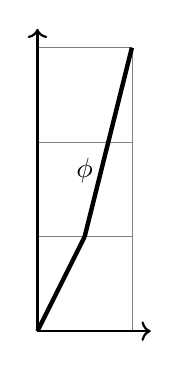
\begin{tikzpicture}[scale=1.2]
\draw[step=1,gray,very thin] (0,0) grid (1,3);
\draw [thick,->] (0,0) -- (1.2,0);
\draw [thick,->] (0,0) -- (0,3.2);
\draw [domain=0:0.5, ultra thick] plot (\x, 2*\x);
\draw [domain=0.5:1, ultra thick] plot (\x, 4*\x-1);
\draw (0.5,1.7) node {$\phi$};
\end{tikzpicture}
\qquad
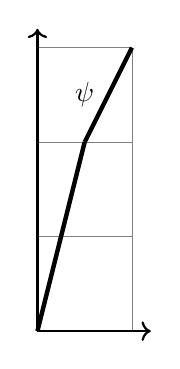
\begin{tikzpicture}[scale=1.2]
\draw[step=1,gray,very thin] (0,0) grid (1,3);
\draw [thick,->] (0,0) -- (1.2,0);
\draw [thick,->] (0,0) -- (0,3.2);
\draw [domain=0:0.5, ultra thick] plot (\x, 4*\x);
\draw [domain=0.5:1, ultra thick] plot (\x, 2*\x+1);
\draw (0.5,2.5) node {$\psi$};
\end{tikzpicture}
}
\begin{align*}
\phi\colon t& \mapsto \begin{cases}
4t & t\in [0,\frac12]\\
2t+1 & t\in [\frac12,1]
\end{cases}\\
\psi\colon t& \mapsto \begin{cases}
2t & t\in [0,\frac12]\\
4t-1 & t\in [\frac12,1]
\end{cases}
\end{align*}
with graphs as at right.

These two paths $I\to [0,3]$ are homotopic fixing endpoints by the homotopy $h_a(s,t) = 
s\phi(t) + (1-s) \phi(t)$. If we then precompose 
$\langle\gamma,\eta,\lambda\rangle\colon [0,3]\to X$ with $h_a\colon I\times I \to [0,3]$, 
we get a homotopy between $( \gamma \# \eta ) \# \lambda$ and $\gamma \# ( \eta 
\# \lambda)$. Path concatenation in $X$ is then \emph{homotopy associative}. But what 
about inverses or an identity element? We will play the same trick, by considering a 
`universal' case.

Given a path $\gamma\colon I \to X$, we have the reverse path $-\gamma$,
\marginnote{recall $-\gamma(t) := \gamma(1-t)$\\%} 
%\marginnote{%
\noindent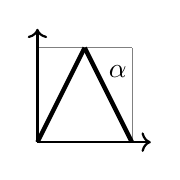
\begin{tikzpicture}[scale=1.2]
\draw[step=1,gray,very thin] (0,0) grid (1,1);
\draw [thick,->] (0,0) -- (1.2,0);
\draw [thick,->] (0,0) -- (0,1.2);
\draw [domain=0:0.5, ultra thick] plot (\x, 2*\x);
\draw [domain=0.5:1, ultra thick] plot (\x, 2-2*\x);
\draw (0.85,0.75) node {$\alpha$};
\end{tikzpicture}
\qquad
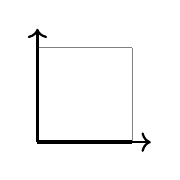
\begin{tikzpicture}[scale=1.2]
\draw[step=1,gray,very thin] (0,0) grid (1,1);
\draw [thick,->] (0,0) -- (1.2,0);
\draw [thick,->] (0,0) -- (0,1.2);
\draw [domain=0:1, ultra thick] plot (\x, 0);
% \draw [domain=0.5:1, ultra thick] plot (\x, 2-2*\x);
\end{tikzpicture}

\medskip

\noindent
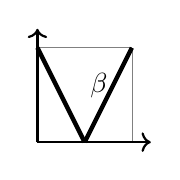
\begin{tikzpicture}[scale=1.2]
\draw[step=1,gray,very thin] (0,0) grid (1,1);
\draw [thick,->] (0,0) -- (1.2,0);
\draw [thick,->] (0,0) -- (0,1.2);
\draw [domain=0:0.5, ultra thick] plot (\x, 1-2*\x);
\draw [domain=0.5:1, ultra thick] plot (\x, 2*\x-1);
\draw (0.65,0.6) node {$\beta$};
\end{tikzpicture}
\qquad
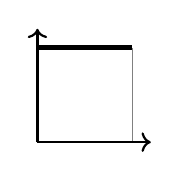
\begin{tikzpicture}[scale=1.2]
\draw[step=1,gray,very thin] (0,0) grid (1,1);
\draw [thick,->] (0,0) -- (1.2,0);
\draw [thick,->] (0,0) -- (0,1.2);
\draw [domain=0:1, ultra thick] plot (\x, 1);
% \draw [domain=0.5:1, ultra thick] plot (\x, 2-2*\x);
% \draw (0.5,2.5) node {$\psi$};
\end{tikzpicture}

\medskip

\noindent
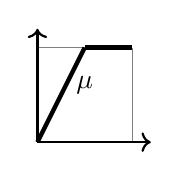
\begin{tikzpicture}[scale=1.2]
\draw[step=1,gray,very thin] (0,0) grid (1,1);
\draw [thick,->] (0,0) -- (1.2,0);
\draw [thick,->] (0,0) -- (0,1.2);
\draw [domain=0:0.5, ultra thick] plot (\x, 2*\x);
\draw [domain=0.5:1, ultra thick] plot (\x, 1);
\draw (0.5,0.6) node {$\mu$};
\end{tikzpicture}
\qquad
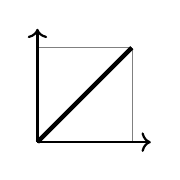
\begin{tikzpicture}[scale=1.2]
\draw[step=1,gray,very thin] (0,0) grid (1,1);
\draw [thick,->] (0,0) -- (1.2,0);
\draw [thick,->] (0,0) -- (0,1.2);
\draw [domain=0:1, ultra thick] plot (\x, \x);
% \draw [domain=0.5:1, ultra thick] plot (\x, 2-2*\x);
% \draw (0.5,2.5) node {$\psi$};
\end{tikzpicture}

\medskip

\noindent
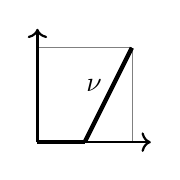
\begin{tikzpicture}[scale=1.2]
\draw[step=1,gray,very thin] (0,0) grid (1,1);
\draw [thick,->] (0,0) -- (1.2,0);
\draw [thick,->] (0,0) -- (0,1.2);
\draw [domain=0:0.5, ultra thick] plot (\x, 0);
\draw [domain=0.5:1, ultra thick] plot (\x, 2*\x-1);
\draw (0.6,0.6) node {$\nu$};
\end{tikzpicture}
\qquad
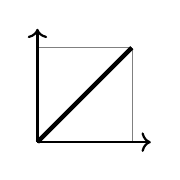
\begin{tikzpicture}[scale=1.2]
\draw[step=1,gray,very thin] (0,0) grid (1,1);
\draw [thick,->] (0,0) -- (1.2,0);
\draw [thick,->] (0,0) -- (0,1.2);
\draw [domain=0:1, ultra thick] plot (\x, \x);
% \draw [domain=0.5:1, ultra thick] plot (\x, 2-2*\x);
% \draw (0.5,2.5) node {$\psi$};
\end{tikzpicture}}
%
and the composite $\gamma \# (-\gamma)\colon I \to X$ can be factored as 
$I\xrightarrow{\alpha} I \xrightarrow{\gamma} X$ for a certain path $I\xrightarrow{\alpha} 
I$. If we instead concatenate in the other direction, namely $(-\gamma)\# \gamma\colon 
I\to X$, then this factors as $I\xrightarrow{\beta} I\xrightarrow{\gamma}X$. Again 
$\beta$ is a certain path in $I$. The graphs of both $\alpha$ and $\beta$ are shown at 
right, and both of them are homotopic, fixing endpoints, to the constant functions at 
$0$ and $1$ respectively, by taking an affine combination as in the definition of $h_a$ 
above. Then by composing the homotopies here with $\gamma$, we get homotopies between 
the path $\gamma\#(-\gamma)$ and the constant path at $\gamma(0)$, and also between 
$(-\gamma)\#\gamma$ and the constant path at $\gamma(1)$. So we have \emph{homotopy 
inverses}.

If we want to think about a homotopy identity element, then we should use the constant 
path $c_x\colon I\to X$ at a point $x\in X$, with $c_x(t)= x$, $\forall t\in I$. We can 
factor the composite $\gamma\# c_{\gamma(1)}$ as $I\xrightarrow{\mu} I 
\xrightarrow{\gamma} X$ for $\mu$ as shown at right, and factor $c_{\gamma(0)}\#\gamma$ 
as $I\xrightarrow{\nu} I \xrightarrow{\gamma} X$. As above, $\mu$ and $\nu$ are 
homotopic, fixing endpoints, to the identity map $I\to I$.

If we turn the five homotopies $I\times I \to X$ described above into paths $I\to X^I$, then if we start from elements of $\Omega_x X$, these homotopies correspond to paths in $\Omega_x X$.
Thus $\Omega_x X$, which has a concatenation binary operator $\#\colon \Omega_xX \times \Omega_xX\to \Omega_xX$, acts like a group, except the group axioms only hold up to the existence of paths\marginnote{More is true, though we won't prove it: there are homotopies assembled out of these paths for all possible cases, for instance $I \times \Omega_x X \times \Omega_x X \times \Omega_x X \to \Omega_x X$} 
\begin{align*}
( \gamma \# \eta ) \# \lambda & \rightsquigarrow \gamma \# ( \eta \# \lambda)\\
\gamma\# (-\gamma) &\rightsquigarrow c_{\gamma(0)}\\
(-\gamma)\# \gamma &\rightsquigarrow c_{\gamma(1)}\\
\gamma\# c_{\gamma(1)}&\rightsquigarrow \gamma \\
c_{\gamma(0)}\#\gamma &\rightsquigarrow \gamma
\end{align*}
in $\Omega_x X$. As a result we have proved most of

\begin{prop}
Let $(X,x)$ be a pointed space, with $X$ slsc.\marginnote{If we fall back on the default, namely just slpc, then we can use $[\pt,\Omega_x X]$ instead} The set $\pi_0(\Omega_x X)$ carries the 
structure of a group, its product arising from concatenation of loops and identity element 
represented by the constant path at $x$.
\end{prop}

\begin{proof}
To exhibit the multiplication, consider the functor $\pi_0$ applied\marginnote{This requires knowing that $\#$ is continuous! See Assignment 2.} to $\#\colon \Omega_x X 
\times \Omega_x X \to \Omega_x X$, giving $\pi_0(\Omega_x X \times \Omega_x X) \xrightarrow{\#} 
\pi_0(\Omega_x X)$. But since $\pi_0(M\times N) \xrightarrow{\simeq} 
\pi_0(M)\times\pi_0(N)$, for all slpc spaces $M$ and $N$, we get a composite 
$\pi_0(\Omega_x X) \times \pi_0(\Omega_x X) \simeq \pi_0(\Omega_x X \times \Omega_x X) 
\to \pi_0(\Omega_x X)$. This is associative and unital, and inverses exist, by the 
existence of the paths above.
\end{proof}

\begin{definition}
For\marginnote{Recall we also proved $[\pt,-]$ descends to a functor $\Ho \to \Set$ in Assignment 1}
 $(X,x)$ a pointed space its \emph{fundamental group at $x$} is 
$\pi_1(X,x) := [\pt,\Omega_xX]$, which for $X$ a slsc space coincides with $\pi_0(\Omega_xX)$.
\end{definition}

From\marginnote{As a point of clarification, everything here works for arbitrary slpc spaces with small adjustments, but for slsc spaces the approach is slightly cleaner, as components and path components coincide for the function spaces} the previous reasoning, we have constructed from a covering space $Z\to X$ and 
chosen basepoint $x\in X$ a permutation representation $\pi_1(X,x) \to \Aut(Z_x)$. If 
$Z$ is path connected, and we choose $z\in Z_x$, we get a surjective map $\pi_1(X,x) \to 
Z_x$, given by $\gamma\mapsto \gamma_*(z)$. This implies we have an upper bound on the 
cardinality of fibres of any path connected covering space, and conversely, given a 
connected covering space, the fibres give a lower bound on the number of distinct 
homotopy classes of loops in $X$.

\begin{example}
The projection map $S^2 \to \mathbb{RP}^2$ is a covering space and $S^2$ is connected, 
so there exist at least two non-homotopic loops in $\mathbb{RP}^2$ at any given 
basepoint. One of these is the constant loop, so there exists a loop in $\mathbb{RP}^2$ 
not homotopic to it.
\end{example}

\begin{example}\label{eg:piS^1_infinite}
We have the covering space $\exp(2\pi i-)\colon \RR\to S^1$ with fibre
$\ZZ$ over $1\in S^1$, which implies $\pi_1(S^1,1)$ is an infinite group.
\end{example}

\begin{prop}
The loop space construction is a functor $\Omega\colon \Top_*\to \Top_*$.
\end{prop}


\begin{corollary}
The fundamental group\marginnote{Exercise: This functor is naturally isomorphic to $[(S^1,1),(X,x)]_*$} gives a functor 
\[
	\pi_1 := [\pt,-] \circ \Omega\colon \Top_*\to \Grp.
\]
which for slsc spaces is naturally isomorphic to $\pi_0\circ \Omega$.
\end{corollary}


However,\lecturenum{8} as we have seen, we don't just get an action of $\pi_1(X,x)$ on the fibre $Z_x$ 
of a covering space. We also get what looks like an action of paths between different 
points on fibres, but now points in one fibre are taken to points of another fibre. In 
fact, if $X$ is not equipped with a basepoint to start with, or there are several 
natural options and no one of those is canonical, then we can create an even richer 
invariant, namely a \emph{groupoid}.

\begin{definition}
A \emph{groupoid} is a category where every morphism has an inverse.
\end{definition}

So that we have an idea of what kinds of groupoids arise, let us consider some examples. 
We will be considering only \emph{small} groupoids: those locally small groupoids 
$\Gamma$ where there is a set $\Gamma_0$ of objects. We can then take the disjoint union 
of all the hom-sets to get the set $\Gamma_1= \bigsqcup_{x,y\in \Gamma_0} \Gamma(x,y)$ of morphisms, and specify the source and 
target functions $s,t\colon \Gamma_1\rightrightarrows \Gamma_0$. Groupoids and functors 
form a category $\Gpd$.

\begin{example}
\begin{enumerate}
\item Every set $S$ gives a groupoid $\disc(S)$, by taking the set of objects to be $S$, and to only have identity
morphisms. This gives a full subcategory inclusion $\disc\colon \Set \into \Gpd$, and such groupoids are called \emph{discrete}.
\item Every set $C$ also gives another groupoid $\codisc(C)$ with set of objects $C$, but with exactly 
one morphism from any object to any other object. The set of morphisms is $C\times C$, and every 
object $c\in C$ has the trivial group of automorphisms. Such groupids are called \emph{codiscrete}.
\item Let $G$ act on the set $Y$ on the right. Then there is a groupoid $Y/\!/G$ with object set $Y$, and set of 
morphisms $Y\times G$. The source and target are given by $s(y,g)=y$, $t(y,g)=yg$, and composition is $(y,g)(yg,h) = (y,gh)$.
\begin{enumerate}
\item If $G=1$, then this recovers the first example.
\item If $Y=\pt$, then the information in the groupoid is essentially just that of the group $G$. Groupoids of this form will be denoted $\BB G$, and $\BB\colon \Grp \into \Gpd$ is the inclusion of a full subcategory.
\end{enumerate}
\end{enumerate}
\end{example}

A slogan people sometimes use is that a groupoid is like a group with `many identities', 
but you can also usefully think of them as being a generalisation of a group action, 
where you have different groups acting on different parts of the set. Here is a useful 
lemma about the structure of groupoids.

\begin{lemma}
For any groupoid $\Gamma$, and given $x,y\in \Gamma_0$,\marginnote{using algebraic order of composition}
\begin{align*}
	\Ad_a\colon \Gamma(x,x) & \xrightarrow{\simeq} \Gamma(y,y)\\
			g & \mapsto a^{-1}ga
\end{align*}
is an isomorphism for any $a\in \Gamma(y,x)$\marginnote{$(\Ad_a)^{-1} = \Ad_{a^{-1}}$\\\bigskip\noindent transitive: $(ba^{-1},a) \mapsto b$;\\ 
\noindent free: $ga=a$ implies $g = gaa^{-1} = aa^{-1} =\id_x$} and 
the function
\begin{align*}
	\Gamma(x,x)\times \Gamma(x,y) & \to \Gamma(x,y)\\
		(g,a) & \mapsto ga
\end{align*}
defines a free and transitive action of the group $\Gamma(x,x)$.
\end{lemma}

As a reminder: a free group action $G\times S\to S$ is one where $g\cdot p = p$ implies 
$g$ is the identity element, and a transitive action one where given any two elements 
$p,q\in S$, there is some group element $g\in G$ such that $g\cdot p = q$.

\begin{definition}
Given an slsc space $X$ and a specified subset $A\subseteq X$, the \emph{fundamental groupoid 
based at $A$}
is the groupoid $\Pi_1(X,A)$ with set of objects $A$, and the set of morphisms from $x$ to $y$ is $\Pi_1(X,A)(x,y) := \pi_0(P_x^yX)$. 
The\marginnote{the definition makes sense for more general slpc spaces, using $[\pt,-]$ in place of $\pi_0$, but we are only consider slsc spaces here} composition map is induced from concatenation of paths:
\[
	\pi_0(P_x^yX) \times \pi_0(P_y^zX) \simeq \pi_0(P_x^y X\times P_y^zX) \to \pi_0(P_x^zX)
\]
and 
constant paths are the identity morphisms.
\end{definition}


As with other invariants, the fundamental groupoid is a functor. Define the category 
$\Top^{(2)}$ to be the category with objects pairs $(X,A)$ where $X$ is a topological 
space and $A\subseteq X$ is a subspace, and a morphism $(X,A) \to (Y,B)$ is a continuous 
function $f\colon X\to Y$ such that $f(A) \subseteq B$. We have a full subcategory inclusion 
$\Top_*\into \Top^{(2)}$.

\begin{prop}
The fundamental groupoid gives a functor $\Pi_1\colon \Top^{(2)}\to \Gpd$ such that
\[
	\xymatrix{
		\Top_* \ar[r]^{\pi_1} \ar[d] & \Grp \ar[d]^{\BB}\\
		\Top^{(2)} \ar[r]_{\Pi_1} & \Gpd
	}
\]
and moreover:\marginnote{The product/disjoint union of groupoids is 
what you think it is: take the products/disjoint unions of the objects and the morphisms, respectively} 
\begin{align*}
	\Pi(X\times Y,A\times B) & \xrightarrow{\simeq} \Pi_1(X,A) \times \Pi_1(Y,B)\\
	\Pi_1(X,A) \sqcup \Pi_1(Y,B) & \xrightarrow{\simeq} \Pi(X\sqcup Y,A\sqcup B)
\end{align*}
\end{prop}

We can include \emph{unbased} spaces $X$ into pairs, by taking $(X,X)$, giving another 
fully faithful functor, $\Top \to \Top^{(2)}$. In this case, if the space $X$ has 
\emph{no} preferred basepoints whatsoever, we can still define the fundamental groupoid 
of $X$ itself as $\Pi_1(X,X)$, which is a functor $\Top \to \Gpd$.


We haven't yet seen how to calculate the fundamental group(oid) in 
examples, so we will turn to that now. We need a name for spaces $X$ that have 
$\Pi_1(X)$ trivial, in the sense of being codiscrete.

\begin{definition}
A space $X$ that satisfies $\Pi_1(X) = \codisc(X)$\marginnote{such spaces 
also have $\Pi_1(X,A) = \codisc(A)$ for all $A\subseteq X$} is called 
\emph{simply-connected}.
\end{definition}

If we unpack this definition, it tells us that a) given any two points $x,y\in X$, there is a (homotopy class of some) path from $x$ to $y$, so that $X$ is path-connected, and b) all paths between any two given points are endpoint-fixed homotopic, hence a unique morphism in the fundamental groupoid. 
As a result, $\pi_1(X,x) = \Pi_1(X)(x,x)$ is the trivial group.

\begin{example}
Convex subspaces $C\subseteq \RR^n$ are simply-connected, because any two points $v,w\in C$ 
can be joined by a path in $C$, and given two paths $\gamma,\eta\colon v\rightsquigarrow w$
the map $(s,t)\mapsto s\gamma(t)+(1-s)\eta(t)$ is a homotopy between them.
\end{example}

In particular, the interval $I$ is simply-connected. The fundamental groupoid $\Pi_1(I,\{0,1\})$
is important enough to have its own name: $\mathbf{2}$, sometimes denoted 
$(0\xrightarrow{\sim} 1)$, as it has two objects $0,1$ and a unique isomorphism between them.

\begin{ex}
Define a \emph{star-shaped region}\marginnote{For $\mathcal{H} \subset \CC$ the
(open) upper half-plane, the set $\mathcal{H}\cup\mathbb{Q}$ is star-shaped, but not convex} 
in a (real or complex) vector space $V$ to be a set 
$K\subseteq V$ such that there is a point $v_0\in K$ such that for every $v\in K$ and $t\in I$,
$tv_0+(1-t)v\in K$. Prove that star-shaped regions are simply-connected.
\end{ex}

Simply-connected spaces are special for the following reason.

\begin{prop}
If $X$ is a simply-connected space, then every path connected covering space 
$Z\xrightarrow{\pi} X$ is trivial, in the sense that $\pi$ is a homeomorphism.
\end{prop}

\begin{proof}
Recall that $\pi_1(X,x) \to Z_x$ is surjective for any $x\in X$, so $X$ simply-connected implies
$Z_x = \pt$ for all $x$. Thus $\pi$ is a bijection. The local triviality condition implies 
that every $x\in X$ has an open set $U\ni x$ such that $\pi^{-1}(U) \to U$ is a homeomorphism. 
Letting $U_\alpha$ range over such an cover of $X$, we can glue the inverses of these local 
homeomorphisms into an inverse for $\pi$.
\end{proof}



\begin{example}
If $X$ is contractible then it is simply-connected. Let $H\colon I\times X \to X$ be a 
contraction to $x_0\in X$. Consider the induced map $h= \Pi_1(H)\colon \Pi_1(I\times X, 
\{0,1\}\times X) \to \Pi_1(X,X) = \Pi_1(X)$. The domain simplifies to be 
$\Pi_1(I,\{0,1\})\times \Pi_1(X) = \mathbf{2}\times \Pi_1(X)$. Consider the induced maps 
$\{i\}\times \Pi_1(X)\to \mathbf{2}\times \Pi_1(X) \to \Pi_1(X)$ for $i=0,1$. Since 
$H\big|_{\{0\}\times X}=\id_X$, so $h_{\{0\}\times \Pi_1(X)}=\id_{\Pi_1(X)}$; and as 
$H\big|_{\{1\}\times X}$ is constant at $x_0$, so $h(0,x) = x_0$ for all $x\in X$, and 
$h\big|_{\{1\}\times \Pi_1(X)}$ sends every path to the constant path at $x_0$. We 
already know that $X$ is path connected, so that for any $x,y\in X$ there is some path 
between them. Given a path $\gamma\colon x\rightsquigarrow y$ consider the commutative square
\[
	\xymatrix{
	(0,x) \ar[r]^{(\id_0,[\gamma])} \ar[d] & (0,y) \\
	(1,x) \ar[r]_{(\id_1,[\gamma])} & (1,y) \ar[u]
	}
\]
in $\mathbf{2}\times \Pi_1(X)$ (recall all morphisms are invertible). Under $h$ this is sent to
\[
	\xymatrix{
	x\ar[r]^{[\gamma]} \ar[d] & y \\
	x_0 \ar[r]_{\id} & x_0 \ar[u]
	}
\]
The vertical arrows are independent of $[\gamma]$, so that every path $\gamma$ in $X$ is 
homotopic to the composite the long way around the square, hence to every other path.
\end{example}

So\lecturenum{9} in some sense, we are interested in spaces that are path connected, though this is 
useful when building spaces out of disjoint components. Here is another way we can get 
information about the fundamental groupoid of a space from the fundamental groupoid of 
other spaces.

\begin{theorem}\label{thm:cov_space_gives_faithful_functor}
Let $Z\xrightarrow{\pi} X$ be a covering space.\marginnote{thus the funtor $\Pi_1(\pi)$ is \emph{faithful}} 
Then $\Pi_1(Z)(z_1,z_2) \to \Pi_1(X)(\pi(z_1),\pi(z_2))$ is injective for all $z_1,z_2\in Z$.
\end{theorem}

We will prove this theorem in a little bit, but let us give an important result that follows.

\begin{corollary}
Given a covering space $(Z,z)\xrightarrow{\pi}(X,x)$, the induced homomorphism between fundamental groups identifies $\pi_1(Z,z)$ with a subgroup of 
$\pi_1(X,x)$.
\end{corollary}

This allows us, given a covering space whose fundamental groupoid we know, to place a 
lower bound on the size of the fundamental group of the base space. Alternatively, it 
places an upper bound on the size of the fundamental group of the covering space, so if 
$\pi_1(X,x)$ is finite, then so is $\pi_1(Z,z)$.

\begin{prop}\label{prop:cov_space_of_IxX}
Let $Z\to I\times X$ be a covering space. Then $Z\xrightarrow{\simeq} I\times Z_0$ over 
$I\times X$, where $Z_0 := Z_{\{0\}\times X}$.
\end{prop}

\begin{proof}
The function $Z\to I\times Z_0$ is given by $(\pr_1\circ \pi,\tau)$, for some 
$\tau\colon Z\to Z_0$, which we need to construct.
The idea is similar to the situation where we constructed the trivialisation of a 
covering space of $I$, which is the special case of $X=\pt$. 
Given $x\in X$, we get a trivisalisable covering space $Z_{I\times \{x\}}\to I\times \{x\}\simeq I$, and so 
a function $\tau_x\colon Z_{I\times \{x\}} \to I\times Z_{(0,x)} \xrightarrow{\pr_2}Z_{(0,x)}$. 
Hence we have a (potentially discontinuous) function $Z \to Z_0$ using the various $\tau_x$. 
We will write down a global version of this function using ingredients we already know to be 
continuous.

Given $(t,x)\in I\times X$, there is a path $(0,x) \rightsquigarrow (t,x)$ given by
$\eta_{(t,x)}(s) = (ts,x)$, which we want to vary continuously with $(t,x)$. We know that 
$I\times I \times X\to I\times X$, $(s,t,x) \mapsto (ts,x)$ is continuous, so that by the 
\begin{align*}
	I\times X & \to (I\times X)^I\\
	(t,x) & \mapsto \eta_{(t,x)}
\end{align*}
is continuous. We can now define the composite
\begin{align*}
	\tau\colon Z & \xrightarrow{\simeq} (I\times X)\times_{I\times X} Z \to (I\times X)^I \times_{I\times X} Z 
	\xrightarrow{\Lift} Z^I\xrightarrow{\ev_1} Z\\
	z&\mapsto (\pi(z),z)\qquad \mapsto\quad (-\eta_{\pi(z)},z)
\end{align*}
This map factors through $Z_0$, as if $(t,z) :=\pi(z)$, then $-\eta_z$ is a path in $I\times X$ 
from $(t,x)$ to $(0,x)$ and so the evaluation of the lift of $-\eta_z$ at $1$ sits over $(0,x)$.
Since all the maps here are continuous, $\tau$ is continuous.

We need to supply a continuous inverse to $(\pr_1\circ \pi,\tau)$, which is built the 
same way, except now using $\eta_z$ itself to lift, rather than $-\eta_z$:
\[
	\sigma\colon I\times Z_0 \to (I\times X)^I\times_{I\times X} Z \xrightarrow{\Lift}
	Z^I \xrightarrow{\ev_1} Z.
\]
This is manifestly continuous, and one can check that this map is the required inverse by
considering the composite at each point separately, where it reduces to considering $Z$ 
restricted to $I\times \{x\}$.
\end{proof}

\begin{corollary}\label{prop:pullback_by_homotopic_maps_iso}
If $f,g\colon X\to Y$ are homotopic, say by $H\colon I\times X \to Y$, and $Z\to Y$ is a 
covering space, then $f^*Z\simeq g^*Z$ over $X$.
\end{corollary}

\begin{proof}
If we form $H^*Z\to I\times X$, then we have by Proposition~\ref{prop:cov_space_of_IxX}
that $H^*Z \simeq I\times f^*Z$. But $g^*Z \to X$ is (isomorphic to)  
$(H^*Z)_{\{1\}\times X}$, hence is isomorphic to $(I\times f^*Z)_{\{1\}\times X}$, but this
is isomorphic to $f^*Z$.
\end{proof}

This gives us a criterion whereby we know that no interesting covering spaces exist

\begin{corollary}
If $X$ is contractible, then every covering space $Z\to X$ is isomorphic to $X\times Z_x$ 
for any $x\in X$.
\end{corollary}

\begin{proof}
Let $H\colon I\times X \to X$ be a contraction to $x\in X$\marginnote{Exercise: such a contraction exists for all $x\in X$}. Then for $c_x\colon X\to X$ the 
constant map at $x$, $c_x^*Z = X\times Z_x$. But $H$ is a homotopy between $\id_X$ and $c_x$,
and $\id^*Z = Z$, so by Corollary~\ref{prop:pullback_by_homotopic_maps_iso} we have the required
isomorphism.
\end{proof}

\begin{example}
Any locally convex topological vector space has no interesting covering spaces, likewise any convex or even star-shaped region therein.
The unit sphere in a separable, infinite-dimensional Hilbert space has no interesting covering
spaces. The infinite-dimensional Stiefel manifolds likewise.
\end{example}


\begin{corollary}
Let\marginnote{%
$\xymatrix{
\{0\}\times X \ar[d] \ar[r]^-{\widetilde{f}} & Z \ar[d]^\pi\\
I\times X \ar@{-->}[ur]^{\widetilde{H}} \ar[r]_-{H} &Y
}$}
$Z\xrightarrow{\pi} Y$ be a covering space, $f,g\colon X\to Y$ a pair of maps and 
$H\colon I\times X\to Y$ a homotopy from $f$ to $g$. If $\widetilde{f}\colon \{0\}\times 
X\to Z$ is a lift of $f$, in the sense that the diagram at right commutes, then there is 
a unique homotopy $\widetilde{H}\colon I\times X \to Z$ lifting $H$ from $\widetilde{f}$ 
to a lift of $g$.
\end{corollary}

\begin{proof}
Since $I\times f^*Z \xrightarrow{\simeq} H^*Z$, and we have a section $X\to f^*Z$, then 
we get a section $I\times X \to I\times f^*Z$. Composing with the isomorphism we get a 
map $I\times X \to I\times f^*Z \to H^* Z \to Z$, and this both restricts to 
$\widetilde{f}$ on $\{0\}\times X$ and covers $H$. To show uniqueness, notice that 
$H(-,x)$ gives a path in $Y$ for each fixed $x\in X$. Any lift $\widetilde{H}'$ of $H$ 
likewise gives a path $\widetilde{H}'(-,x)$ for fixed $x$. Since lifts of paths are unique, the 
$\widetilde{H}'(-,x)$ must agree with $\widetilde{H}(-,x)$ for all $x$, hence 
$\widetilde{H}'=\widetilde{H}$.
\end{proof}

We can now give the promised proof of Theorem~\ref{thm:cov_space_gives_faithful_functor}.

\begin{proof}
(of Theorem~\ref{thm:cov_space_gives_faithful_functor}) Given paths $\gamma,\eta\colon z_1 \rightsquigarrow z_2$ in $Z$, and an endpoint-fixing homotopy 
$H\colon I\times I \to X$ between $\pi\circ \gamma$ and $\pi\circ\eta$, we can lift $H$ to give
a homotopy from $\gamma$ to a lift of $\pi\circ \eta$. Since $H$ fixes endpoints, the lifts of
the constant paths $H\big|_{I\times\{i\}}$, for $i=0,1$ are path in the fibre, discrete spaces.
Hence these paths are constant, and $\widetilde{H}$ is a homotopy fixing endpoints.
Since $\eta$ is a lift of $\pi\circ \eta$, unique path lifting gives that $\widetilde{H}$ is 
in fact a homotopy (fixing endpoints) from $\gamma$ to $\eta$. Thus $\gamma$ and $\eta$ give
the same element in $\Pi_1(Z)(z_1,z_2)$, and the induced map in injective as required. 
\end{proof}

Until now, a lot of our resuls only give bounds on or estimates between the fibres of a covering
space and the fundamental group of the base space. However, we can actually get an exact result, given a certain kind of covering space

\begin{theorem}
If $\pi\colon (Z,z) \to (X,x)$ is a covering space with $Z$ path connected, then  
\[
Z_x \simeq \pi_1(X,x)/\pi_1(Z,z),
\]
as sets with $\pi_1(X,x)$-action.
\end{theorem}

\lecturenum{10}

\begin{proof}

There\marginnote{For a group $G$, sets with a $G$-action will be called 
\emph{$G$-sets}.}  is in fact a canonical isomorphism, induced in the following way. For 
group $G$ and any transitive $G$-set $S$, and a point $p\in S$, then the map $G \to S$, 
$g\mapsto g\cdot s$ induces a well-defined bijection $G/\mathrm{Stab}(s) \to S$, where 
$\mathrm{Stab}(s) < G$ is the subgroup of elements $g$ such that $g\cdot s = s$ (the 
\emph{stabiliser subgroup}). Notice that for \emph{any} subgroup $H< G$, $G/H$ inherits 
a $G$-action from the multiplication in $G$. And the bijection $G/\mathrm{Stab}(s) \to S$ is 
compatible with the $G$-actions\marginnote{that is, \emph{equivariant}}.

We apply this to the transitive $\pi_1(X,x)$-set $Z_x$, where we know the action is 
transitive as $Z$ is path-connected. This gives an isomorphism 
$\pi_1(X,x)/\mathrm{Stab}(z) \xrightarrow{\simeq} Z_x$, and it remains to identify 
$\mathrm{Stab}(z) < \pi_1(X,x)$. But note that if for some $[\gamma] \in \pi_1(X,x)$, 
$\gamma_*(z)=z$, this means that the lift $\widetilde{\gamma_z}$ beginning at $z$ also 
ends at $z$, so is a loop in $Z$. Thus $\mathrm{Stab}(z)$ consists of the homotopy 
classes of loops in $X$ that come from loops in $Z$, that is, $\mathrm{Stab}(z) = 
\pi_1(Z,z)$.
\end{proof}




\begin{corollary}\label{cor:fibre_of_univ_cov_space}
If $\pi\colon (Z,z) \to (X,x)$ is a covering space with $Z$ simply-connected, then the map
\[
\pi_1(X,x) \to Z_x
\]
is an isomorphism of $\pi_1(X,x)$-sets.
\end{corollary}


\begin{proof}
Since $Z$ is simply-connected, $\pi_1(Z,z) = 1$, and so $\pi_1(X,x) \to Z_x$ is an isomorphism
of sets with $\pi_1(X,x)$-action.
\end{proof}

\begin{example}
We now can say that $\pi_1(S^1,1)$ is not just infinite (see Example~\ref{eg:piS^1_infinite})
 but countable, since it is in bijection with the fibre $\ZZ$ of the simply-connected covering space $\RR \to S^1$.
\end{example}

But even better, we have not just a bijection, but Corollary 
\ref{cor:fibre_of_univ_cov_space} gives a \emph{faithful permutation representation}: 
given $[\gamma],[\eta]\in \pi_1(X,x)$, there is some $z\in Z_x$ such that 
$\gamma_*(z)\neq \eta_*(z)$, which is equivalent to $\pi_1(X,x) \to \Aut(Z_x)$ being 
injective. Thus we have represented the fundamental group of $(X,x)$ as a permutation 
group, where we can do more concrete computations.

\begin{corollary}
For $(Z,z)\to (X,x)$ a simply-connected covering space, $\pi_1(X,x)$ acts freely on $Z_x$.
\end{corollary}

And now we can give the first example of an actually calculated, non-trivial fundamental group.

\begin{theorem}
$\pi_1(S^1,1) \simeq \ZZ$.
\end{theorem}

\begin{proof}
We have the simply-connected covering space $\RR \to S^1 = \RR/\ZZ$, with fibre over 
$1\in S^1$ being the integers. The inclusion $[0,1]\to \RR$ is a lift of the loop $\gamma$ 
going once around the circle, and all lifts are translates of this, so that the action of 
$\gamma$ on the fibre $\ZZ$ is translation by $1$. The loop $\gamma$ generates a subgroup
whose action on $\ZZ$ is transitive, hence $\gamma$ generates all of $\pi_1(S^1,1)$,
which must then be infinite cyclic, hence $\ZZ$.
\end{proof}

As a result, for any subset $A\subset S^1$, the fundamental groupoid $\Pi_1(S^1,A)$ has as 
objects the set $A$, for every $x\in A$, $\pi_1(S^1,x) \simeq \ZZ$, and for any two points
$x,y\in S^1$, the hom-set $\Pi_1(S^1,A)(x,y)$ is isomorphic as a set to $\ZZ$.


But how do we calculate $\pi_1$ in general? Or better, $\Pi_1$? Recall that $\Pi_1(X,A) = \Pi_1(X_1,A\cap X_1) \sqcup
\Pi_1(X_2,A\cap X_2)$.
For instance, if $X_1$ and $X_2$ are the only path components of $X$, and 
$\exists x\in A\cap X_i$ for $i=1,2$, then every point in $X$ is connected by a path to a point
in $A$. This means the fundamental goups of the two path components are captured.

\begin{example}
Consider $\Pi_1(S^1\sqcup S^1,1\sqcup 1)$, which is a groupoid with two objects, both of which
have automorphism groups given by $\ZZ$.
\end{example}

So we are going to focus a bit on calculating the fundamental group(oid) for path 
connected spaces. The easiest way to make a new connected space from two other connected spaces $X,Y$, say\marginnote{recall that we are taking spaces to be semilocally path connected, so that components and path components coincide}, is to take a point in each, $x\in X$, $y\in Y$, and identify $x$ and $y$.

\begin{definition}
Given\marginnote{A key property of the join is that given a pointed space $(M,m)$ and a pair of pointed 
maps $f\colon (X,x) \to (M,m)$, $g\colon (Y,y) \to (M,m)$, there is a unique pointed map 
$\langle f,g\rangle\colon (X\vee Y,\ast) \to (M,m)$ such that $f = \mathrm{in}_L\circ 
\langle f,g\rangle$ and $g = \mathrm{in}_R\circ \langle f,g\rangle$.} two pointed spaces $(X,x)$ and $(Y,y)$, the \emph{join} $X\vee Y$ is the quotient 
space $(X\sqcup Y)/(x\sim y)$. It has a basepoint given by $*:=[x] = [y]$, and the 
inclusion maps of $(X,x)\xrightarrow{\mathrm{in}_L} (X\vee Y,*) \xleftarrow{\mathrm{in}_R} (Y,y)$ are pointed.
\end{definition}



Since we have pointed maps, we get from functoriality of $\pi_1$ two 
homomorphisms $\pi_1(X,x) \to \pi_1(X\vee Y,*) \leftarrow \pi_1(Y,y)$. 
If we already know what the fundamental groups of $X$ and $Y$ are, then we 
can try to leverage this knowledge to tell us something about the fundamental group
of the join. For instance, taking $X = Y = S^1$, we get homomorphisms 
\[
\ZZ \xrightarrow{\pi_1(\mathrm{in}_L)} \pi_1(S^\vee S^1,\ast) \xleftarrow{\pi_1(\mathrm{in}_R)} \ZZ
\]
Let\marginnote{%
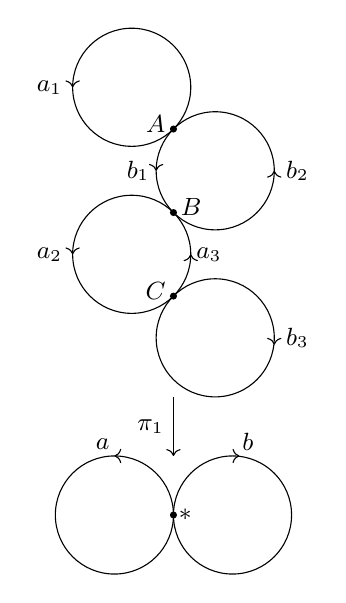
\begin{tikzpicture}[scale=1.5]
\draw[decoration={markings, 
                    % mark=at position 0 with {\arrow{>}};,
                    mark=at position 0.5 with {\arrow{>}}},
                    postaction={decorate}]
        ({-1/(2*sqrt(2))},{1.5+3/sqrt(2)}) circle (0.5);
\draw (-1.05,{1.5+3/sqrt(2)}) node {\small $a_1$};
\fill (0,{1.5+2.5/sqrt(2)}) circle (0.03);
\draw (-0.15,{1.9+2/sqrt(2)}) node {\small $A$};    

\draw[decoration={markings, 
                    mark=at position 0 with {\arrow{>}};,
                    mark=at position 0.5 with {\arrow{>}}},
                    postaction={decorate}]
        ({1/(2*sqrt(2))},{1.5+2/sqrt(2)}) circle (0.5);
\draw (-0.3,{1.5+2/sqrt(2)}) node {\small $b_1$};
\draw (1.05,{1.5+2/sqrt(2)}) node {\small $b_2$};
\fill (0,{1.5+1.5/sqrt(2)}) circle (0.03);
\draw (0.15,{1.9+1/sqrt(2)}) node {\small $B$};

\draw[decoration={markings, 
                    mark=at position 0 with {\arrow{>}};,
                    mark=at position 0.5 with {\arrow{>}}},
                    postaction={decorate}]
        ({-1/(2*sqrt(2))},{1.5+1/sqrt(2)}) circle (0.5);
\draw (0.3,{1.5+1/sqrt(2)}) node {\small $a_3$};
\draw (-1.05,{1.5+1/sqrt(2)}) node {\small $a_2$};
\fill (0,{1.5+0.5/sqrt(2)}) circle (0.03);
\draw (-0.15,{1.9}) node {\small $C$};        

\draw[decoration={markings, 
                    mark=at position 0 with {\arrow{<}}},
                    postaction={decorate}]
        ({1/(2*sqrt(2))},1.5) circle (0.5);
\draw (1.05,{1.5}) node {\small $b_3$};

\draw[->] (0,1) -- (0,0.5)  node[midway,left] {\small $\pi_1$} ;

\draw[decoration={markings, mark=at position 0.25 with {\arrow{>}}},postaction={decorate}]
        (-0.5,0) circle (0.5);
\draw (-0.6,0.6) node {\small $a$};
\draw[decoration={markings, mark=at position 0.25 with {\arrow{<}}},postaction={decorate}]
        (0.5,0) circle (0.5);
\draw (0.63,0.62) node {\small $b$};
\fill (0,0) circle (0.03);
\draw (0.1,0) node {\small $\ast$};


\end{tikzpicture}}
us define $a,b\in \pi_1(S^1\vee S^1,\ast)$ to be the classes $\pi_1(\mathrm{in}_L)(1)$ and
$\pi_1(\mathrm{in}_R)(1)$ respectively.

Define the covering space $Z_1 \xrightarrow{\pi_1} S^1\vee S^1$ as at right, where 
$A,B,C \mapsto \ast$, and $a_i\mapsto a$, $b_i\mapsto b$, $i=1,2,3$. Then we get a 
representation $\rho_1\colon \pi_1(S^1\vee S^1,\ast)\to \Aut\{A,B,C\} \simeq S_3$. 
Looking at how paths representing $a$ and $b$ lift, we get $\rho_1(a) = (BC)$ and 
$\rho_1(b) = (AB)$, cycles in $S_3$. Calculating $\rho_1(ab)$ we get $(ABC)$, and 
similarly for $\rho_1(ba)$, to get $(ACB)$, so that $rho_1(ab) \neq \rho_1(ba)$.
As a result, we must have had $ab \neq ba$ in $\pi_1(S^1\vee S^1,\ast)$, or in other words,
the fundamental group of $S^1\vee S^1$ is \textbf{non-abelian}.

By a judicious choice of covering spaces, we can also prove that the two homomorphism 
$\ZZ \to \pi_1(S^1\vee S^1,\ast)$ are injective, so that $a$ and $b$ generate infinite 
cyclic subgroups. We will\marginnote{We can present $\ZZ\ast\ZZ$ as $\langle a,b|\ 
\rangle$, which has as elements $a^{n_1}b^{m_1}\ldots a^{n_k}b^{m_k}$ for $k\geq 1$ and 
$n_i,m_i\in \ZZ$, with $a^0=e=b^0$} later prove that $\pi_1(S^1\vee S^1,\ast) \simeq 
\ZZ\ast \ZZ = F_2$, a free group on the generators $a,b$.


\lecturenum{11}

\begin{definition}
The \emph{free group on $n$-symbols}, $F_n$ is any group with presentation 
\[
	\langle x_1,\ldots,x_n\mid\ \rangle.
\]
That is, generators $x_1,\ldots,x_n$ and no relations.
\end{definition}

The symbols are of course arbitrary. Elements in $F_n$ are (finite) words in $x_i$ and $x_i^{-1}$, with the empty word $()$ being the identity element, and with concatenation of words being the multiplication in $F_n$.

\begin{definition}
Given groups $G$ and $H$, the \emph{free product} $G\ast H$ of $G$ and $H$ is a group equipped with homomorphisms $i\colon G\to G\ast H$, $j\colon H \to G\ast H$, satisfying the following property: given any group $K$ and homomorphisms $\phi\colon G \to K$, $\psi\colon H\to K$, there exists a unique homomorphism $\kappa\colon G\ast H \to K$ such that $\phi = i\circ \kappa$ and $\psi=j\circ \kappa$.
\end{definition}


We can write things like this:
\[
	\xymatrix{
		& H \ar[d]^j \ar@/^1pc/[rdd]^\psi &\\
		G \ar[r]^i \ar@/_1pc/[drr]_\phi & G\ast H \ar@{-->}[dr]^{\exists!}_\kappa &\\
		&& K
	}
\]
The existence of the unique $\kappa$ given the data of $\phi$ and $\psi$ is the \emph{universal property} of the free product.

If\marginnote{here each $R_i$ and $Q_j$ are \emph{relations}: equations involving the given generators of $G$ and $H$ respectively} $G = \langle g_1,\ldots,g_m\mid R_1,\ldots, R_n\rangle$  and $H = \langle h_1,\ldots, h_k \mid Q_1,\ldots, Q_l\rangle$ are presentations of $H$ and $G$, then
\[
	G\ast H = \langle g_1,\ldots,g_m,h_1,\ldots,h_k \mid R_1,\ldots, R_n,Q_1,\ldots,Q_l\rangle
\]


The free product of groups is an example of a more general construction, the \emph{free product with amalgamation}, but this is again an example of a general construction that makes sense in an arbitrary category.

\begin{definition}
Let $\cC$ be an arbitrary category. A \emph{pushout square} is a commutative square
\[
	\xymatrix{
		W\ar[r]^b \ar[d]_a & Y \ar[d]^d \\
		X \ar[r]_c & P
	}
\]
in $\cC$ such that for any pair of morphisms $X\xrightarrow{f} Z \xleftarrow{g} Y$ such that 
$f\circ a = g\circ b$,\marginnote{this unique existence is the \emph{universal property} of the pushout}
\[
	\exists!\ P\xrightarrow{k} Z \quad \text{such that} \quad  f=k\circ c \text{ and } g=k\circ d.
\]
\end{definition}

\begin{example}
Consider a topological space $X$, and $U,V \subseteq X$ subspaces such that the $\{U^o,V^o\}$ is an open cover of $X$. Then\marginnote{$U$ and $V$ here are `glued together' along $U\cap V$ to give $X$}
\[
	\xymatrix{
		U\cap V\ar[r] \ar[d] & V \ar[d] \\
		U \ar[r] & X
	}
\]
is a pushout square in $\Top$, where all maps are the inclusions.
\end{example}

In the above example, we call $\{U,V\}$ a cover of $X$ by nhds, since at least one of $U$ and $V$ is a nhd of each point in $X$.

\begin{example}
For any pair of pointed spaces $(X,x)$ and $(Y,y)$, 
\[
	\xymatrix{
		(\pt,\pt)\ar[r] \ar[d] & (Y,y) \ar[d]^{\mathrm{in}_R} \\
		(X,x) \ar[r]_-{\mathrm{in}_L} & (X\vee Y,\ast)
	}
\]
is a pushout square in $\Top_*$.
\end{example}

\begin{example}
For arbitrary groups $G$ and $H$,
\[
	\xymatrix{
		1\ar[r] \ar[d] & H \ar[d] \\
		G \ar[r] & G\ast H
	}
\]
is a pushout square in $\Grp$.
\end{example}

\begin{example}
Recall the groupoid $\mathbf{2}$ with two objects, $0$ and $1$ and a unique arrow between any ordered pair of objects. The square
\[
	\xymatrix{
		\disc(\{0,1\}) \ar[r] \ar[d] & \mathbf{2}\ar[d]^{(0\to 1)\mapsto (\bullet \xrightarrow{1} \bullet)} \\
		\pt \ar[r]&  \mathbb{B}\ZZ
	}
\]
is a pushout in $\Gpd$.
\end{example}

\begin{example}
Consider the category $\Vect$ of vector spaces (over some fixed field) and linear maps. The square
\[
	\xymatrix{
		W\ar[r]^{L_2} \ar[d]_{L_1} & V_2 \ar[d] \\
		V_1 \ar[r] & (V_1\oplus V_2)/J(W)
	}
\]
with $J\colon W\to V_1\oplus V_2$ the map $w\mapsto (L_1(w),-L_2(w))$ is a pushout.
\end{example}


\begin{theorem}[Seifert--van Kampen theorem]
Let $X$ be a space, and $\{U,V\}$ a cover by nhds. Then
\[
	\xymatrix{
		\Pi_1(U\cap V) \ar[r]^-{i_V} \ar[d]_{i_U} & \Pi_1(V) \ar[d]\\
		\Pi_1(U) \ar[r] & \Pi_1(X)
	}
\]
is a pushout square in $\Gpd$.
\end{theorem}

\begin{rem}
It is \textbf{not} immediate that this is a pushout just because the square of spaces is 
a pushout in $\Top$, because we need to check the universal property for arbitrary 
groupoids $\Gamma$ and (compatible) functors $\Pi_1(U) \to \Gamma \leftarrow \Pi_1(V)$.
\end{rem}


\begin{proof}
We need to start with an arbitrary commutative square
\[
	\xymatrix{
		\Pi_1(U\cap V) \ar[r]^-{i_V} \ar[d]_{i_U} & \Pi_1(V) \ar[d]^G\\
		\Pi_1(U) \ar[r]_-F & \Gamma
	}
\]
and construct a functor $K\colon \Pi_1(X) \to \Gamma$ compatible with $F$ and $G$. That 
is, we need to construct a pair of functions $K_0\colon \Pi_1(X)_0 = X \to \Gamma_0$ and 
$K_1\colon \Pi_1(X)_1 \to \Gamma_1$ that together define a functor as needed.

Firstly, consider arbitrary $x\in X$. If $x\in U$, then define $K_0(x) = F(x)$, and if 
$x\in V$, define $K_0(x) = G(x)$. If $x\in U\cap V$, then since $F\circ i_U = G\circ 
i_V$, $F(x) = G(x)$, and so $K_0$ is well-defined.

We will first define $K_1$ on actual paths, and then show it is invariant under passing 
to homotopy classes. Suppose that $\gamma\colon I\to X$ factors through $U \into X$. 
Then we can define $K_1(\gamma) = F_1(\gamma)$, and similarly, if it factors through 
$V\into X$, then define $K_1(\gamma) = G_1(\gamma)$. Again, if $\gamma$ lands in $U\cap 
V$ then it is unambiguously defined, by the commutativity of the square as given. This 
is compatible with source and target maps, since the start- and end-points of a path in 
$U$ lie in $U$, and similarly for $V$, and $F$ and $G$ are functors. It is compatible 
with concatenation of paths that lie entirely inside $U$ or inside $V$, again using the 
fact $F$ and $G$ are functors. Constant paths are sent by $K_1$ to identity morphisms in 
$\Gamma$, as needed, since they are by $F$ and $G$. Also notice that if we reparametrise 
the path $\gamma$ to $\gamma\circ \sigma$, this gives an equal morphism in $\Pi_1(U)$ or 
$\Pi_1(V)$ as appropriate, so that $K_1$ is independent of the parametrisation of the 
path.

We now need to consider a general path $\gamma\colon I\to X$ and define $K_1(\gamma)$. 
If we pull back the open cover $\{U^o,V^o\}$ along $\gamma$ to an open cover of $I$, we 
can find a partition\marginnote{using the Lebesgue covering lemma} $0=t_0<t_1<\ldots < 
t_n<t_{n+1}=1$ of $I$ such that for each $i=0,\ldots n$, $\gamma\big|_{[t_i,t_{i+1}]}$ 
factors through either $U\into X$ or $V\into X$ (or both). Define $\gamma_i \colon I 
\simeq [t_i,t_{i+1}] \to X$, so that $\gamma$ is homotopic to the concatenation of all 
the $\gamma_i$s, and in fact $\gamma$ is a reparametrisation of the concatenation. We 
have already defined $K_1(\gamma_i)$, so let $K_1(\gamma) = 
K_1(\gamma_0)K_1(\gamma_1)\cdots K_1(\gamma_n) \in \Gamma_1$. Note that by the 
compatibility of $K_1$ with concatenation \emph{inside $U$ and $V$}, if we pass to a 
finer partition of $I$, we get a different sequence $\gamma_j$, but the composite of the 
$K_1(\gamma_j)$s is equal to what we just defined. Since any two partitions have a 
common refinement, the definition of $K_1$ is independent of the choice of partition. 
Again, since the original given square commutes, there is no ambiguity when a given 
$\gamma_i$ factors through $U\cap V$.

We now need to show that given an endpoint-fixing homotopy $H\colon I\times I \to X$ 
between paths $\gamma$ and $\eta$, then $K_1$ maps them both to the same morphism in 
$\Gamma$.

Consider\marginnote{%
\begin{tikzpicture}
\fill (0,0) circle (0.05) node[anchor=east] {$h(0,0)$};
\draw[decoration={markings, mark=at position 0.75 with {\arrow{>}}},postaction={decorate}] 
		(0,0) -- (2,0) -- (2,2);
\draw (2,1) node[anchor=west] {$\gamma_0$};
\draw[decoration={markings, mark=at position 0.25 with {\arrow{>}}},postaction={decorate}] 
 		(0,0) -- (0,2) -- (2,2);
\draw (0,1) node[anchor=east] {$\gamma_1$};
\fill (2,2) circle (0.05) node[anchor=west] {$h(1,1)$};
\end{tikzpicture}
}
as a warmup, an arbitrary map $h\colon I^2\to X$, and define paths 
$\gamma_0,\gamma_1\colon h(0,0) \rightsquigarrow h(1,1)$ in $X$ as the concatenations
\begin{align*}
\gamma_0 & := h(-,0)\# h(1,-),\\
\gamma_1 & := h(0,-)\# h(-,1).
\end{align*}

Then there is an endpoint-fixing homotopy $\gamma_0 \sim \gamma_1$. It is sufficient to 
define an endpoint-fixing homotopy $I\times I \to I^2$ between the two paths around the 
square that arise from taking $h$ to be the identity map $I^2\to I^2$.
\begin{center}
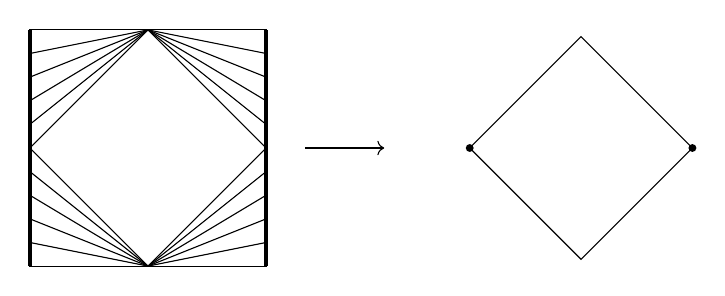
\begin{tikzpicture}
\draw (0,0) rectangle +(3,3);
\draw[ultra thick] (0,0) -- (0,3) (3,0) -- (3,3); 
\foreach \n in {1,...,5}
{
	\draw (1.5,0) -- (0,\n*1.5/5);
	\draw (1.5,0) -- (3,\n*1.5/5);
	\draw (1.5,3) -- (0,3-\n*1.5/5);
	\draw (1.5,3) -- (3,3-\n*1.5/5);
}
\draw[->] (3.5,1.5) -- (4.5,1.5);
\draw[rotate around={45:(7,1.5)}] (6,0.5) rectangle +(2,2);
\fill[rotate around={45:(7,1.5)}] (6,2.5) circle (0.05);
\fill[rotate around={45:(7,1.5)}] (8,0.5) circle (0.05);
\end{tikzpicture}
\end{center}

Here the function is constant on the vertical edges of the square at the two vertices, 
and on each diagonal line as shown maps to the corresponding edges of the square on the 
right.
Thus if $h$ factors through one of $U$ or $V$, $K_1(\gamma_0) = K_1(\gamma_1)$, since 
$[\gamma_0] = [\gamma_1]$ in one of $\Pi_1(U)$, $\Pi_1(V)$.

\lecturenum{12}

By\marginnote{%
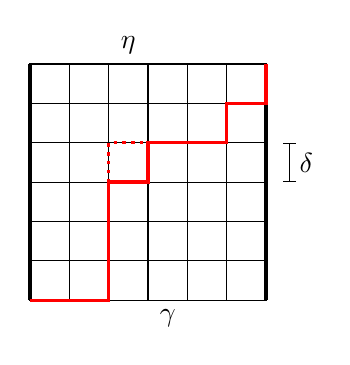
\begin{tikzpicture}
\draw (0,0) rectangle (3,3);
\draw (1.75,0) node[below] {$\gamma$};
\draw (1.25,3) node[above] {$\eta$};
\draw[ultra thick] (0,0) -- (0,3) (3,0) -- (3,3);
\foreach \x in {0,...,5}
{
	\foreach \y in {0,...,5}
	\draw (\x/2,\y/2) rectangle (\x/2+0.5,\y/2+0.5);
}
\draw[|-|] (3.3,1.5) -- node[right] {$\delta$}  (3.3,2);
\draw[very thick,red] (0,0) -- (1,0) -- (1,1.5) -- (1.5,1.5) -- (1.5,2) --
		(2.5,2) -- (2.5,2.5) -- (3,2.5) -- (3,3);
\draw[very thick,red,dotted] (1,1.5) -- (1,2) -- (1.5,2);
\end{tikzpicture}
} the Lebesgue covering lemma applied $(I^2,d_\infty)$ and the open cover 
$\{H^{-1}(U^o), H^{-1}(V^o)\}$, there is a some $\delta > 0$ such that every square of 
side-length $\leq\delta$ in $I^2$ (a \emph{$\delta$-square}) is contained in one of 
$H^{-1}(U^o)$ and $H^{-1}(V^o)$. Thus $H\big|_{[a,a+\delta]\times[b,b+\delta]}$ factors 
through one of $U$ or $V$, for any suitable $(a,b)\in I^2$. We then cover $I^2$ by such 
$\delta$-squares, noting that this also give a partition of $I$ into intervals such that 
both $\gamma$ and $\eta$ restricted to such intervals factor through one of $U$ or $V$, 
so that $K_1$ is defined on $\gamma$ and $\eta$.

Now we can use the fact about paths between opposite vertices of the square 
being\marginnote{all homotopies here will have fixed endpoints} homotopic to iteratively 
show that $K_1(\gamma) = K_1(\eta)$. Firstly, note that $\gamma$ is homotopic to the 
path gotten by concatenating with the constant path up the right side of the square, and 
similarly, $\eta$ is homopic to the path gotten by concatenating with the constant path 
up the left side of the square. Then the big homotopy is pasted together from homotopies 
that move one square at a time, each of which land in one of $U$ or $V$. Then the two 
possible red paths shown in the figure, for example, get mapped by $K_1$ to the same morphism 
in $\Gamma$. All up, these show that $K_1(\gamma) = K_1(\eta)$, and so $K_1$ is 
well-defined on homotopy classes of paths. By the construction of $K_1$, it preserves 
composition, so is functorial, and we are done.
\end{proof}

This is a powerful theorem, but sometimes not the best for computation, in this form. It 
would be good to have a version for more general $\Pi_1(X,A)$, for smaller $A\subset X$, 
or even $\pi_1(X,x)$. To do this, we need a general categorical lemma

Given\marginnote{%
$\xymatrix@!=2ex{
	A_1 \ar[rr] \ar[dd] \ar[dr] && B_1 \ar[dr] \ar[dd]|\hole\\
	& A_2 \ar[rr] \ar[dd] && B_2 \ar[dd]\\
	C_1\ar[dr] \ar[rr]|\hole && D_1\ar[dr] \\
	& C_2 \ar[rr] && D_2
}$\\
\noindent A morphism from the back square to the front square in $\cC^\square$} 
an arbitrary category $\cC$, we can define a category $\cC^\square$ with objects 
commutative squares in $\cC$, and morphisms commutative \emph{cubes}: cubes of objects 
and morphisms such that every face is a commutative square.

\begin{definition}
In a category $\cC$, an object $V$ is a \emph{retract} of an object $W$, if\marginnote{the morphism $r$ is called a \emph{retraction}} there are 
morphisms $i\colon V\to W$ and $r\colon W\to V$ such that $r\circ i = \id_V$.
\end{definition}

For example, in $\Vect$, any subspace $V$ of $\RR^n$ is a retract, by taking $i$ to be 
the inclusion, and $r$ to be orthogonal projection onto $V$. In $\Set$, given a set $S$ 
and a subset $T \subseteq S$ with some chosen $t_0\in T$ we get a retract given by the 
inclusion and the function $r\colon S\to T$ defined by $r(t) = t$, for $t\in T$, $r(s) = 
t_0$ for $s\in S\setminus T$. A more serious example is:
		
\begin{example}\label{eg:retracts_of_Pi1}
Given a space\marginnote{This generalises the case from Assignment 2, where $A'=\{x\}$} 
$X$, with subspaces $A' \subseteq A$ such that every point in $A$ is 
connected by a path in $X$ to a point in $A'$. Then $\Pi_1(X,A')$ is a retract of 
$\Pi_1(X,A)$. The case we will most care about is $A=X$, and various $A'\subseteq X$.
\end{example}

We can talk about what it means for a commutative square in a category $\cC$ to be a 
retract of another commutative square in $\cC$, by looking at retracts in $\cC^\square$. 
Recall that pushout squares are special examples of commutative squares. Also, to check 
that a morphism of commutative squares is a retraction, it is enough to check that it is 
a retraction at each vertex (that is, we have four retractions in $\cC$, one for each 
vertex of the square)

\begin{lemma}\label{lemma:retracts_of_pushouts}
Retracts of pushout squares are pushout squares.
\end{lemma}

\begin{proof}
Exercise.
\end{proof}

We wish to apply Lemma~\ref{lemma:retracts_of_pushouts} to the pushout square in 
$\Gpd$---hence an object of $\Gpd^\square$---from the Seifert--van Kampen theorem, which 
involved fundamental groupoids $\Pi_1(X)$ etc. Retracts (in $\Gpd$) as in 
Example~\ref{eg:retracts_of_Pi1} will be assembled to give a retract in $\Gpd^\square$ that
is made up of smaller and more manageable groupoids.

\begin{theorem}[Relative Seifert--van Kampen theorem]
Let $X$ be a space, $\{U,V\}$ be a cover by nhds, and $A\subseteq X$ a given subspace. 
If in each of the four pairs $(X,A)$, $(U,A\cap U)$, $(V,A\cap V)$, $(U\cap V,A\cap 
U\cap V)$, every point\marginnote{so a point in $U$ is connected by a path in $U$ to a point in $A\cap U$, and so on} in the larger space is connected by a path (in that space) to a point in 
the smaller space, then
\[
\xymatrix{
	\Pi_1(U\cap V,A\cap U\cap V) \ar[r] \ar[d] & \Pi_1(V,A\cap V)\ar[d]\\
	\Pi_1(U,A\cap U) \ar[r] & \Pi_1(X,A)
}
\]
is a pushout square in $\Gpd$.
\end{theorem}

\begin{proof}

The hard work involving homotopies etc is already done, we just need to exhibit the 
square as shown as a retract in $\Gpd^\square$ of the pushout square in the statement of 
the Seifert--van Kampen theorem. By Example~\ref{eg:retracts_of_Pi1}, each of the 
groupoids in the commutative square are, individually, retracts.
The inclusion functors
\begin{align*}
\Pi_1(U\cap V,A\cap U\cap V) & \into \Pi_1(U\cap V)\\
\Pi_1(U,A\cap U) & \into \Pi_1(U)\\
\Pi_1(V,A\cap V) & \into \Pi_1(V)\\
\Pi_1(X,A) & \into \Pi_1(X)
\end{align*}
give a morphism in $\Gpd^\square$, so we just need to construct the functors
\begin{align*}
\Pi_1(U\cap V,A\cap U\cap V) & \leftarrow \Pi_1(U\cap V)\\
\Pi_1(U,A\cap U) & \leftarrow \Pi_1(U)\\
\Pi_1(V,A\cap V) & \leftarrow \Pi_1(V)\\
\Pi_1(X,A) & \leftarrow \Pi_1(X)
\end{align*}
that together give a morphism of commutative squares in the other direction. To do this, 
we will choose, for each $x\in X$, a (homotopy class of a) path $\eta_x\colon 
x\rightsquigarrow a_x$, for some $a_x \in A$, such that if $x\in U$, take $a_x\in A\cap 
U$ and $\eta_x$ a path in $U$; if $x\in V$, take $a_x\in A\cap V$ and $\eta_x$ a path in 
$V$; and hence if $x\in U\cap V$, it follows that $a_x\in A\cap U\cap V$ and $\eta_x$ is 
a path in $U\cap V$. Further, if $x\in A$ already, take $a_x = x$, and $\eta_x$ the 
constant path.

The assignment $x\mapsto a_x$, and $(x\stackrel{\gamma}{\rightsquigarrow} y) \mapsto 
(a_x \rightsquigarrow x \rightsquigarrow y \rightsquigarrow a_y)$ gives a functor 
$\Pi_1(X) \to \Pi_1(X,A)$, and this is a retraction. By the specific choices of $a_x$ 
and $\eta_x$ we made, the restrictions of this functor to the groupoids $\Pi_1(U)$, 
$\Pi_1(V)$, $\Pi_1(U\cap V)$ land in the corresponding subgroupoids $\Pi_1(U,A\cap U)$ 
etc, and again give a retraction in each case. We can check that these do indeed give us 
a morphism in $\Gpd^\square$, which is enough to show we have a retraction in $\Gpd^\square$. 
\end{proof}

We would like to consider pushouts of groups, since these can be easier in some cases to 
compute. The statement of the relative Seifert--van Kampen theorem however involves 
pushouts of groupoids, so that even if we consider one-obect groupoids associated to 
groups we need to be careful that the universal property for the pushout in $\Gpd$ 
implies the universal property for the pushout in $\Grp$. Thankfully, this is true, for 
abstract reasons.

\begin{lemma}
Let $\cC$ be a category and let $\cD \into \cC$ be a full subcategory. Let
\[
\xymatrix{
	A\ar[r] \ar[d] & B \ar[d]\\
	C \ar[r] & P
}
\]
be a commutative square in $\cD$ that is a pushout square in $\cC$. Then it is a pushout
square in $\cC$.
\end{lemma}

\begin{proof}
We will check the universal property for the pushout in $\cC$. Let
\[
\xymatrix{
	A\ar[r] \ar[d] & B \ar[d] \\
	C \ar[r] & D
}
\]
be an arbitrary commutative square in $\cD$. Then considering this as a commutative 
square in $\cC$, we have a unique morphism $k\colon P\to D$ (in $\cD$) compatible with 
the other data as in the definition of pushout square. But since $\cC$ is a \emph{full} 
subcategory, $k$ is a morphism in $\cC$, and moreover the commuting triangles still 
commute in $\cC$. Given any other morphism $P\to D$ in $\cC$ making the triangles commute will
be equal to $k$ in $\cD$, and hence in $\cC$, so the universal property for the pushout
holds in $\cC$.
\end{proof}

Now we can use the fact that $\mathbb{B}\colon \Grp \to \Gpd$ expresses $\Grp$ as a full 
subcategory.

\begin{corollary}
Let $X$ be a path connected space, $\{U,V\}$ a cover by path connected nhds with 
$U\cap V$ path connected. For $x\in U\cap V$, the square
\[
\xymatrix{
	\pi_1(U\cap V,x) \ar[r] \ar[d] & \pi_1(V,x) \ar[d]\\
	\pi_1(U,x) \ar[r] & \pi_1(X,x)
}
\]
is a pushout square in $\Grp$.
\end{corollary}

\begin{proof}
The hypotheses on $X$, $U$, $V$ and $x$ imply that the condition of the relative 
Seifert--van~Kampen theorem hold, so that we have a pushout of one-object groupoids. But 
by the above lemma, we get a pushout of groups.
\end{proof}

So we need to know what pushouts of groups look like!


\begin{example}

Consider the cover of the sphere $S^n$, where $n>1$, by $U=S^n\setminus\{N\}$ and 
$V=S^n\setminus\{S\}$, where $N$ and $S$ are a pair of antipodal points (North and South 
poles). Then $U\cap V \simeq S^{n-1}\times (-1,1)$, and all these spaces are path 
connected, so we can apply the group version of Seifert--van~Kampen. Take a basepoint 
$x\in S^{n-1} \subset U\cap V$. Using stereographic projection, we get that $U\simeq 
\RR^n \simeq V$, hence both of these are contractible, and so $\pi_1(U,x) = 1 = 
\pi_1(V,x)$ are both the trivial group. Then by Seifert--van~Kampen we know that
\[
\xymatrix{
	\pi_1(S^{n-1}\times(-1,1),x) \ar[r] \ar[d] & 1 \ar[d]\\
	1 \ar[r] & \pi_1(S^n,x)
}
\]
is a pushout square. If we take an arbitrary group $K$ then to check the universal 
property, the data of the homomorphisms $1\to K \leftarrow 1$ tells us nothing, the 
compatibility being automatically satisfied, so we need $\pi_1(S^n,x)$ to be a group 
such that there is a \emph{unique} homomorphism from it to $K$. But the only group that 
has a unique homomorphism to any other group is the trivial group. Thus $\pi_1(S^n,x)=1$ 
for all $n>1$.
\end{example}

This argument fails for $n=1$ since the cover as constructed in that case results in the 
intersection $U\cap V$ being the disjoint union of two intervals, so not path connected.

\lecturenum{13}

\begin{definition}

Let $G\xleftarrow{\phi} L \xrightarrow{\psi} H$ be a pair of homomorphisms. The 
\emph{free product with amalgamation} $G\ast_L H$ is the group $G\ast H/\langle 
\phi(x)\psi(x)^{-1}\rangle$, where $\langle \phi(x)\psi(x)^{-1}\rangle$ is the smallest normal 
subgroup generated by the elements $\phi(x)\psi(x)^{-1}$ for all $x\in L$. There are 
homomorphisms $G\to G\ast_L H \leftarrow H$, and $G\ast_L H$ satisfies the universal 
property of the pushout in $\Grp$.

\end{definition}

Note\marginnote{this description also works for groups that aren't finitely presented}
 that if $G = \langle g_1,\ldots,g_m \mid R_1,\ldots,R_n\rangle$ and $H=\langle 
h_1,\ldots,h_k \mid Q_1,\ldots,Q_l\rangle$, then
\[
	G\ast_L H \simeq \langle g_1,\ldots,g_m,h_1,\ldots,h_k\mid R_1,\ldots R_n,Q_1,\ldots, Q_l,
			\phi(x)\psi(x)^{-1}=e \rangle 
\]
where we add a new relation for each $x\in L$, or even just each $x$ running through a 
set of generators for $L$. Note that these relations are equivalent to $\phi(x) = \psi(x)$,
so that we do indeed get a commutative square.

\begin{example}\label{eg:one-relator_group}
Consider a \emph{finitely generated one-relator group}\marginnote{Such groups are important in geometric group theory, and much is known about them} 
$G= \langle g_1,\ldots,g_m\mid R=e\rangle$ ($R$ is an element of the free group generated by $g_1,\ldots,g_m$). Such a group is a pushout of the form
\[
\xymatrix{
	\ZZ \ar[r] \ar[d]_r & 1 \ar[d] \\
	F_m \ar[r] & G
}
\]
where $R = r(1)$.
\end{example}

For a more specific example, take the \emph{surface group}
\[
\langle a_1,\ldots, a_g,b_1,\ldots,b_g\mid \prod_{i=1}^g [a_i,b_i] \rangle.
\]
More generally, one can write a finitely presented group as a pushout
\[
\xymatrix{
	F_n \ar[r] \ar[d]_r & 1 \ar[d] \\
	F_m \ar[r] & \langle g_1,\ldots,g_m\mid r(a_1)=e,\ldots r(a_n)=e\rangle
}
\]
where we take $F_n \langle a_1,\ldots,a_n\mid\ \rangle$.


\begin{rem}
Going back to free products, for a moment, a famous example is the free product $\ZZ/2\ast \ZZ/3$, which is isomorphic to the \emph{modular group} 
\[
	PSL_2(\ZZ) = \{2\times 2 \text{ integer matrices } A\mid \det(A) = 1\}/\{\pm I\}
\]

One presentation\marginnote{It is not obvious that this even is a presentation, for a proof see Roger C. Alperin, $PSL_2(\mathbf{Z}) = \mathbf{Z}_2 \ast \mathbf{Z}_3$, The American Mathematical Monthly Vol. 100, No. 4 (Apr., 1993), pp. 385--386, doi:10.2307/2324963}
 of $PSL_2(\ZZ)$ is via the generators $S=\begin{psmallmatrix}0&-1\\1&0 
\end{psmallmatrix}$ and $ST = \begin{psmallmatrix}1 &-1 \\1 &0 \end{psmallmatrix}$, 
which satisfy $S^2=I$ and $(ST)^3=I$. Note that $PSL_2(\ZZ)$ acts by fractional linear 
transformations on the upper half plane $\mathcal{H} = \{z\in \CC \mid Im(z) > 0\}$, 
with $S\colon z \mapsto \frac{-1}{z}$ and $ST\colon z\mapsto \frac{1-z}{z}$. This action 
is continuous and has discrete orbits, and this is enough to make $\mathcal{H} \to 
\mathcal{H}/PSL_2(Z)$ a covering space.
\end{rem}

Give the concrete treatment for the pushout of groups above (that is, as free products 
with amalgamation), one could hope for a similar treatment for groupoids. And indeed, 
one can do this, where instead of group elements being (equivalence classes of) words in 
the elements of the given groups, morphisms of the pushout groupoid are (equivalence 
classes of) words in the morphisms of the given groupoids. However, we need to be 
careful about what we mean by words constructed as a string of morphisms, since not all 
morphisms can be composed.

We will not give the most general treatment here, but show how to describe the pushout 
of groupoids in a special case corresponding to a situation arising from an application 
of the Seiert--van~Kampen theorem.

\begin{example}

Let $X$ be a space, $\{U,V\}$ a cover by nhds, and $A\subseteq U\cap V$ be such that 
every path component of $U$, $V$ and $U\cap V$ contains at least one point in $A$. Then 
we can apply the Seifert--van~Kampen theorem and get a pushout square
\[
\xymatrix{
	\Pi_1(U\cap V,A) \ar[r]^{i_V} \ar[d]_{i_U} & \Pi_1(V,A) \ar[d]\\
	\Pi_1(U,A) \ar[r] & \Pi_1(X,A)
}
\]
Note that all four groupoids have the same set of objects, and that all 
the functors are the identity on objects (that is: $i_U(a) = a$ and so on). 
From the proof of the Seifert--van~Kampen theorem recall that we expressed paths in $X$,
that is, morphisms in $\Pi_1(X)$ as a composite of paths alternating between $U$ and $V$.
This is the setup we are interested in calulating in general from a purely algebraic point 
of view. For simplicity, we will just think about the case of $A$ finite, which is the case that turns up in calculations of `reasonable' examples.
\end{example}

Suppose we are given a diagram\marginnote{here $H$ is the capital $\eta$}
\[
\xymatrix{
	\Lambda \ar[r]^F \ar[d]_G & H  \\
	\Gamma 
}
\]
in $\Gpd$, where all the groupoids have the same finite set $A = \{a_1,\ldots,a_N\}$ of 
objects, and such that the object components of the functors $F$ and $G$ are all the identity 
function. We wish to construct a groupoid $\Gamma\ast_\Lambda H$ that makes this into a 
pushout square. Firstly, we can take the set of objects to be $A$ again, and the 
functors $\Gamma \to \Gamma\ast_\Lambda H \leftarrow H$ will have as object component 
the identity function.

Given any groupoid\marginnote{and indeed any category} there is a directed graph with 
nodes the objects of the groupoid, and as directed edges the morphism (and we are 
allowed edges from a node to itself, and multiple edges between nodes). And given our 
two groupoids $\Gamma$ and $H$, we can form a graph $\mathcal{G}$ with set of 
nodes $A$, and the directed edges are the \emph{disjoint union} of the morphisms of 
$\Gamma$ (coloured blue) and $H$ (coloured red), and with the identity morphisms removed.
We also don't need to include both a morphism and its inverse, since the inverse can be gotten by traversing a directed edge against the indicated direction.
\begin{center}
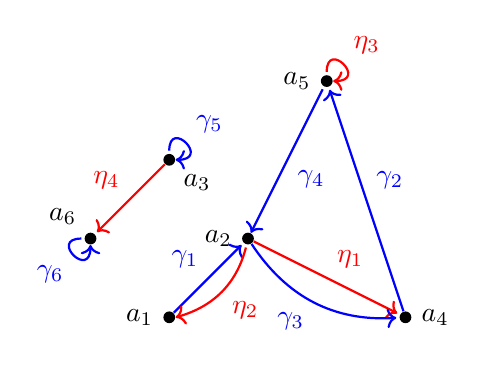
\begin{tikzpicture}
	[object/.style={circle,fill=black,minimum size=1mm,inner sep=1.5pt},
	 bluearrowpre/.style={->,shorten <=1pt,thick,blue},
	 redarrowpre/.style={->,shorten <=1pt,thick,red},
	 bluearrowpost/.style={<-,shorten <=1pt,thick,blue},
	 redarrowpost/.style={<-,shorten <=1pt,thick,red}];
\node[object,label={west:$a_1$}] (a1) at (0,0) {};
\node[object,label={west:$a_2$}] (a2) at (1,1) {}
	edge [bluearrowpost] node[auto,swap] {$\gamma_1$} (a1)
	edge [redarrowpre,bend left] node[auto] {$\eta_2$} (a1.east);
\node[object,label={south east:$a_3$}] (a3) at (0,2) {};
\node[object,label={east:$a_4$}] (a4) at (3,0) {}
	edge [redarrowpost] node[auto,swap] {$\eta_1$} (a2) 
	edge [bluearrowpost,bend left] node[auto] {$\gamma_3$}(a2);
\node[object,label={west:$a_5$}] (a5) at (2,3) {}
	edge [bluearrowpost] node[auto] {$\gamma_2$} (a4)
	edge [bluearrowpre] node[auto] {$\gamma_4$} (a2);
\node[object,label={north west:$a_6$}] (a6) at (-1,1) {}
	edge [redarrowpost] node[auto] {$\eta_4$}(a3);

\draw[bluearrowpre] (a3) to [out=90,in=0,loop,looseness=10] node[auto] {$\gamma_5$} (a3);
\draw[redarrowpre] (a5) to [out=90,in=0,loop,looseness=10] node[auto] {$\eta_3$} (a5);
\draw[bluearrowpre] (a6) to [out=180,in=-90,loop,looseness=10] node[auto,swap] {$\gamma_6$} (a6);
\end{tikzpicture}
\end{center}
Now\marginnote[-4cm]{in the graph shown, composites of various morphisms are omitted, 
for instance ${\color{blue}\gamma_3\gamma_1\gamma_2}$} instead of a word in group 
elements, as in the pushout of groups, we take a \emph{path} in this directed graph, 
alternating between edges that come from $\Gamma$ and edges that come from $H$. For 
instance, we could take
\[
	{\color{blue}\gamma_3^{-1}}{\color{red}\eta_1}{\color{blue}\gamma_2}{\color{red}(\eta_3)^5}{\color{blue}\gamma_4}\qquad\text{or}\qquad 
	{\color{red}\eta_4}{\color{blue}(\gamma_6)^{-3}}{\color{red}\eta_4^{-1}}
\]
from the above graph. The `empty' path consisting just of an identity arrow is also an 
option. However, we haven't yet actually constructed $\Gamma\ast_\Lambda H$, merely what 
we might call $\Gamma \ast_{\Lambda_0}H$,\marginnote{if $\Lambda$ is already trivial in 
this sense, then we are done; this is the analogue of the free product of groups} which 
is the pushout where the groupoid $\Lambda$ is replaced by the trivial groupoid 
$\disc(\Lambda_0)$ with the same objects but only identity arrows. What we need to do is 
add `relations', namely extra equalities between morphisms in $\Gamma 
\ast_{\Lambda_0}H$. What this means is that for each morphism $\lambda$ in $\Lambda$, we 
identify the morphisms ${\color{blue}F(\lambda)}$ and ${\color{red}G(\lambda)}$, or more 
precisely, quotient by the equivalence relation on each hom-set of $\Gamma 
\ast_{\Lambda_0}H$ generated by these identifications. For instance, if in the above 
graph, $\gamma_1=F(\lambda_1)$ and $\eta_1 = G(\lambda_1)$, then we add the equality 
$\gamma_1=\eta_1$. This would have the effect of making
\[
	{\color{blue}\gamma_3}{\color{red}\eta_1}{\color{blue}\gamma_2}{\color{red}(\eta_3)^5}{\color{blue}\gamma_4^{-1}} = 
	{\color{blue}(\gamma_3\gamma_1\gamma_2)}{\color{red}(\eta_3)^5}{\color{blue}\gamma_4^{-1}}	
\]
Concatenation of strings and simplifying is the composition in ${\Gamma\ast_\Lambda H}$.

\begin{ex}
Prove that this construction makes $\Gamma\ast_\Lambda H$ a groupoid.
\end{ex}

If we are interested in merely looking at the group of morphisms from a single object $a_i$ to itself,
which is the case when calculating a fundamental group using the groupoid Seifert--van~Kampen,
then we should look at paths that start and finish at the chosen $a_i$.


\begin{example}

Let us look at an example, arising from an application of Seifert--van~Kampen. Consider 
the circle $S^1$ as sitting in $\CC$, and let $U=S^1\setminus \{-i\}$, $V=S^1\setminus 
\{i\}$. All three of these are path connected, and let us take $A={+1,-1} \subset U\cap 
V$. This choice of data satisfies the hypotheses of SvK. The pushout square
\[
\xymatrix{
	\Pi_1(U\cap V,\{\pm1\}) \ar[r] \ar[d] & \Pi_1(V,\{\pm1\}) \ar[d]\\
	\Pi_1(U,\{\pm1\}) \ar[r] & \Pi_(S^1,\{\pm1\})
}
\]

can be simplified as follows. First, $U \simeq (-2,2) \simeq V$, in a way that preserves 
$A=\{\pm1\}$, so that 
\[
\Pi_1(U,\{\pm1\})  \simeq \mathbf{2} = (-1 \stackrel[\gamma^{-1}]{\gamma}{\leftrightarrows} +1)
\qquad \Pi_1(V,\{\pm1\})  \simeq \mathbf{2} = (-1 \stackrel[\eta]{\eta^{-1}}{\leftrightarrows} +1)
\]
and we have omitted the identity arrows. Here $\gamma$ is a path that runs anticlockwise around $S^1$ from $+1$ to $-1$, and $\eta$ is a path that runs anticlockwise from $-1$ to $+1$.
Second, $\Pi(U\cap V,\{\pm1\}) = \disc(\{+1,-1\})$, so
we are in the easier situation as first outlined above, where no additional quotient needs
to be done. The pushout then looks like
\[
\xymatrix{
*+[F]{-1\phantom{\leftrightarrows}+1} \ar[r] \ar[d] 
& 
*+[F]{-1 {\color{red}\stackrel[\eta]{\eta^{-1}}{\leftrightarrows}} +1}\ar[d] 
\\
*+[F]{-1 {\color{blue}\stackrel[\gamma^{-1}]{\gamma}{\leftrightarrows}} +1} \ar[r] &
\Pi_1(S^1,\{\pm1\})
}
\]
The graph we need so as to generate $\Pi_1(S^1,\{\pm1\})$ is then
\begin{center}
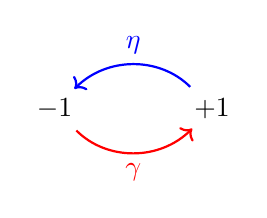
\begin{tikzpicture}
[object/.style={circle,fill=black,minimum size=0.3mm},
	 bluearrow/.style={->,shorten <=1pt,thick,blue},
	 redarrow/.style={->,shorten <=1pt,thick,red}];
\node (plusone) at (0,0) {$-1$};
\node (minusone) at (2,0) {$+1$};

\draw[bluearrow] (minusone) to [out=135,in=45] node[auto,swap] {$\eta$}  (plusone) ;
\draw[redarrow] (plusone) to [out=-45,in=-135] node[auto,swap] {$\gamma$} (minusone) ;

\end{tikzpicture}
\end{center}

Then if we wish to consider paths from $+1$ to itself, the only options are the empty 
path, hence the identity arrow, or $(\eta\gamma)^n$, or $(\gamma^{-1}\eta^{-1})^n = 
(\eta\gamma)^{-n}$. Thus $\pi_1(S^1,+1) \simeq \ZZ$.
\end{example}

\begin{ex}
Prove that this construction of $\Gamma\ast_\Lambda H$ is indeed the pushout in $\Gpd$!
\end{ex}

We will consider one more variant of Seifert--van~Kampen, and this time in brief, 
because the details are similar to other versions. If we would like to compute the 
fundamental group of a join, then it is not quite enough to just consider the free 
product of the fundamental groups: a join does not automatically come with a cover of 
the sort we need for SvK. In what follows, assume: $(X,x)$, $(Y,y)$ are pointed spaces 
such that there exist nhds $x\in U\subseteq X$ and $y\in V\subseteq Y$ that are 
contractible\marginnote{this implies $U\vee V$ is contractible to the basepoint 
$\ast=[x]=[y]$} to $x$ and $y$ respectively, with the contraction fixing the basepoint. 
Then $\{X\vee V, U\vee Y\}$ is a cover of $X\vee Y$ by nhds. We have retractions $X\vee 
V \to X$ and $U\vee Y \to Y$ that preserve the basepoints and which are also homotopy 
equivalences. Thus $\pi_1(X\vee V,\ast)\simeq \pi_1(X,x)$ and $\pi_1(U\vee Y,\ast) 
\simeq \pi_1(Y,y)$, and $\pi_1(U\vee V,\ast)$ is trivial. If we apply the 
Seifert--van~Kampen theorem to the pushout square
\[
\xymatrix{
	(U\vee V,\ast) \ar[r] \ar[d] & (U\vee Y,\ast) \ar[d] \\
	(X\vee V,\ast) \ar[r] & (X\vee Y,\ast)
}
\]
then we get a pushout square of groups
\[
\xymatrix{
	1 \ar[r] \ar[d] & \pi_1(Y,y) \ar[d] \\
	\pi_1(X,x) \ar[r] & \pi_1(X\vee Y,\ast)
}
\]
or in other words, 
\[
	\pi_1(X\vee Y,\ast) = \pi_1(X,x) \ast \pi_1(Y,y).
\]
This generalises the fact that $\pi_1(S^1\vee S^1,\ast) = F_2 = \ZZ\ast \ZZ$ to more 
general spaces.

\begin{fact}
Given any presentation $G=\langle g_1,\ldots,g_m\mid R_1=e,\ldots,R_n=e\rangle$ there is a space
$X$ arising as a pushout\marginnote{$\bigvee_{j=1}^mS^1 = \underbrace{S^1\vee \ldots \vee S^1}_{m\text{ times}}$}
\[
\xymatrixnocompile{
	\bigsqcup_{i=1}^n S^1 \ar[r] \ar[d]_{\langle f_1,\ldots,f_n\rangle} 
		& \bigsqcup_{i=1}^n D^2 \ar[d]\\
	\bigvee_{j=1}^m S^1 \ar[r] & X
}
\]
where $f_i(1)=R_i$, with the property that $\pi_1(X,\ast)\simeq G$. This space is in some 
sense 2-dimensional as it is gotten by gluing together 2d discs, and sometimes a manifold, though not always.

Even better, for \emph{any} group $G$ with any presentation, there is an appropriate pushout
\[
\xymatrixnocompile{
	\bigsqcup_{\beta \in J} S^1 \ar[r] \ar[d]_{\langle f_\beta\rangle} 
		& \bigsqcup_{\beta \in J} D^2 \ar[d]\\
	\bigvee_{\alpha\in I} S^1 \ar[r] & X
}
\]
with the property that $\pi_1(X,\ast) \simeq G$. One has to be careful with the 
topology, and we haven't defined infinite joins,\marginnote{the coutable join 
$\bigvee_{n\in \NN}S^1$ may seem like the Hawaiian earring, but it is in fact not 
compact, and \emph{is} slsc, so they cannot be homeomorphic} but it does work out that 
$\pi_1(\bigvee_{\alpha\in I}S^1,\ast) \simeq F_I$, the free group on the set $I$.
\end{fact}

\begin{example}
An oriented compact Riemann surface $\Sigma_g$ of genus $g\geq 1$ is an example of a 
 surface gotten by a construction as in the Fact above, and even better: it only 
 requires one copy of $D^2$. For genus $g$, it requires doing a pushout of the form
\[
\xymatrixnocompile{
	S^1 \ar[d] \ar[r] & D^2 \ar[d] \\
	\bigvee_{i=1}^{2g} S^1 \ar[r] & \Sigma_g
}
\]
An alternative way to build this pushout is to consider a $4g$-gon,\marginnote{Insert 
octagon picture for case $g=2$ here} and selectively identify edges in pairs (recovering the 
$2g$ circles as in the pushout). The pattern of identifications is exactly that which 
gives rise to the one-relator group after Example~\ref{eg:one-relator_group}, since the 
\emph{attaching map} $S^1 \to \bigvee_{i=1}^{2g} S^1$ in the preceeding pushout is given 
by $\prod_{i=1}^g[a_i,b_i]$, for $a_i$ and $b_i$ the generators of the $2i-1$th and 
$2i$th copy of $S^1$ respectively.
\end{example}

\section{Classifying covering spaces}

Recall\lecturenum{14}
 that for a covering space $Z\xrightarrow{\pi} X$ we get a representation 
\begin{align*}
\rho_Z\colon \Pi_1(X)& \longrightarrow \Set \\
x & \mapsto Z_x\\
[\gamma\colon x\rightsquigarrow y] & \mapsto \left(\gamma_*\colon Z_x\xrightarrow{\simeq} Z_y\right)
\end{align*}

of the fundamental\marginnote{$\xymatrix{Z_1 \ar[rr]^f \ar[dr]_{\pi_1} && Z_2 
\ar[dl]^{\pi_2}\\ & X}$} groupoid of $X$. Given a pair of covering spaces $Z_1,Z_2\to X$ 
and a map between them in $\Cov_X$, how are the representations $\rho_{Z_1}$ and 
$\rho_{Z_2}$ related? Since the triangle at right commutes, we get for each $x\in X$ a 
function between the corresponding fibres, $f\big|_x \colon (Z_1)_x \to (Z_2)_x$. Notice 
that this is a function $\rho_{Z_1}(x) \to \rho_{Z_2}(x)$ for each object of $\Pi_1(X)$. 
Given a path $\gamma\colon x\rightsquigarrow y$ in $X$ and $z\in (Z_1)_x$, we have the 
unique lift to $Z_1$ starting at $z$, namely $\widetilde{\gamma_z}^1\colon 
z\rightsquigarrow \gamma_*(z)$. By composing with $f$, we get a path $f\circ 
\widetilde{\gamma_z}^1\colon I \to Z_2$ from $f(z)$ to $f(\gamma_*(z))$. But by 
uniqueness of lifts of paths, this is the lift of $\gamma$ 
to $Z_2$ starting at $f(z)$, which is a path from $f(z) \rightsquigarrow \gamma_*(f(z))$.
We thus get $f(\gamma_*(z)) = \gamma_*(f(z))$ for every $z\in (Z_1)_x$, implying that the
following square commutes:
\[
\xymatrix{
	(Z_1)_x \ar[r]^{\gamma_*}  \ar[d]_{f\big|_x} &  (Z_1)_y \ar[d]^{f\big|_y} \\
	(Z_2)_x \ar[r]_{\gamma_*} & (Z_2)_y
}
\]
Or, in other words, the functions $f\big|_x$ define a natural transformation 
$\rho_{Z_1}\Rightarrow \rho_{Z_2}$. This leads us to

\begin{prop}
The mapping $(Z \xrightarrow{\pi} X) \mapsto \rho_Z$\marginnote{Recall that the category $[\cC,\Set]$ has as objects the functors $\cC\to \Set$, and as morphisms the natural transformations} define a functor
\[
	\Cov_X \longrightarrow [\Pi_1(X),\Set].
\]
\end{prop}

\begin{proof}
The natural transformation $\rho_Z \Rightarrow \rho_Z$ associated to the identity map 
$Z\to Z$ has a components the identity functions $Z_x\to Z_x$, hence is the identity 
natural transformation. Also, using uniqueness of path lifting one can show that given 
two composable maps of covering spaces, we get functoriality.
\end{proof}

\begin{example}

Regard $S^1\subset \CC$. Recall the covering spaces $\exp(2\pi i(-))\colon \RR \to S^1$ and $S^1 
\xrightarrow{(-)^n} S^1$, for $n>1$. There is a map of covering spaces
\[
\xymatrix{
\RR \ar[rr]^{\exp(2\pi i(-)/n)} \ar[dr]_{\exp(2\pi i(-))} && S^1 \ar[dl]^{(-)^n} \\
& S^1
}
\]
The fibres of $\RR \to S^1$ are isomorphic to $\ZZ$, and indeed the fibre over $1\in 
S^1$ \emph{is} $\ZZ$. The fibre over $1$ of $S^1 \to S^1$ is $\ZZ/n$, and we get the induced map
\begin{align*}
	\ZZ&\to \ZZ/n\\
	k & \mapsto k \pmod{n}
\end{align*}

Now note that if we focus on the point $1\in S^1$, then a morphism in $\Pi_1(S^1)$ from 
$1$ to itself is the homotopy class of some loop, which can identify with an integer 
under $\pi_1(S^1,1) \simeq \ZZ$. Then the representation associated to $\RR\to S^1$ is
\begin{align*}
\rho_\RR\colon \Pi_1(S^1)& \longrightarrow \Aut(\ZZ) \\
m &\mapsto (k\mapsto k+m)
\end{align*}
whereas the representation associated to $(-)^n\colon S^1\to S^1$ is
\begin{align*}
\rho_n\colon \Pi_1(S^1)& \longrightarrow \Aut(\ZZ/n)\simeq S_n \\
m &\mapsto (k\mapsto k+m \pmod{n})
\end{align*}
The map $\ZZ\to \ZZ/n$ is clearly equivariant for the shift action of $\ZZ$ as shown, as 
a special case of the naturality of the map $\ZZ\to \ZZ/n$.
\end{example}


\begin{q}
What representations $\Pi_1(X) \to \Set$ can arise as $\rho_Z$ for some covering space $Z\to X$?
\end{q}

Recall that it is obvious that every set is the set of connected components of some 
space, and while we didn't go into details, the construction of a space $X$ with 
$\pi_1(X,\pt)\simeq G$ for any given $G$ is a relatively uncomplicated pushout. However, 
given a representation $\Pi_1(X) \to \Set$, it is not immediately obvious how to build a 
covering space giving rise to it. Indeed, all the covering spaces we have seen so far 
are either natural examples we happen to have seen, or special toy cases chosen to 
illustrate some small aspect of the fundamental groupoid of a particularly simple space. 
We are going to look at doing some reductions to simpler cases, on both sides (the 
topological, $\Cov_X$ and the algebraic, $[\Pi_1(X),\Set]$) to make the task easier.

First, since we have the blanket assumption that out spaces are slpc, we can consider 
finding a section to the continuous map $X\to [\pt,X]$, namely $A\colon [\pt,X] \to X$, 
that picks out one point $a_i$ per path component $X_i \subseteq X$. We have the full 
subgroupoid inclusion $\Pi_1(X,A) \into \Pi_1(X)$ that is additionally an 
equivalence.\marginnote{by an argument as in the solutions for assignment 2, question 7} 
Let us denote by $I$ the set $[\pt,X]$ in what follows.

\begin{lemma}
If $i\colon \cC\into \cD$ is a full subcategory inclusion that is also an equivalence, then 
the restriction map
\begin{align*}
[\cD,\Set]& \xrightarrow{i^*} [\cC,\Set]\\
F & \mapsto F\circ i
\end{align*}
is an equivalence of categories.
\end{lemma}

\begin{proof}
Exercise.
\end{proof}

Now notice also that $\Pi_1(X,A) = \Pi_1(\bigsqcup_{i\in I}X_i,\bigsqcup_{i\in I}\{a_i\}) \simeq \bigsqcup_{i\in I} \mathbb{B}\pi_1(X_i,a_i)$

\begin{lemma}
For any family of categories $(\cC_i)_{i\in I}$ we have an isomorphism\marginnote{An object of a product of family of cateories is a tuple of objects, one from each of the categories, and similar with the morphisms}
\[
	[\bigsqcup_{i\in I} \cC_i,\Set] \xrightarrow{\simeq} \prod_{i\in I}[\cC_i,\Set]. 
\]
\end{lemma}

\begin{proof}
Exercise.
\end{proof}

Given a group $G$, we can define the category $G\Set$ which has as objects sets $S$ 
equipped with a $G$-action, $G\to \Aut(S)$, and with morphisms \emph{equivariant} 
functions.\marginnote{An equivariant function $f\colon S\to T$ satisfies $f(g\cdot p) = 
g\cdot f(p)$ for all $p\in S$} Note that for any groupoid $\Gamma$ and representation 
$\rho\colon \Gamma \to \Set$, for each object $x\in \Gamma_0$ there is a permutation 
representation $\Gamma(x,x) \to \Aut(\rho(x))$. To any natural transformation 
$\rho\Rightarrow \rho'$ between representations, there is an equivariant map between 
$\Gamma(x,x)$-sets, and this is functorial.

\begin{lemma}
The functor just described gives an isomorphism $[\mathbb{B}G,\Set] \xrightarrow{\simeq} G\Set$ of categories
\end{lemma}

We can put all of these lemmas together and get an equivalence of categories
\[
[\Pi_1(X),\Set] \to [\Pi_1(X,A),\Set] \simeq \prod_{i\in I}[\mathbb{B}\pi_1(X_i,a_i),\Set]
\simeq \prod_{i\in I}\pi_1(X_i,a_i)\Set.
\]
We can compose this with the original functor we were looking at, from covering spaces to representations, to get
\begin{align}
	\Cov_X & \to \prod_{i\in I}\pi_1(X_i,a_i)\Set \label{eq:fibre_functor}\\
	(Z\to X) & \mapsto (\rho_i\colon \pi_1(X_i,a_i) \to Z_{a_i})_{i\in I} \nonumber
\end{align}
where now the codomain is much more tractable. Further, the objects in categories of the 
form $G\Set$ are not unreasonable: we can break them down into smaller parts. Each 
object $\rho\colon G\to \Aut(S)$ in $G\Set$ isomorphic to one of a particularly nice 
form, namely $S\simeq \bigsqcup_{j\in S/G} G/\mathrm{Stab}(p_j)$, where the points 
$p_j\in S$ are chosen so that there is one in each orbit of the $G$-action.

\begin{rem}
From now on, we will consider only spaces that are slsc, since this will ultimately be 
the case in the classification theorem, and also because $X$ slsc implies that for every 
covering space $Z\to X$, the space $Z$ is locally path connected, so that path 
components and components agree.
\end{rem}

\lecturenum{15}
\begin{lemma}
For a space $X = \bigsqcup_{i\in I} X_i$, there is an equivalence of categories $\Cov_X \simeq \prod_{i\in I} \Cov_{X_i}$.
\end{lemma}

\begin{proof}
A covering space $Z\to \bigsqcup_{i\in I} X_i$ gives covering spaces $Z_{X_j}:=\mathrm{in}_j^*X$ for each $j\in I$, where recall the inclusion maps $\mathrm{in}_j\colon X_j \to \bigsqcup_{i\in I} X_i$. We also get, from a map of covering space $Z\to Z'$ over $X$, a map $Z_{X_j} \to Z'_{X_j}$ of covering spaces over $X_j$, for each $j$. This gives a functor $\Cov_X \to \prod_{i\in I} \Cov_{X_i}$.

Conversely, given a covering space $Z_i \to X_i$ for each $i\in I$, we get a covering space $\bigsqcup_{i\in I} Z_i \to \bigsqcup_{i\in I} X_i$, and for maps $Z_i \to Z'_i$ of covering spaces over $X_i$, there is a map $\bigsqcup_{i\in I} Z_i \to \bigsqcup_{i\in I} Z'_i$ of covering spaces over $\bigsqcup_{i\in I}X_i$. This gives a functor $\prod_{i\in I} \Cov_{X_i} \to \Cov_X$, and these two functors are an equivalence of categories.
\end{proof}

The functor in (\ref{eq:fibre_functor}) then factorises as the composite
\begin{align*}
	\Cov_X & \xrightarrow{\simeq} \prod_{i\in I} \Cov_{X_i} \longrightarrow \prod_{i\in I}\pi_1(X_i,a_i)\Set\\
	\raisebox{4ex}{\xymatrix{Z\ar[d]\\X}} & \mapsto 
	\raisebox{4ex}{\xymatrix{Z_{X_i}\ar[d]\\X_i} } \mapsto 
	\left(\rho_i\colon \pi_1(X_i,a_i) \to \Aut(Z_{a_i}) \right)
\end{align*}
In particular, if we understand each $\Cov_{X_i} \to\pi_1(X_i,a_i)\Set$, then we are done. 

So, we will consider from now on the case of a connected, slsc space $X$ with chosen $x_0\in X$, and the functor $\Cov_{X} \to\pi_1(X,x_0)\Set$. 

Since $X$ is slsc, it is locally path connected, and the local trivialisation of any covering space $Z\to X$ shows that $Z$ is also locally path connected.\marginnote{there is a small subtlety here, in that we really require a basis of nhds that are path connected, I will expand on this point if pushed, but it is a technicality that can be ignored for our purposes} We can then write $Z = \bigsqcup_{\alpha \in I} Z_\alpha \to X$, where each $Z_\alpha \to X$ is a (path) connected covering space.\marginnote{Exercise!}

\begin{example}
Take $X=S^1$. Recall that we have various covering spaces: $S^1\times F\simeq \bigsqcup_{F} S^1\to S^1$ for discrete spaces $F$; the exponential map $\RR \to S^1$; the various $S^1 \xrightarrow{(-)^n} S^1$ with $n>1$, where we shall write $S^1_n$ for the total space of this covering space. Then we can form a covering space
\[
	S^1\times F \sqcup \bigsqcup \RR \sqcup \bigsqcup S^1_2 \sqcup \bigsqcup S^1_3\sqcup \ldots \to S^1.
\]
It remains to be seen, however, if there are any covering spaces not of this form.
\end{example}

Recall from lecture 6 (on page~\pageref{eq:fibre_quotient_of_loops}) that given a covering space $Z\to X$, there is a surjective map
\[
	\Omega_{x_0} X \times\{z_\alpha\mid \alpha \in I\} \to Z_{x_0}, \qquad z_\alpha \in Z_{x_0}\cap Z_\alpha,
\]
hence a surjective map \[
	\pi_1(X,x_0) \times \{z_\alpha\mid \alpha \in I\} \simeq \bigsqcup_{\alpha\in I}\pi_1(X,x_0) \times  \{z_\alpha\} \to Z_{x_0} = \bigsqcup_{\alpha\in I} Z_{x_0}\cap Z_\alpha
\]
\begin{lemma}
Given a covering space $Z\to X$ with $x_0\in X$, then $Z_{x_0} =\bigsqcup_{\alpha\in I} Z_{x_0}\cap Z_\alpha\simeq \bigsqcup_{\alpha\in I} \pi_1(X,x_0)/\pi_1(Z_\alpha,z_\alpha)$ as $\pi_1(X,x_0)$-sets, for any choice of $z_\alpha\in Z_{x_0}\cap Z_\alpha$.
\end{lemma}

\begin{proof}
It is enough to show that the orbits of the $\pi_1(X,x_0)$-action are the sets $Z_{x_0}\cap Z_\alpha$, because then the general description of sets with transitive action takes over. Given $z\in Z_{x_0}\cap Z_\alpha$, there is a path $\gamma\colon z_\alpha \rightsquigarrow z$, and hence a loop $\pi\circ\gamma$ at $x_0$. This loop acts on $Z_{x_0}$, with $(\pi\circ \gamma)_*(z_\alpha)=z$. Hence $Z_{x_0}\cap Z_\alpha$ is contained in the orbit containing $z_\alpha$. Conversely, given any $z\in Z_{x_0}$ and a loop $\eta$ at $x_0$ such that $\eta_*(z_\alpha) = z$, then there is a lift $\widetilde{\eta}\colon z_\alpha \rightsquigarrow z$ of $\eta$, so that $z\in Z_\alpha$. Thus the orbit of $z_\alpha$ is contained in $Z_{x_0}\cap Z_\alpha$, and we are done.
\end{proof}

As a result, our functor $\Cov_X \to \pi_1(X,x_0)\Set$ preserves disjoint unions: it sends the covering space $\bigsqcup_{\alpha \in I} Z_\alpha\to X$ to the disjoint union of sets with a permutation representation $\bigsqcup_{\alpha\in I} Z_{x_0}\cap Z_\alpha$.

\begin{rem}
Given a group $G$ and a $G$-set $S$, such that $S=\bigsqcup_{\alpha\in I} S_\alpha$ is the partition into orbits of the action, then the representation $\rho \colon G\to \Aut(\bigsqcup S_{\alpha\in I})$ factors through the subgroup $\prod_{\alpha\in I} \Aut(S_i) < \Aut(\bigsqcup S_{\alpha\in I})$, hence $\rho = (\rho_\alpha)_{\alpha\in I}$, for $\rho_\alpha\colon G\to \Aut(S_\alpha)$ a transitive $G$-action.
\end{rem}

Recall what our original question was: what representations $\Pi_1(X)\to \Set$ arise from covering spaces of $X$ via the functor $\Cov_X \to [\Pi_1(X),\Set]$? We have now reduced this to the simpler aim of starting with a permutation representation of a fundamental group, and can reduce the input data even more. Inside $\Cov_X$ (for connected $X$) is the full subcategory $\Cov_X^\mathrm{conn}$ of \emph{connected} covering spaces, and inside $\pi_1(X,x_0)\Set$ is the full subcategory $\pi_1(X,x_0)\Set^\mathrm{tr}$ of sets with a \emph{transitive} action. Moreover, in both of these cases, arbitrary objects in $\Cov$ and $\pi_1(X,x_0)\Set$ can be gotten by disjoint union of objects in the respective subcategories. Thus it is sufficient to ask if we can get any transitive $\pi_1(X,x_0)$-set from some connected covering space of $X$. That is, we want to know what is the image of the functor
\[
	\Cov_X^\mathrm{conn} \longrightarrow  \pi_1(X,x_0)\Set^\mathrm{tr}.
\]

Note that in the category of transitive $G$-sets, every object $S$ with a point $p\in S$ is the quotient of the underlying set of $G$ equipped with the action by multiplication, via the map 
\begin{align*}
G& \to S \simeq G/\mathrm{Stab}(p)\\
g & \mapsto g\cdot p
\end{align*}
and the $G$-action on $G$ is free and transitive. More generally, given any $G$-set $T$ with a free and transitive action, there is a surjective equivariant map $T\to S$ displaying $S$ as a quotient of $T$.

\begin{example}
Given a simply-connected covering space $Z\to X$ and $x_0\in X$, the fibre $Z_{x_0}$ is a free and transitive $\pi_1(X,x_0)$-set.
\end{example}

Recall also that for a general path connected covering space $Z\to X$, $Z_{x_0} \simeq \pi_1(X,X_0)/\pi_1(Z,z)$ for any $z\in Z_{x_0}$. If we start with a pointed covering space, then we don't have to choose a point, and every connected covering space of a pointed space can be gotten by forgetting the point from some pointed covering space.
So we have the final form of the question

\begin{q}
Given a subgroup $H< \pi_1(X,x_0)$, is there a pointed covering space $(Z,z_0)\to (X,x_0)$ such that $\pi_1(Z,z_0) = H$ as subgroups of $\pi_1(X,x_0)$?\marginnote{Recall from assignment 2, where from a simply-connected space $Y$ with free $G$-action, we got a covering space $Y\to Y/G$ with $\pi_1(Y/G,\ast)\simeq G$}
\end{q}


Recall\lecturenum{16} that for a simply-connected covering space $Z^{(1)} \to X$ the fibre over $x_0$ is isomorphic to $\pi_1(X,x_0)$, and that our ultimate aim is to get a covering space with fibre isomorphic to $\pi_1(X,x_0)/H$. So one way to approach this is to see if there is a way to make sense of making a covering space by taking the quotient of some simply-connected covering space ``fibre by fibre''. It isn't possible to do this piecemeal, so we need to do this for all fibres at once.

\begin{definition}
Let $p\colon Y\to X$ be a map of spaces, $G$ a group acting on $Y$. We say the action is \emph{fibrewise} if $p(g\cdot y) = p(y)$ for all $y \in Y,g\in G$.
\end{definition}

It follows from the definition\marginnote{there is a commutative triangle $\xymatrix{Y \ar[d] \ar[r] & Y/G \ar[dl]\\ X}$} that there is map $Y/G \to X$, and the fibre of this map over $x$ is $p^{-1}(x)/G$.

\begin{prop}
Let $Z\xrightarrow{\pi} X$ be a covering space, and let $G$ act fibrewise on $Z$. Then $Z/G\to X$ is a covering space and $Z\to Z/G$ is a map of covering spaces.
\end{prop}

\begin{proof}
First notice that since the action of $G$ is fibrewise, the orbits of $G$ are subspaces of discrete spaces, and hence are discrete.

For $U\subseteq X$, we get an action of $G$ on $Z_U \subseteq Z$, also fibrewise for the restriction $Z_U \to U$ of $\pi$. If we take $U$ small enough nhd around $x\in X$ then $Z_U \simeq Z_x \times U$, and moreover this homeomorphism is $G$-equivariant and respects the maps to $U$. We thus get a homeomorphism $(Z_U)/G \simeq U \times (Z_x/G)$. Then, from the question in assignment 4, $(Z/G)_U$ is homeomorphic to $(Z_U)/G$ over $U$, so there is a homeomorphism $(Z/G)_U \simeq U \times (Z_x/G)$ over $U$, and hence $Z/G \to X$ is a covering space with fibre $Z_x/G$. The quotient map $Z \to Z/G$ respects the maps to $X$ by construction, so is a map of covering spaces.
\end{proof}

Thus if $Z^{(1)} \to X$ is a simply-connected covering space and $H< \pi_1(X,x_0)$ acts fibrewise on $Z^{(1)}$, we get a covering space $Z^{(1)}/H \to X$ with fibre $\pi_1(X,x_0)/H$ \emph{as sets}. However, more is true.

\begin{lemma}
Assuming there is a simply-connected covering space $Z^{(1)} \to X$, the morphism $Z^{(1)}_x \to Z^{(1)}_x/H$ is $\pi_1(X,x)$-equvariant.
\end{lemma}

\begin{proof}
Exercise. Uses path lifing and the map $Z^{(1)} \to Z^{(1)}/H$ over $X$.
\end{proof}

We have have two problems:
\begin{enumerate}
\item How do we construct a simply-connected covering space of $X$? Or how do we know one exists?
\item Given such a thing, and an arbitrary subgroup $H<\pi_1(X,x_0)$, how do we construct a fibrewise $H$-action?
\end{enumerate}


We can reduce the second problem to the case of finding a fibrewise $\pi_1(X,x_0)$-action, because then by restriction, any subgroup will also act fibrewise. As it turns out, the construction that will address the first point will also automatically come with the required fibrewise action of the fundamental group.

\begin{construction}
Fix a pointed space $(X,x_0)$. Consider the quotient space $X^{(1)} := P_{x_0}X/\sim$ where $\gamma_1\sim \gamma_2$ if $\gamma_1(1)=\gamma_2(1)$ and $[\gamma_1]=[\gamma_2]$ in $\Pi_1(X)$. From the definition of the equivalence relation and the quotient topology, we get a continuous pointed map $X^{(1)} \to X$ and a commutative triangle\marginnote{we will denote the class of the constant path also by $c_{x_0}$ to de-clutter the notation}
\[
	\xymatrix{
	(P_{x_0},c_{x_0}) \ar[rr] \ar[dr] && (X^{(1)},c_{x_0}) \ar[dl]\\
	& (X,x_0)
	}
\]
\end{construction}

Thus one can see this as giving a topology to a subset of the morphisms of $\Pi_1(X)$.

\begin{prop}
For $X$ semilocally simply-connected, $(X^{(1)},c_{x_0}) \to (X,x_0)$ is a simply-connected covering space, and $\pi_1(X,x_0)$ acts by concatenation as in $\Pi_1(X)$
\end{prop}

\begin{proof}
Notice first that the fibre $X^{(1)}_x$ of $X^{(1)} \to X$ over $x\in X$ is $\Pi_1(X)(x_0,x) \simeq P_{x_0}^xX/\sim$, and moreover, since $X$ is slsc, $P_{x_0}^xX$ is slpc, and hence $X^{(1)}_x=[\pt,P_{x_0}^xX]=\pi_0(P_{x_0}^xX)$ is discrete. Thus $X^{(1)} \to X$ has discrete fibres.

Now fix $x\in X$. Since $X$ is slsc, there is a nhd $U\ni x$ such that for every $x'\in U$ there is a path $\eta_{x'}\colon x\rightsquigarrow x'$ (in $U$) such that for any other path $\eta\colon x \rightsquigarrow x'$ in $U$, $[\eta_{x'}]=[\eta]$ in $\Pi_1(X)$. Consider $X^{(1)}_U = \{[x_0\rightsquigarrow x']\mid x'\in U\}$.

\textbf{Claim:} There is a homeomorphism 
\begin{align*}
U\times X^{(1)}_x & \xrightarrow{\simeq} X^{(1)}_U \\
(x',[x_0 \stackrel{\gamma}{\rightsquigarrow} x]) \mapsto [x_0 \stackrel{\gamma}{\rightsquigarrow} x \stackrel{\eta_{x'}}{\rightsquigarrow} x']
\end{align*}
over $U$. We can prove this is a bijection without too much difficulty, as follows. 
\begin{itemize}
\item Injective: If $[x_0 \stackrel{\gamma}{\rightsquigarrow} x \stackrel{\eta_{x'}}{\rightsquigarrow} x'] = [x_0 \stackrel{\gamma'}{\rightsquigarrow} x \stackrel{\eta_{x'}}{\rightsquigarrow} x']$, then we can concatenate with $-\eta_{x'}$ and the result is that $[\gamma] = [\gamma']$.
\item Surjective: Suppose I have $[x_0 \stackrel{\gamma}{\rightsquigarrow} x'] \in X^{(1)}_U$. Then $[\gamma] = [\gamma][\eta_{x'}]^{-1}[\eta_{x'}]$.
\end{itemize}

For now, for the proof that this is a homeomorphism, see pages 64--65 of Hatcher, in the section 
``The Classification of Covering Spaces''.\marginnote{I will fill in the details here later (not examinable!)}

Thus we have a local trivialisation, and hence a covering space.

We can see that $X^{(1)}$ is path connected by observing that it is the quotient of the path connected space $P_{x_0} X$\marginnote{there is a path from $c_{x_0}$ to any $\gamma\colon x_0\rightsquigarrow x$, defined by $s\mapsto (t\mapsto \gamma(st))$}, hence there is a surjective map $P_{x_0}X \to X^{(1)}$. 

There is a fibrewise action of $\pi_1(X,x_0)$ on $X^{(1)}$ by $([x_0 
\stackrel{\omega}{\rightsquigarrow} x_0],[x_0 \stackrel{\gamma}{\rightsquigarrow} x]) \mapsto 
[x_0 \stackrel{\omega}{\rightsquigarrow} x_0 \stackrel{\gamma}{\rightsquigarrow} x]$. This is 
continuous because it is induced from the continuous concatenation $\Omega_{x_0}X \times P_{x_0}X 
\to P_{x_0}X$, and the axioms for an action hold from the associativity of composition in 
$\Pi_1(X)$. Note especially that the $\pi_1(X,x_0)$-action is \emph{free}, so that the 
stabiliser subgroups are all trivial.

Finally, since the fibre of $X^{(1)}$ at $x_0$ is the quotient of $\pi_1(X,x_0)$ by the stabiliser subgroup by the $\pi_1(X,x_0)$-action, and this stabiliser subgroup is $\pi_1(X^{(1)},c_{x_0})$, we have that $\pi_1(X^{(1)},c_{x_0})$ is trivial. Hence $X^{(1)}$ is simply-connected.
\end{proof}

As a result, given any subgroup $H < \pi_1(X,x_0)$, we can define the connected covering space $X^{(1)}/H \to X$, which is a pointed covering space with $\pi_1(X^{(1)},\ast) = H$. Working backwards through the reasoning above, we can get \emph{any} set with $\pi_1(X,x_0)$-action, up to isomorphism, as the fibre of some covering space of $(X,x)$. And then, if $X$ has multiple connected components, we can the take the disjoint union of covering spaces of each component to get a representation of the whole fundamental groupoid. Thus we have proved

\begin{prop}
For an slsc space $X$ the functor
\[
	\Cov_X \to [\Pi_1(X),\Set]
\]
is essentially surjective: every representation $\Pi_1(X) \to \Set$ is isomorphic to one coming from a covering space.
\end{prop}

We\lecturenum{17} can say still more:

\begin{lemma}

Let $Z\xrightarrow{\pi} X$ be a covering space, $Y$ path connected and $p\colon Y\to X$ 
be some map. Suppose we have maps $f,g\colon Y\to Z$ such that $f\circ \pi = p = g\circ 
\pi$. Then if $f(y_0) = g(y_0)$ for some $y_0\in Y$, we have $f=g$.

\end{lemma}

\begin{proof}
Take $y\in Y$ arbitrary, and let $\gamma\colon y_0 \rightsquigarrow y$ be a path. Then $f\circ \gamma$ and $g\circ \gamma$ are both lifts of the path $p\circ \gamma\colon I \to X$. And since $f(\gamma(0)) = f(y_0) = g(y_0) = g(\gamma(y_0))$, we must have $f(y) = f(\gamma(1)) = g(\gamma(1)) = g(y)$. 
\end{proof}

This applies in particular, if $Y$ is another covering space of $X$.

\begin{corollary}
The functor $\Cov_{X} \to [\Pi_1(X),\Set]$ is faithful.
\end{corollary}

\begin{proof}
We can reduce to the case of $X$ connected, and can choose a basepoint $x_0\in X$ to get a functor $\Cov_X \to [\Pi_1(X),\Set] \to \pi_1(X,x_0)\Set$. This functor will be faithful if and only if the original functor is (after the reduction to $X$ connected.) Now suppose we have two covering spaces $Z_i \xrightarrow{\pi_i} X$ ($i=1,2$) and a pair of maps $f,g\colon Z_1 \to Z_2$ between them (over $X$). Then if $f\big|_x =g\big|_x\colon (Z_1)_{x_0} \to (Z_2)_{x_0}$, in particular for each path component of $Z_1$, there is a point $z$ such that $f(z) = f\big|_x(z) =g\big|_x(z) = g(z)$, so that $f$ and $g$ coincide on each path component, and hence agree everywhere.
\end{proof}

In fact, we have the following landmark result:

\begin{theorem}
For slsc $X$, $\Cov_X\to [\Pi_1(X),\Set]$ is an equivalence of categories.
\end{theorem}

The proof reduces to connected and pointed $X$, then shows that given $(Z_1)_x \to (Z_2)_x$ a map of $\pi_1(X,x)$-sets, there is a map $Z_1 \to Z_2$ between covering spaces that induces it. This shows that the functor is full, hence together with the previous results, that it is an equivalence.

\section{Higher homotopy groups}

So far, we have invariants $\pi_0$, $[\pt,-]$\marginnote{treat it as a fluke of low dimensions that there are two invariants that aim to capture what is meant by ``components'' of a space} and $\pi_1$ of a space. Notice that $\pi_1 = [(S^1,1),-]_*$, and in fact for pointed spaces, $[\pt,-] = [(S^0,1),-]_*$, since $S^0 = \{1,-1\}$, and a pointed map $(S^0,1) \to (X,x)$ is specified completely by where it sends $-1$. This leads naturally to the question of what should $\pi_n$ be?

\begin{definition}
Given a pointed space $(X,x)$, define the \emph{$n^{th}$ homotopy group of $X$ based at $x$} to be $[(S^n,1),(X,x)]_*$.
\end{definition}

This is automatically a functor $\Top_* \to \Set$, though we shall soon see we can refine this. It follows quickly from the definition that we have $\pi_n(X\times Y, (x,y)) \simeq \pi_n(X,x)\times \pi_n(Y,y)$.


An important observation is that $S^n$ here can be treated in a number of different ways that all lead to the same definition. Notice\marginnote{For a pair $(Y,A)$, we define the quotient $Y/A$ of $Y$ by the subspace $A$ to be the quotient space $Y/(a_1 \sim a_2, \forall a_1,a_2\in A)$} particularly that $S^n \simeq I^n / \partial I^n \simeq D^n / \partial D^n$. We can take the basepint in $S^n$ to be the image of the collapsed subspace, so that continuous maps of pairs $(I^n,\partial I^n) \to (X,x)$ are in bijection with maps $(S^n,1) \to (X,x)$, and similarly for maps $(D^n,\partial D^n) \to (X,x)$. The relation of homotopy of maps $(Y,A) \to (X,x)$ out of a pair generalises that of a pointed homotopy, and demands that the homotopy $H\colon I \times Y\to X$ maps $I\times A$ to $x$. With this definition of relative homotopy, we have that $[(S^n,1),(X,x)]_* = [(I^n,\partial I^n),(X,x)] = [(D^n,\partial D^n),(X,x)]$.

Further, given a map $f\colon (I^n,\partial I^n) \to (X,x)$, we get a continuous map $I^{n-1} \to \Omega_x X$, and the boundary condition on $f$ implies that $\partial I^{n-1}$ is mapped to the constant loop $c_x$. Thus $\pi_n(X,x) = [(I^n,\partial I^n),(X,x)] \simeq [(I^{n-1},\partial I^{n-1}),(\Omega_x X,c_x)] = \pi_{n-1}(\Omega_x X,c_x)$. Since we know path concatenation is continuous, we have the map $\Omega_x X \times \Omega_x X \to \Omega_x X$. This allows us to define a binary operation
\[
	\pi_n(X,x)\times \pi_n(X,x) \simeq \pi_{n-1}(\Omega_x X,c_x) \times \pi_{n-1}(\Omega_x X,c_x) \simeq \pi_{n-1}(\Omega_x X \times \Omega_x X,(c_x,c_x)) \to \pi_{n-1}(\Omega_x X,c_x)  \simeq \pi_n(X,x)
\]
The up-to-homotopy associativity of the concatenation of loops, together with inverses and identity element up to homotopy, means that $\pi_n(X,x)$ is in fact a group, and so we have a functor $\pi_n\colon \Top_* \to \Grp$. The following  is a famous later abstraction of a result that originally arose when the higher homotopy groups were first defined in 1932 (or so).

\begin{lemma}[Eckmann--Hilton argument]
Let $M$ be a set with two unital binary operations $\circ,\# \colon M \times M \to M$, with units $1_\circ$ and $1_\#$, such that for all $a,b,c,d\in M$, 
\[
	(a \circ b) \# (c\circ d) = (a \# c) \circ (b \# d).
\]
Then $1_\circ = 1_\#$, $a\circ b = a \# b$, $a\# b = b \# a$ and moreover the binary operation is associative, making $M$ an abelian group
\end{lemma}

\begin{proof}
\begin{enumerate}
\item First, $1_\circ = 1_\circ \circ 1_\circ = (1_\circ \# 1_\#) \circ (1_\# \# 1_\circ) = 
(1_\circ \circ 1_\#) \# (1_\# \circ 1_\circ) = 1_\# \# 1_\# = 1_\#$, so that the unit elements agree, and we can just denote $1_\circ = 1_\# =: 1$.

\item Then $a\circ b = (a \# 1) \circ (1 \# b) = (a\circ 1) \# (1\circ b) = a \# b$, so we can write $ab := a\circ b = a \# b$ for the single binary operation.

\item Now $ab = (1a)(b1)=(1b)(a1)=ba$, so that the binary operation is commutative.

\item Finally, $(ab)c = (ab)(1c) = (a1)(bc)=a(bc)$, so that the binary operation is associative, and thus we have an abelian group structure. 
\end{enumerate}
\end{proof}

\begin{example}
If $G$ is a Lie group\marginnote{or even just a topological group} then $\pi_1(G,e)$ is abelian, because we have the concatenation operation, and the operation of pointwise multiplication of loops (which passes down to homotopy classes of loops). The constant loop is the identity element for both of these operations, so we get the first part of the previous lemma for free. The only thing that needs checking is that pointwise multiplication and concatenation distribute as needed for the Eckmann--Hilton argument, but this is not difficult to check.
\end{example}

Now let us go back to our observation that $\Top_*((S^n,1),(X,x)) \simeq \Top_*((S^{n-1},1),(\Omega_x X,c_x))$. We can iterate this, to get  $\Top_*((S^{n-1},1),(\Omega_x X,c_x)) \simeq \Top_*((S^{n-2},1),(\Omega_{c_x}\Omega_x X,c_{c_x}))$. This makes sense because in the definition of the based loop space $\Omega_y Y$, the space $Y$ is arbitrary. Let us write $\Omega^2_x X$ for $\Omega_{c_x}\Omega_x X$, and always assume it has the basepoint $c_{c_x}$. Then there are two continuous concatenation operations
\[
	\Omega^2 X \times \Omega^2 X \to \Omega^2 X,
\]
arising from concatenating in either the first or the second parameter. Given $f_1,f_2\in \Omega^2 X$, that is, functions $I^2\to X$ such that $\partial I^2$ is mapped to $x$, we have
\begin{align*}
(f_1 \#_1 f_2)(s,t) & = \begin{cases}
f_1(2s,t) & \forall t\in I,\ s\in [0,\frac12]\\
f_2(2s-1,t) & \forall t\in I,\ s\in [\frac12,1]
\end{cases}\\
(f_1 \#_2 f_2)(s,t) & = \begin{cases}
f_1(s,2t) & \forall t \in [0,\frac12],\ s\in I\\
f_1(s,2t-1) & \forall t\in [\frac12,1],\ s\in I
\end{cases}
\end{align*}
And, moreover, $(f_1 \#_1 f_2) \#_2 (f_3 \#_1 f_4) = (f_1 \#_2 f_3) \#_1 (f_2 \#_2 f_4)$, where each of these is defined on one quadrant of the $^2$ subdivided into four squares. Thus, from the Eckmann--Hilton argument,

\begin{prop}
The group $\pi_n(X,x)$ is abelian for all $n\geq 2$.
\end{prop}


The\lecturenum{18} assignment 
\begin{align*}
(X,x) & \mapsto \pi_n(X,x)\\
\left(f\colon (X,x) \to (Y,y) \right)& \mapsto \left(f_* \colon \pi_1(X,x) \to \pi_n(Y,y) \right)
\end{align*}
is then a functor $\Top_* \to \Ab$.

\begin{example}
For $S$ a discrete space, $\pi_n(S,*) = 1$, since all $S^n \to S$ are constant maps ($S^n$ is connected!)
\end{example}

\begin{example}
If $X$ is contractible (eg a star-shaped domain in a topological vector space) then $\pi_n(X,x) = 1$
\end{example}

Recall: Given a covering space $Z\to X$ there is an associated representation $\Pi_1(X) \to \Set$. But there is nothing special here about the category $\Set$, we can have other categories, for instance: the category $\Fin$ of finite sets, the category $\Vect$ of vector spaces, the category $\Ab$ of abelian groups, or more generally the category $R\Mod$ of $R$-modules ($R$ here is a given ring).

% \begin{example}
% Given a representation $\Pi_1(X) \to \Set$, we get a representation $\Pi_1 \to \Vect$ by taking composing with the functor $\Set \to \Vect$ that associates to a set the vector space with that basis, and to a function the associated linear map.
% \end{example}

\begin{prop}
Fix the space $X$. The assignment $x\mapsto \pi_n(X,x)$ is the object component of a representation $\Pi_1(X) \to \Ab$.
\end{prop}

\begin{proof}
(Sketch) Given $\gamma\colon [0,1] \to X$, $x\rightsquigarrow y$, and $\alpha\colon (I^n,\partial I^n) \to (X,x)$ representing a class in $\pi_n(X,x)$, we need to construct a class in $\pi_n(X,y)$, in such a way that this gives a group isomorphism $\pi_n(X,x) \xrightarrow{\simeq} \pi_n(X,y)$. For this construction, consider the interval $I = [-\frac12,\frac12]$.
Fix an orientation-preserving homeomorphism $I = [-\frac12,\frac12]\xrightarrow{\simeq} [-\frac14,\frac14]$, and thus a map $i\colon [-\frac14,\frac14]^n  \simeq I^n $. Also fix orientation-preserving $j\colon [\frac14,\frac12]\xrightarrow{\simeq} [0,1]$.  Define $\alpha^\gamma\colon I^n \to X$ to be the piecewise defined function
\[
\alpha^\gamma(\mathbf{x}) = \begin{cases} 
\alpha(i(\mathbf{x})) & \mathbf{x} \in [-\frac14,\frac14]^n\\
\gamma(j(|\mathbf{x}|)) & \mathbf{x} \in [-\frac12,\frac12]^n \setminus [-\frac14,\frac14]^n
\end{cases}
\]
By the pasting lemma this is continuous, as $\alpha(\mathbf{x}) = x$ for all $\mathbf{x} \in \partial I^n$, and $\gamma(0) = x$. Moreover, $\alpha^\gamma(\mathbf{x}) = y$ for all $\mathbf{x} \in \partial I^n$, and so $\alpha^\gamma\colon (I^n,\partial I^n) \to (X,y)$. The homotopy class of $\alpha^\gamma$ is independent of the choice of $\gamma$ and $\alpha$ as representatives for their respective classes in $\Pi_1(X)(x,y)$ and $\pi_n(X,x)$, as we can use homotopies between these and other representatives to create a homotopy between maps $(I^n,\partial I^n) \to (X,y)$. We thus get a function $\pi_n(X,x) \to \pi_n(X,y)$ for each $[\gamma]\in \Pi_1(X)(x,y)$.

As functions between sets, this is functorial by a reparametrisation argument, so that $[\alpha^{\gamma\#\eta}] = [(\alpha^\gamma)^\eta]$, and $[\alpha^{c_x}] = [\alpha]$. The last thing that needs to be checked is that $[\alpha]\mapsto [\alpha^\gamma]$ is a group homomorphism. This is a mildly fiddly, but overall unenlightening argument.\marginnote{there is a proof in Hatcher, \S4.1 on page 341}
\end{proof}

Note that if we consider the case $n=1$, then we have already seen a version of this: given a path $\gamma\colon x\rightsquigarrow y$, there is an isomorphism $\pi_1(X,x) \xrightarrow{\simeq} \pi_1(X,y)$. If we specialise to the case of $x=y$, then $\gamma$ is a loop, and the resulting automorphism $\pi_1(X,x)$ is conjugation by $\gamma$.

\begin{rem}
If $X$ is simply-connected, then we get \emph{canonical} isomorphisms $\pi_n(X,x) \simeq \pi_n(X,y)$ for all pairs of points $x,y\in X$.\marginnote{there is an analogue when we talk about just a simply-connected path component of $X$ and points in it} For this reason, many authors omit basepoints when talking about homotopy groups when it is not important.
\end{rem}

\begin{rem}
Since, for each $n$ we get a representation $\Pi_1(X) \to \Ab$ from the collection of higher homotopy groups $\pi_n(X,x)$, there is a representation $\Pi_1(X) \to \Ab \to \Set$ gotten by composing with the underlying set functor $\Ab \to \Set$. From this we get a covering space of $X$, whose fibre at $x\in X$ is $\pi_n(X,x)$. In fact this covering space `remembers' the fact that each higher homotopy group is actually a group, in that it is a continuously-varying family of groups, not just of sets.
\end{rem}

\begin{lemma}
Given a pair of pointed spaces $(X,x)$ and $(Y,y)$, there is an\marginnote{natural, even} isomorphism $\pi_n(X\times Y,(x,y)) \xrightarrow{\simeq} \pi_n(X,x) \times \pi_n(Y,y)$.
\end{lemma}

Just as we saw that homotopic maps should be considered the same from the point of view of fundamental groups and covering spaces, the same is true for higher homotopy groups

\begin{lemma}
Let $f,g\colon X\to Y$ be homotopic, say via $H\colon I\times X \to Y$. Then there is a commutative triangle
\[
  \xymatrix{
    & \pi_n(Y,f(x)) \ar[dd]^{\simeq}\\
    \pi_n(X,x) \ar[ur]^{f_*} \ar[dr]_{g_*} \\
    & \pi_n(Y,g(x))
  }
\]
\end{lemma}
\begin{proof}
The result follows for the special case of $Y = I\times X$ with $H=\id_{I\times X}$ the homotopy between the inclusion maps $f\colon X\simeq \{0\}\times X \into I \times X$ and $g\colon X\simeq \{1\}\times X \into I \times X$.

\end{proof}

\begin{prop}
If $f\colon X\to Y$ is a homotopy equivalence, then $f_*\colon \pi_n(X,x) \xrightarrow{\simeq} \pi_n(Y,f(x))$ is an isomorphism.
\end{prop}

\begin{proof}
(Idea) Since $f$ is a homotopy equivalence, there is a map $g\colon Y\to X$ such that $g\circ f$ is homotopic to $\id_X$ and $f\circ g$ is homotopic to $\id_Y$. We apply the lemma to these homotopies.
\end{proof}

It is very hard to calculate homotopy groups, and one needs to use all kinds of tricks and sometimes even results from differential topology\marginnote{like Sard's theorem, for example} to even calculate them for relatively simple spaces, like spheres. In fact we don't know all the homotopy groups for \emph{any} sphere $S^n$ with $n>1$. However, once there are a few homotopy groups that we know for `standard' spaces, then we can use the following objects in order to generate relations between homotopy groups of different spaces, and thus calculate more of them. 

\begin{definition}
A \emph{fibre bundle} on a space $X$ is a space $P$ together\marginnote{recall that this means that this diagram commutes: $\xymatrix{\pi^{-1}(U) \ar[rr]^\simeq \ar[dr]_\pi && U\times F \ar[dl]^{\pr_1} \\ & U}$} with a map $\pi\colon P \to X$ such that for every $x\in X$ there is a nhd $U\ni x$ and an isomorphism $\pi^{-1}(U) \xrightarrow{\simeq} U\times F$ over $U$ for some space $F$. In this setting we call $X$ the \emph{base space}, $P$ the \emph{total space} and $F$ the \emph{fibre}.
\end{definition}

It is not obvious, but it follows that for $X$ path connected, we do not need to assume that for every point the space $F$ is some fixed space, as all the fibres $\pi^{-1}(x)$ are automatically (non-canonically) homeomorphic. 

This is a big generalisation of the notion of covering space, in that the space $F$ no longer needs to be discrete.

\begin{example}
Every covering space is a fibre bundle.
\end{example}

\begin{example}
Let $S^3 \subset \CC^2$ be the unit sphere, consisting of pairs of points $(z,w)$ such that $|z|^2 + |w|^2 = 1$. There is a projection map $S^3 \to \mathbb{CP}^1$ sending the point $(z,w)$ to the point of the complex projective line $\mathbf{CP}^1$ with homogeneous coordinates $[z:w]$. By the defining equation, this is well-defined, since we don't have $z$ and $w$ simultaneously vanishing. The preimage of a point $[z:w]$ is homeomorphic to a copy of the unit complex numbers $U(1) \subset \CC$. This is a famous fibre bundle, called the \emph{Hopf bundle}. There are very few fibre bundles whose base space, total space and fibre are all spheres, so this is a somewhat atypical object, but very concrete and a good test case for trying out new ideas.
\end{example}

We need to relate homotopy groups of different spaces not just via the functoriality we already know about, but even homotopy groups in different dimensions.

\begin{definition}
A sequence
\[
  \cdots \to A_{n-1} \xrightarrow{f_{n-1}} A_n \xrightarrow{f_n} A_{n+1} \to \cdots 
\]
of (abelian) groups and homomorphisms is called \emph{exact at $A_n$} if $\ker(f_n) = \im(f_{n-1})$. It is called \emph{exact} if it is exact at $A_n$ for all $n$.
\end{definition}

\begin{example}
A special case is where we have three successive nonzero terms:
\[
  0\to A \xrightarrow{\alpha} B \xrightarrow{\beta} C \to 0
\]
Such an exact sequence is called a \emph{short exact sequence}. It has the properties that: $\alpha$ is injective, $\beta$ is surjective, and $\ker(\beta) = \im(\alpha)$.
\end{example}

An even more trivial-seeming example, that still turns up in practice

\begin{example}
A sequence $0\to A \xrightarrow{\phi} B \to 0$ is exact if and only if $\phi$ is an isomorphism.
\end{example}

\begin{rem}
The definition of exact sequence still makes sense (just!) for pointed sets and functions: given $(A,a) \xrightarrow{f} (B,b) \xrightarrow{g}  (C,c)$ pointed functions, this is exact at $(B,b)$ if $\im(f) = g^{-1}(c)$. The reason we care about this is that if $(X,x)$ is a pointed space $[\pt,X] \simeq [S^0,(X,x)]_*$ is a pointed set.
\end{rem}

Given a fibre bundle $\pi\colon P\to X$, we say it is pointed if we are given $x\in X$ and some $p\in F = \pi^{-1}(F)$.

\begin{theorem}
For a pointed fibre bundle $q\colon (P,p) \to (X,x)$, there is an exact sequence
\[
\hspace{-1.5cm}\cdots \to \pi_n(F,p) \xrightarrow{i_*} \pi_n(P,p) \xrightarrow{q_*}\pi_n(X,x) \xrightarrow{\delta} \pi_{n-1}(F,p) \xrightarrow{i_*} \cdots \to \pi_1(F,p) \xrightarrow{i_*} \pi_1(P,p) \xrightarrow{q_*} \pi_1(X,x) \xrightarrow{\delta}  [\pt,F] \xrightarrow{i_*} [\pt,P] \xrightarrow{q_*} [\pt,X]
\]
where $i\colon F\into P$ is the inclusion.
\end{theorem}

For the proof of this theorem, see Hatcher, Theorem 4.41. The exact sequence in the theorem is sometimes called the `long exact sequence' to distinguish it from various short exact sequences that arise.

\begin{rem}
A few words are in order about the exactness at $\pi_1(X,x)$ and further terms that are only pointed sets. If $P$ is path connected, then we have $\cdots \to \pi_1(P,p)\to \pi_1(X,x) \to [\pt,F] \to *$. If $\pi_1(X,x) \to [\pt,F]$ \emph{were} a group homomorphism, this would be enough to tell us that $[\pt,F] \simeq \pi_1(X,x)/q_*(\pi_1(P,p))$, but we aren't even guaranteed that $\pi_1(P,p)$ is normal in $\pi_1(X,x)$. So we should interpret exactness to be defined as $[\pt,F] \simeq \pi_1(X,x)/q_*(\pi_1(P,p))$ \emph{as pointed sets}. In general, if $P$ is not path connected, we should take exactness here to mean that $\pi_1(X,x)/q_*(\pi_1(P,p))\simeq i_*^{-1}(p)\subset [\pt,F]$. Finally, even though $\delta \pi_1(X,x) \to [\pt,F]$ is not a homomorphism, we have that $q_*(\pi_1(P,p))$ is the preimage of the basepoint under $\delta$.
\end{rem}

\begin{example}
For a pointed covering space $(Z,z)\to (X,x)$, the long exact sequence breaks up, because of the fibre being discrete. There are sections of the form
\[
  \cdots \to 0 = \pi_n(Z_x,z) \to \pi_n(Z,z) \to \pi_n(X,x) \to \pi_{n-1}(Z_x,z) = 0 \to \cdots \qquad n >1
\]
implying that $\pi_n(Z,z) \simeq \pi_n(X,x)$ for $n>1$. The exact sequence ends on
\[
  \cdots \to 0=\pi_1(Z_x,z) \to \pi_1(Z,z) \to \pi_1(X,x) \to [\pt,Z_x] = Z_x \to [\pt,Z]\to [\pt,X]
\]
So we see again that $\pi_1(Z,z) \to \pi_1(X,x)$ is injective, as we had before. Similarly, if $[\pt,Z]=\ast$, that is, $Z$ is path connected, then $\pi_1(X,x) \to Z_x$ is surjective. 
\end{example}

This example should serve to highlight the fact that the long exact sequence of homotopy groups is a big generalisation of the relation between the fundamental group of $X$ and those of its covering spaces. However, we can still get some new things using covering spaces here. 

\begin{example}
If $X$ is an slsc space with \emph{contractible} universal covering space, then $\pi_n(X) = 0$ for $n>1$. This is true for any torus $\mathbb{T}^n$, for instance, and the circle $S^1$ in particular.
\end{example}

Let's now apply the long exact sequence to our other example

\begin{example}
Consider the Hopf bundle $S^3\to S^2$. We have that spheres are connected, and even $\pi_1(S^n) = 0$ for $n>1$, as well . So we get
\[
 \cdots \to 0 = \pi_n(S^1) \to \pi_n(S^3) \to \pi_n(S^2) \to \pi_{n-1}(S^1) = 0 \to \cdots \qquad n>2
\]
and
\[
\cdots \to 0=\pi_2(S^1) \to \pi_2(S^3) \to \pi_2(S^2) \to \pi_1(S^1) = \ZZ \to 0 \to \cdots
\]
Thus we see that for $n>2$, $\pi_n(S^3) \simeq \pi_n(S^2)$, and that there is a short exact sequence 
\[
0\to \pi_2(S^3) \to \pi_2(S^2) \to \ZZ \to 0
\]
This implies that $\pi_2(S^2)$ is an infinite abelian group, and $\pi_2(S^2)/ \pi_2(S^3) \simeq \ZZ$.
\end{example}
Allowing ourselves some black box results, then it is true that $\pi_2(S^3) = 0$, and $\pi_3(S^3) \simeq \ZZ$. This then implies that $\pi_2(S^2) = \ZZ$, and $\pi_3(S^2) = \ZZ$.

\begin{rem}
In fact, $\pi_k(S^n) = 0$ for \emph{all} $0<k<n$. These is a standard result, but the proof is beyond the techniques of the course so far.
\end{rem} 

Here is a bonus example, presented with no construction.
\begin{example}
There is also a fibre bundle $S^7\to S^4$ with fibre $S^3$. Applying the long exact sequence we get a section of it that looks like
\[
\cdots \to 0=\pi_4(S^7) \to \pi_4(S^4) \to \pi_3(S^3) \to \pi_3(S^7) = 0 \to \cdots 
\]
Since we know $\pi_3(S^3) = \ZZ$, then $\pi_4(S^4) = \ZZ$ also.
\end{example}

\begin{rem}
And in fact it's a classical result that $\pi_n(S^n) = \ZZ$ for \emph{all} $n$. Again, the proof is beyond the scope of the course so far.
\end{rem}

Even knowing the homotopy groups of sphere is hard, which is why Serre was awarded a Fields medal (in part) for developing tools that could calulate that, for example, all homotopy groups of spheres are finite except for $\pi_n(S^n)=\ZZ$, and $\pi_{4n-1}(S^{2n}) = \ZZ \oplus A$ where $A$ is finite abelian. Odd and unexpected stuff happens, for instance (to pick an example at random) $\pi_{25}(S^6) = \ZZ/{1056 \ZZ} \oplus \ZZ/8\ZZ$.

A\lecturenum{19} large source of fibre bundles to which the long exact sequence can be applied arise from Lie groups.

Let $G$ be a Lie group,\marginnote{For instance: the groups $GL(n), O(n), SO(n), U(n), SU(n)$ of $n\times n$ invertible, orthogonal, special orthogonal, unitary and special unitary matrices respectively, where `special' means the determinant is $1$. The smaller groups are closed subgroups of the bigger ones as the subgroups of block submatrices extended by the identity matrix} and let $H$ be a closed subgroup. Then the quotient map $G\to G/H$ for the multiplication action of $H$ on $G$ is a fibre bundle with fibres isomorphic to $H$.

\begin{example}
There are fibre bundles on spheres arising in this way: namely $SO(n+1) \to SO(n+1)/SO(n) \simeq S^n$ with fibre $SO(n)$, and $SU(n+1) \to SU(n+1)/SU(n) \simeq S^{2n+1}$ with fibre $SU(n)$.
\end{example}

\begin{example}
The Hopf bundle turns out to be an example of this form, namely $SU(2) \to SU(2)/U(1) \simeq S^2$, where $U(1) \into SU(2)$ as the diagonal matrices with entries $z$ and $\overline{z}$.
\end{example}

Trivial-seeming, but useful, is the result that $SU(2) = SU(2)/SU(1) \simeq S^3$, as $SU(1)$, the group of $1\times 1$ unitary matrices with determinant $1$, is trivial. Another very useful fact is that there is a surjective homomorphism $SU(2) \to SO(3)$\marginnote{this arises because there is an isomorphism \emph{of Lie groups} of $SU(2)$ with the group of quaternions of unit length, and unit quaternions act by conjugation on the subspace of pure imaginary quaternions as rotations} whose kernel is the centre $\{\pm I\} < SU(2)$. This means that $SO(3) = SU(2)/\{\pm I\}$, and hence there is a fibre bundle $SU(2) \to SO(3)$ (in fact a covering space).

Since $SU(2)$ is topologically $S^3$, it is simply-connected, and since $\{\pm I\}$ acts freely with quotient $SO(3)$, $\pi_1(SO(3),I) = \{\pm I\} \simeq \ZZ/2\ZZ$. Now let's consider what the long exact sequence of homotopy groups associated to the fibre bundle $SO(n+1) \to S^n$ tells us. We will only look at the tail end of it at present, assuming $\geq 3$:
\[
	\cdots \to \pi_2(S^n,*) = 0 \to \pi_1(SO(n),I) \to \pi_1(SO(n+1),I) \to \pi_1(S^n,*) = 0 \to \cdots
\]
where we have used $\pi_2(S^n) = 0$ as remarked before. Exactness tells us that $\pi_1(SO(n),I) \to \pi_1(SO(n+1),I)$ is an isomorphism for $n\geq 3$, and so by induction $\pi_1(SO(n),I) \simeq \ZZ/2\ZZ$ for all $n\geq 3$. If we look at the case $n=2$, we see an interesting phenomenon, namely that we have the exact sequence
\[
	\cdots \to \pi_2(SO(3),I) \to \pi_2(S^2,*) = \ZZ \to \pi_1(SO(2),I) \to \pi_1(SO(3),I) \to \pi_1(S^2,*) = 0 \to \cdots
\]
Now $SO(2)$ is the group of $2\times 2$ rotation matrices, which is homeomorphic to $S^1$, and we know well that $\pi_1(S^1,1)=\ZZ$. Making the substitutions for the known groups we get the exact sequence
\[
	\cdots \to \pi_2(SO(3),I) \xrightarrow{\pi_*} \ZZ \xrightarrow{\delta} \ZZ \xrightarrow{i_*} \ZZ/2\ZZ \to 0 
\]
Exactness tells us that $i_*$ is surjective, so that its kernel is $2\ZZ$, and this is then the image of $\delta$ is also $2\ZZ$. Thus $\delta\colon \ZZ \to \ZZ$ is multiplication by $2$! Moreover, this also tells us that the homomorphism $\pi_*\colon \pi_2(SO(3),I) \to \pi_2(S^2,*)=\ZZ$ is the zero map. In this way, we don't just get information about the homotopy groups, but about the induced maps between them, which is just as important. If we go one more step up the sequence, and consider
\[
	\cdots \to \pi_2(SO(2),I) \xrightarrow{i_*} \pi_2(SO(3),I) \xrightarrow{0} \ZZ \xrightarrow{\times 2} \ZZ \xrightarrow{\mod 2} \ZZ/2\ZZ \to 0
\]
then we know that $\pi_2(SO(2),I) \simeq \pi_2(S^1,*) = 0$, so we know that $i_*$ must have trivial image. But this is the kernel of $\pi_*\colon \pi_2(SO(3),I) \to \pi_2(S^2,*)$, namely all of $\pi_2(SO(3),I)$, and so $\pi_2(SO(3)) = 0$. We could have gotten this result a different way, using $0=\pi_2(S^3)\simeq\pi_2(SU(2)) \simeq \pi_2(SO(3))$, as $SU(2) \to SO(3)$ is a covering space, but here we didn't need to already know that $\pi_2(S^3)=0$.

\begin{rem}
It is a hard fact that for \emph{all} finite-dimensional Lie groups $G$, $\pi_2(G,e) = 0$.
\end{rem}

Earlier in the course, we said that algebraic topology was about finding invariants of spaces up to continuous deformation, and that continuous deformation meant homotopy equivalence. However, that was not quite the whose story. If we take the collection of all homotopy groups to be our collection of invariants, then if given a pair of spaces $X$, $Y$ and a map $f\colon X\to Y$, if $f$ induces isomorphisms between all homotopy groups, then there is no way to tell $X$ and $Y$ apart. This leads to the following definition

\begin{definition}
A map $f\colon X\to Y$ of spaces is called a \emph{weak homotopy equivalence} if $\Pi_1(X) \to \Pi_1(Y)$\marginnote{this is equivalent to asking that $[\pt,X] \xrightarrow{\simeq} [\pt,Y]$ and $\pi_1(X,x) \xrightarrow{\simeq} \pi_1(Y,f(x))$ for all $x\in X$} is an equivalence of groupoids, and if for all $x\in X$ and $n>1$, the induced map $f_*\colon \pi_n(X,x) \to \pi_n(Y,f(x))$ is an isomorphism.
\end{definition}

\begin{example}
All homotopy equivalences $f\colon X\to Y$ are weak homotopy equivalences.
\end{example}

But there are examples of weak homotopy equivalences that are not homotopy equivalences

\begin{example}
Consider the topologist's sine curve $C$. Equip the set $\{a,b\}$ with the discrete topology, and take a map $\{a,b\} \to C$ that picks out a basepoint in each path component. This is a weak homotopy equivalence as both spaces have trivial homotopy groups $\pi_n$ for $n\geq 1$ and both have two path components, but there is no surjective map $C \to \{a,b\}$, as $C$ is connected.
\end{example}


\begin{example}

The \emph{Warsaw circle} $W$ is constructed from the topologist's sine curve by adding 
an arc\marginnote[-1cm]{
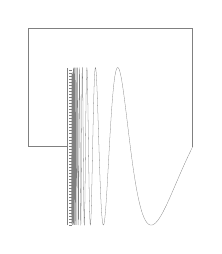
\begin{tikzpicture}[x=5cm]
\draw[gray,domain=0.01:1/pi,samples=2500,ultra thin]plot(\x,{sin(deg(1/\x))});
\draw[gray,thin](0,-1)--(0,1);
\draw[gray,ultra thin,densely dotted](0.003,-1)--(0.003,1)(0.006,-1)--(0.006,1)(0.009,-1)--(0.009,1);
\draw[gray,thin](0,0)--(-0.1,0)--(-0.1,1.5)--(1/pi,1.5)--(1/pi,-0.01);
\end{tikzpicture}

\noindent more formally, it is the quotient space $C \sqcup [0,1] \to W$ where 
we identify $0$ and $1$ with the appropriate points on $C$
} from the `free endpoint' of 
the oscillating path component to the other path component on the $y$-axis. Then $W$ is 
path connected, but still has all homotopy groups trivial. Thus the map $W\to \pt$ is a 
weak homotopy equivalence, but there is no contraction of $W$ as this would ultimately 
give rise to a path contained in the topologist's sine curve from one path component to 
the other.

\end{example}

Another class of examples illustrates why making a general assumption that our spaces are slpc is harmless from the point of view of homotopy theory.

\begin{definition}
For any space $X$, define the quotient topology on $[\pt,X]$ coming from the map $X\to [\pt,X]$. We can also consider the discrete space $\disc[\pt,X]$, which comes with a bijective map $\disc[\pt,X] \to [\pt,X]$. Define the space $\mathrm{slpc}(X)$ to be the pullback in the square
\[
	\xymatrix{
		\disc[\pt,X] \times_{[\pt,X]} X \ar[rr] \ar[d] && X \ar[d]\\
		\disc[\pt,X] \ar[rr] && [\pt,X]
	}
\]
\end{definition}

One way to think of this is that we put a new topology on the underlying set of $X$ so that it becomes the disjoint union of its path components.

\begin{lemma}
The assignment $X\mapsto \mathrm{slpc}(X)$ is the object component of a functor $\Top \to \Top$ landing inside the full subcategory of slpc spaces.
\end{lemma}

\begin{proof}
Exercise.
\end{proof}

By construction, there is a continuous, bijective map $\mathrm{slpc}(X) \to X$ that is the identity map on the underlying sets.

\begin{lemma}
The map $\mathrm{slpc}(X) \to X$ is a weak homotopy equivalence, and a is not a homotopy equivalence if $X$ is not already slpc.
\end{lemma}

Thus if we cannot tell apart spaces that are weakly homotopy equivalent, it is relatively harmless to work only with slpc spaces.

\section{Complexes}

Recall the Euler characteristic of a polyhedron $P$:
\[
	\chi(P) = \underbrace{\text{\#(vertices)}}_{0\text{-dim}} - \underbrace{\text{\#(edges)}}_{1\text{-dim}} + \underbrace{\text{\#(faces)}}_{2\text{-dim}}
\]
This definition doesn't require the polyhedron to be convex, simply-connected or even connected. It's not even restricted to surfaces, if we define
\[
	\chi(P) = \sum_{d=0}^{\dim P} (-1)^d \text{\#($d$-dim faces)}
\]
However, $\chi$ is not functorial in any way and so we cannot relate in any obvious way the Euler characteristics of different polyhedra. Ideally, we would have a functor from which we can then reconstruct the Euler characteristic. The key idea is to replace the vertex, edge, etc count by the dimension of some vector space. The vertx, edge, etc counts can be reconstructed from the vector space, but now we could in principle have an infinite-dimensional vector space, which would arise in the case that we have an \emph{infinite} polyhedron\marginnote{for instance a triangulation of an infinite-genus surface}


\begin{definition}
A \emph{complex} $A_\bullet$ (of vector spaces, abelian groups, $R$-modules) is a sequence 
\[
	\cdots \to A_{n-1} \xrightarrow{d_{n-1}} A_n \xrightarrow{d_n} A_{n+1} \to \cdots
\]
(of vector spaces, abelian groups, $R$-modules) such that $d_n\circ d_{n-1} = 
0$\marginnote{equivalently, $\im(d_{n-1}) \subseteq \ker(d_n)$} for all $n$
\end{definition}

\begin{example}
Any exact sequence, of abelian groups say, gives a complex.
\end{example}

As for exact sequences, we can have a section of the complex that consists of nontrivial 
groups, vector spaces etc and the rest of the complex can be trivial. In this case 
we can restrict attention to the nontrivial section.

\begin{example}
The following is a complex:
\[
	0\to \ZZ \xrightarrow{\times 4} \ZZ \xrightarrow{\mod{2}} \ZZ/2\ZZ \to 0
\]
Now we have an injective map on the left, and a surjective map on the right, but we only have that $4\ZZ < 2\ZZ$, not an equality of the kernel and the image.
\end{example}


\begin{example}
Let $A$ and $B$ be a pair of $n\times n$ real matrices such that $BA$ is the zero matrix, considered as linear maps. Then
\[
	0\to \RR^n \xrightarrow{A} \RR^n \xrightarrow{B} \RR^n \to 0
\]
is a complex. There is no way for this to be exact, because then $B$ would have to be surjective, hence invertible, and $A$ would have to be injective, hence invertible, but then we cannot have $BA=0$.
\end{example}

Here is an example which should be familiar from multivariable calculus. For $U\subset \RR^n$ an open subset, let $C^\infty(U)$ denote the vector space of smooth functions on $U$ and $C^\infty(U,\RR^3)$ be the vector space of vector fields on $U$.

\begin{example}
The various derivative operators $\nabla$ (gradient), $\nabla\times-$ (curl) and $\nabla\cdot -$ (divergence) give acomplex denoted $\Omega^\bullet(U)$:
\[
	C^\infty(U) \xrightarrow{\nabla} C^\infty(U,\RR^3) \xrightarrow{\nabla\times -} C^\infty(U,\RR^3) \xrightarrow{\nabla\cdot -} C^\infty(U) \to 0
\]
because the curl of a gradient is zero, and the divergence of a curl is zero.
\end{example}

\begin{definition}
A map of complexes\marginnote{sometimes called a \emph{chain map}} $A_\bullet \to 
B_\bullet$ consists of a sequence of maps $f_n\colon A_n \to B_n$ such that all the 
squares
\[
	\xymatrix{
		A_{n-1} \ar[r]^{d_{n-1}^A} \ar[d]_{f_{n-1}} & A_n \ar[d]^{f_n}\\
		B_{n-1} \ar[r]_{d_{n-1}^B} & B_n
	}
\]
The category of complexes of $R$-modules and chain maps is denoted $\Cplx_R$.
\end{definition}

\begin{example}
Given the matrices $A$ and $B$ from the previous example, there is map of complexes
\[
	\xymatrix{
		0 \ar[r] \ar@{=}[d] & 0 \ar[r] \ar[d] & \RR^n \ar[r]^A \ar[d] & \RR^n \ar[r]^B \ar[d] & \RR^n \ar[r] \ar[d] & 0 \ar@{=}[d]\\
		0 \ar[r] & \ker(A) \ar[r] & 0 \ar[r] & \RR^n/\im(A) \ar[r] & \RR^n \ar[r] & 0
	}
\]
\end{example}

\begin{example}
There is a map of complexes $\Omega^\bullet(\RR^3) \to \Omega^\bullet(U)$
\[
	\xymatrix{
	C^\infty(\RR^3) \ar[d] \ar[r]^{\nabla} & C^\infty(\RR^3,\RR^3) \ar[d] \ar[r]^{\nabla\times -} & C^\infty(\RR^3,\RR^3) \ar[d] \ar[r]^{\nabla\cdot -} & C^\infty(\RR^3) \ar[d] \ar[r] & 0 \ar[d] \\
	C^\infty(U) \ar[r]_{\nabla} & C^\infty(U,\RR^3) \ar[r]_{\nabla\times -} & C^\infty(U,\RR^3) \ar[r]_{\nabla\cdot -} & C^\infty(U)\ar[r] & 0
	}
\]
where the vertical maps restrict functions and vector fields.
\end{example}

Now the complex $\Omega^\bullet(\RR^3)$ is exact,\marginnote{by the Poincar\'e 
lemma, or more prosaically by standard multivariable calculus} because a vector field 
$\mathbf{v}$ on $\RR^3$ satisfies $\nabla\times \mathbf{v}=\mathbf{0}$ if and only if 
$\mathbf{v} = \nabla f$ for some function $f$, $\nabla\cdot \mathbf{v} = 0$ if and only 
if $\mathbf{v} = \nabla\times \mathbf{w}$ for some vector field $\mathbf{w}$, and any 
function $\RR^3\to \RR$ is the divergence of some vector field. Ultimately, this is 
because $\RR^3$ is contractible. But if we take $U = \RR^3\setminus\{0\}$, then there 
are vector fields $\mathbf{v}$ on $U$ with zero divergence that are not the curl of a 
vector field on $U$. This is because $\RR^3\setminus\{0\}$ is homotopy equivalent to 
$S^2$, and so the complex $\Omega^\bullet(\RR^3\setminus\{0\})$ can `see' the 
nontrivial topological structure also captured by $\pi_2(S^2) = \ZZ$. This is measured 
by the fact that the kernel of $\nabla\cdot -$ and the image of $\nabla\times -$ do not 
coincide.

Similarly, one can take $U = \RR^3 \setminus \ell$ where $\ell\subset \RR^3$ is a 
1-dimensional subspace.\marginnote{for instance $\ell=$ the $z$-axis} We have a homotopy 
equivalence between $\RR^3 \setminus \ell$ and $S^1$. And this is detected by the fact 
there are vector fields in $\RR^3 \setminus \ell$ whose curl vanishes but which are not 
the gradient of any function. Thus the kernel of $\nabla\times -$ and the image $\nabla$ 
are different. Ultimately, it is not the specific complex that captures the 
information of interest, because $\Omega^\bullet(\RR^n)$ is made up of enormous 
infinite-dimensional vector spaces, but $\RR^n$ itself is homotopically 
uninteresting.\marginnote{the keen-eyed will have noticed that the kernel of $\nabla$ 
consists of the constant functions, so is isomorphic to $\RR$. This one-dimensional 
vector space accounts for the fact $[\pt,\RR^3] = *$}

We will look at much smaller examples to properly warm up, to illustrate the type of 
algebra that will turn up.

\begin{definition}\label{eg:triangle_graph}
A \emph{simple directed graph} consists of a set $V$ of \emph{vertices}, a set $E$ of 
edges and two functions $d_0,d_1\colon E\to V$ such that $(d_0,d_1)\colon E \to V\times 
V$ is injective, and $\im (d_0,d_1) \cap \Delta(V) = \emptyset$\marginnote{$\Delta(V) = 
\{(v,v)\in V^2\}$ is the diagonal}
\end{definition}

Such a directed graph has no self-loops from a vertex to itself, and no more than one 
edge between any two vertices. The idea is that an edge $e$ points from $d_1(e)$ to 
$d_0(e)$.

\begin{example}\label{eg:triangle_graph}
Let $V = \{A,B,C\}$ and $E = \{a,b,c\}$, with\marginnote{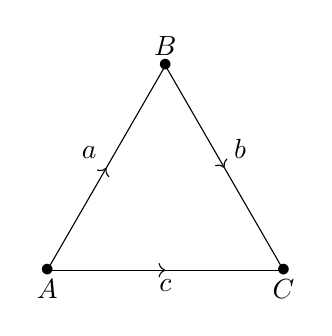
\begin{tikzpicture}
\draw[decoration={markings, mark=at position 0.5 with {\arrow{>}}},postaction={decorate}] 
(0,0) node {$\bullet$} --  node [auto] {$a$} (60:3);
\node[below] at (0,0) {$A$};

\draw[decoration={markings, mark=at position 0.5 with {\arrow{>}}},postaction={decorate}] 
(60:3) node {$\bullet$} -- node [auto] {$b$} (3,0); 
\node[above] at (60:3) {$B$};

\draw[decoration={markings, mark=at position 0.5 with {\arrow{>}}},postaction={decorate}] 
(0,0)  -- node [auto,swap] {$c$} (3,0) node {$\bullet$};
\node[below] at (3,0) {$C$};
\end{tikzpicture}}
\[
(d_1,d_0) \colon \begin{cases}
a & \mapsto (A,B)\\
b & \mapsto (B,C)\\
c & \mapsto (A,C)
\end{cases}
\]
This graph is denoted $\partial \Delta[2]$, for reasons that will become clearer below.
\end{example}

To define a complex from a directed simple graph, for any given set $S$ and ring $R$, let $R^S$ denote the $R$-module\marginnote{if $R=\ZZ$, this is the product of $|S|$-many copies of $\ZZ$, and if $R$ is a field, it's the vector space of functions on $S$} of functions $f\colon S\to R$. The following definition is made using $R=\ZZ$, but it works for any ring $R$ more generally.

\begin{definition}
Let $d_0,d_1\colon E\rightrightarrows V$ be a simple directed graph. Define the complex
\begin{align*}
0 \quad \to \quad \ZZ^V & \quad\xrightarrow{\delta} \qquad\ZZ^E  \qquad \to \quad 0\\
f \quad & \mapsto\  f\circ d_0 - f\circ d_1
\end{align*}
\end{definition}

Here\lecturenum{20} are a bunch of concrete examples

\begin{example}
Consider the trivial graph with one vertex and no edges. The complex is $0\to \ZZ \xrightarrow{\delta} 0 \to 0$, and clearly $\ker(\delta)=\ZZ$ and $\coker(\delta) = 0$.
\end{example}

\begin{example}
The complex that arises from $\partial\Delta[2]$ in Example~\ref{eg:triangle_graph} is 
$0\to\ZZ^3\xrightarrow{\delta} \ZZ^3 \to 0$. We can identify a generating set of 
$\ZZ^3 = \ZZ^V$, namely $\underline{X}\colon\{A,B,C\}\to \ZZ$ for $X\in \{A,B,C\}$ with
\[
	\underline{A}(v) = \begin{cases}
				1 & v=A\\
				0 & \text{else}
	\end{cases}
\]
and similarly for $\underline{B}$ and $\underline{C}$. We can calculate
\begin{align*}
	\delta(\underline{A})(e) & = \underline{A}(d_0(e)) - \underline{A}(d_1(e))\\
							& =\begin{cases}
							-1 & e=a\\
							0 & e=b\\
							-1& e=c
							\end{cases}
\end{align*}
We can see this from the graph itself, in that the vertex $A$ is the source of the edges $a$ and $c$, and isn't incident with the edge $b$. To contrast, $\delta(\underline{B})(a) = 1$, as $B$ is the target of the edge $a$. We can then write down the matrix $D$ representing $\delta$, namely
\[
	D = \begin{pmatrix}
		-1 & 0 & -1\\
		1 & -1 & 0\\
		0 & 1 & 1
	\end{pmatrix}
\]
We can calculate that $\ker(D)$ is torsion-free and generated by $\underline{A} + \underline{B} - \underline{C}$, hence is isomorphic to $\mathbb{Z}$. Similarly, the image of $D$ is generated by $\underline{A} - \underline{B}$ and $\underline{B} - \underline{C}$, and, incidentally, $\ZZ^E$ is generated by these two functions together with $\underline{B}$, so that the $\coker(D) \simeq \ZZ$. As a final remark, note that the Euler characteristic $\chi=0$.
\end{example}

\begin{rem}\label{remark:finite_complexes_basis}
For any \emph{finite} graph (and later, more general finite combinatorial objects), we can take the vertices and the edges to represent generating sets for $\ZZ^V$ and $\ZZ^E$. But for infinite graphs, this is not the case, and we'd have to be more careful.
\end{rem}

\begin{example}\label{eg:triangle_graph}
Consider\marginnote{%
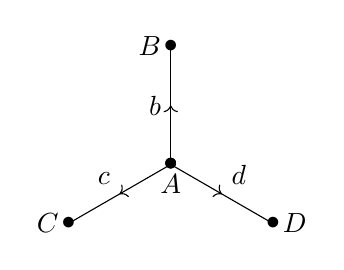
\begin{tikzpicture}
\draw[decoration={markings, mark=at position 0.5 with {\arrow{>}}},postaction={decorate}] 
(0,0) node {$\bullet$} --  node [auto] {$d$} (-30:1.5) node{$\bullet$};
\node[below] at (0,0) {$A$};
\node[right] at (-30:1.5) {$D$};

\draw[decoration={markings, mark=at position 0.5 with {\arrow{>}}},postaction={decorate}] 
(0,0) node {$\bullet$} --  node [auto,swap] {$c$} (-150:1.5) node {$\bullet$};
\node[left] at (-150:1.5) {$C$};

\draw[decoration={markings, mark=at position 0.5 with {\arrow{>}}},postaction={decorate}] 
(0,0) node {$\bullet$} --  node [auto] {$b$} (0,1.5) node{$\bullet$};
\node[left] at (0,1.5) {$B$};
\end{tikzpicture}} 
the graph with four vertices $\{A,B,C,D\}$ and three edges $\{b,c,d\}$ as at right. The complex that arises is $0\ZZ^4\xrightarrow{\delta} \ZZ^3 \to 0$, where $\delta$ is represented by
\[
	D = \begin{pmatrix}
		-1 & 1 & 0 & 0\\
		-1 & 0 & 1 & 0\\
		-1 & 0 & 0 & 1
	\end{pmatrix}
\]
with respect to the generating set as in Remark~\ref{remark:finite_complexes_basis}. The 
image is all of $\ZZ^3$, hence the cokernel is trivial, and the kernel is $\ZZ$. For 
this example we have $\chi = 1$.
\end{example}

We don't have to use connected graphs!

\begin{example}
Consider\marginnote{%
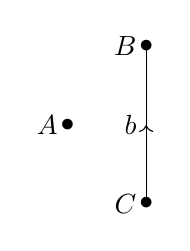
\begin{tikzpicture}
\node at (-1,1) {$\bullet$};
\node[left] at (-1,1) {$A$};
\draw[decoration={markings, mark=at position 0.5 with {\arrow{>}}},postaction={decorate}] 
(0,0) node {$\bullet$} --  node [auto] {$b$} (0,2) node{$\bullet$};
\node[left] at (0,2) {$B$};
\node[left] at (0,0) {$C$};
\end{tikzpicture}}
the graph with vertex set $\{A,B,C\}$, edge set $\{b\}$ such that $d_0(b)=B$, 
 $d_1(b)=C$. The complex is $0\to \ZZ^3 \xrightarrow{\delta} \ZZ \to 0$, with 
 $\delta$ onto, hence $\coker(\delta)=0$. The kernel of $\delta$ is $\ZZ^2$, and the 
 Euler characteristic is $2$.

\end{example}

\begin{ex}
\begin{enumerate}
\item Given any two simple directed graphs $G_1$, $G_2$, we can define the disjoint 
union $G_1 \sqcup G_2$ by taking the disjoint union of their edges and vertices and 
taking the induced functions $d_0, d_1$. Show $\ker \delta_{G_1\sqcup G_2} \simeq \ker 
\delta_{G_1} \oplus \ker \delta_{G_2}$.

\item For any directed graph $G$ with underlying shape a polyhedron, show that the 
kernel and cokernel of the associated map $\delta_G$ both isomorphic to $\ZZ$.
\end{enumerate}
\end{ex}

The first of these two exercises prove that $\dim\ker\delta$ counts the number of 
connected components, and the second strongly suggest that $\dim\coker\delta$ counts the 
number of loops.

\begin{ex}
Calculate the kernel and cokernel of a connected simple directed graph with two cycles.
\end{ex}

\begin{rem}
It is entirely possible to work not just with simple directed graphs, but general directed 
graphs, since the definition of the complex associated to a graph as above does not use the 
injectivity of $(d_0,d_1)$ or disjointness from the diagonal. Thus\marginnote{
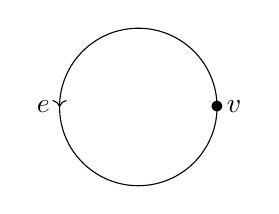
\begin{tikzpicture}
\draw[decoration={markings, mark=at position 0.5 with {\arrow{>}}},postaction={decorate}] (0,0) circle [radius = 1];
\node at (1,0) {$\bullet$};
\node[right] at (1,0) {$v$};
\node[left] at (-1,0) {$e$};
\end{tikzpicture}} 
we can consider a directed
graph with one vertex and one edge---a combinatorial model of the circle---and get the complex
$0\to \ZZ \xrightarrow{\delta=0} \ZZ\to 0$, where now $\ker\delta=\ZZ$ and $\coker\delta=\ZZ$,
as in Example~\ref{eg:triangle_graph}.
\end{rem}


However, as much fun as this is, we really need to think about more than just 
1-dimensional objects. This leads to the question of what the two-dimensional version of 
a directed graph is. One option is the following: take sets of vertices, edges and 
triangular faces, and specify how they fit together, by means of functions analogous to 
$d_0$ and $d_1$ from before.\marginnote[-1cm]{I would call this (2-skeletal) semisimplicial 
set, but Mike Hopkins called such a thing a \emph{combinatorial $\Delta$-complex}}


\begin{example}\label{eg:triangle_Delta_complex}
Consider\marginnote{
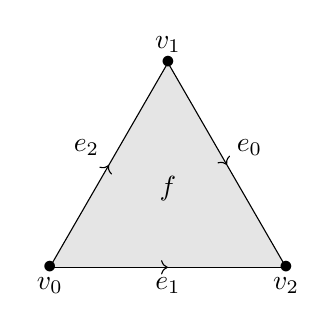
\begin{tikzpicture}
\path [fill=gray!20!white] (0,0) -- (60:3) -- (3,0) -- cycle;
\node at (1.5,1) {$f$};

\draw[decoration={markings, mark=at position 0.5 with {\arrow{>}}},postaction={decorate}] 
(0,0) node {$\bullet$} --  node [auto] {$e_2$} (60:3);
\node[below] at (0,0) {$v_0$};

\draw[decoration={markings, mark=at position 0.5 with {\arrow{>}}},postaction={decorate}] 
(60:3) node {$\bullet$} -- node [auto] {$e_0$} (3,0); 
\node[above] at (60:3) {$v_1$};

\draw[decoration={markings, mark=at position 0.5 with {\arrow{>}}},postaction={decorate}] 
(0,0)  -- node [auto,swap] {$e_1$} (3,0) node {$\bullet$};
\node[below] at (3,0) {$v_2$};
\end{tikzpicture}
}
 just a single, filled triangle. Let the vertices be called $v_0$, $v_1$ and 
$v_2$. There are edges $e_0$, $e_1$ and $e_2$, and one face, $f$.
\end{example}

Note that in this triangle, $d_0(e_2)=d_1(e_0)$ and so on, where $e_i$ is the edge opposite 
the vertex $v_i$. The combinatorics of how the edges and vertices fit together are captured
in the following definition. 


\begin{definition}

A \emph{combinatorial surface} $X_\bullet$ consists of sets of vertices, 
edges and faces, denoted\marginnote{so that $X_i$ is 
the set of $i$-dimensional `faces'; the functions $d_i^n$ are called \emph{face maps}} $X_0$, $X_1$ and $X_2$ respectively together with 
functions $d_i^n\colon X_n \to X_{n-1}$ for all $0\leq i \leq n$, $0<n\leq 2$ such 
that\marginnote[4ex]{the easiest way to remember 
these identities is to draw the triangle in Example~\ref{eg:triangle_Delta_complex}}
\begin{align}\label{eq:simpl_ids_surf}
d_0^1\circ d_2^2 & = d_1^1\circ d_0^2, \nonumber\\
d_0^1\circ d_1^2 & = d_0^1\circ d_0^2,\\
d_1^1\circ d_2^2 & = d_1^1\circ d_1^2. \nonumber
\end{align}
When the context is clear, we can usually the superscripts, as the dimension can be inferred
from the data. The \emph{1-skeleton} of $X_\bullet$ is the underlying directed graph 
gotten by forgetting $X_2$.
\end{definition}

Now note that `surface' here is really a stand-in for `at most 2-dimensional'. There is nothing
in the definition that requires that $X_2\neq \emptyset$. And,\marginnote{%
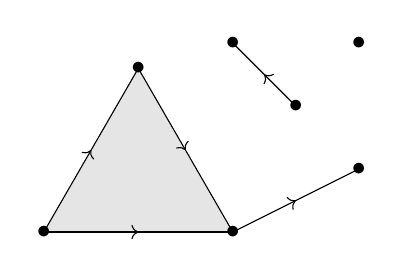
\begin{tikzpicture}[scale=0.8]
\path [fill=gray!20!white] (0,0) -- (60:3) -- (3,0) -- cycle;
\draw[decoration={markings, mark=at position 0.5 with {\arrow{>}}},postaction={decorate}] 
(0,0) node {$\bullet$} --   (60:3);

\draw[decoration={markings, mark=at position 0.5 with {\arrow{>}}},postaction={decorate}] 
(60:3) node {$\bullet$} -- (3,0); 

\draw[decoration={markings, mark=at position 0.5 with {\arrow{>}}},postaction={decorate}] 
(0,0)  -- (3,0) node {$\bullet$};

\draw[decoration={markings, mark=at position 0.5 with {\arrow{>}}},postaction={decorate}] 
(3,0) -- (5,1)  node {$\bullet$};
\draw[decoration={markings, mark=at position 0.5 with {\arrow{>}}},postaction={decorate}] 
(4,2) -- (3,3)  node {$\bullet$};
\node at (4,2) {$\bullet$};
\node at (5,3) {$\bullet$};
\end{tikzpicture}
}
moreover, it is possible 
to have 0- or 1-dimensional `components' in a surface, much as a graph is generically 1-dimensional,
but can have isolated vertices, or even consist purely of vertices and no edges. In this way, 
a combinatorial surface could be so degenerate it has no triangles and no edges, but if 
there is at least one triangle, then there must be at least one edge (and at least one vertex).


\begin{example}
The triangle from Example~\ref{eg:triangle_Delta_complex} is denoted $\Delta[2]$, and has 
$\Delta[2]_0 = \{v_0,v_1,v_2\}$, $\Delta[2]_1 = \{e_0,e_1,e_2\}$ and $\Delta[2]_2 = \{f\}$, 
$d^2_i(f) = e_i$ and $d^1_0,d^1_1\colon \Delta[2]_1\to \Delta[2]_0$ 
as in Example~\ref{eg:triangle_graph}, up to relabelling. The 1-skeleton of $\Delta[2]$ 
is the directed graph $\partial\Delta[2]$.
\end{example}

As noted above, we do not need to restrict to the case where the 1-skeleton is a simple directed
graph, and so it can be any directed graph.

\begin{example}\label{eg:combinatorial_torus}
We can provide a combinatorial model of a torus, $T_\bullet$, by taking $T_0 = \{v\}$, 
$T_1 = \{e_1,e_2,e_3\}$ and $T_2 = \{f_1,f_2\}$ fitting together as

\begin{center}
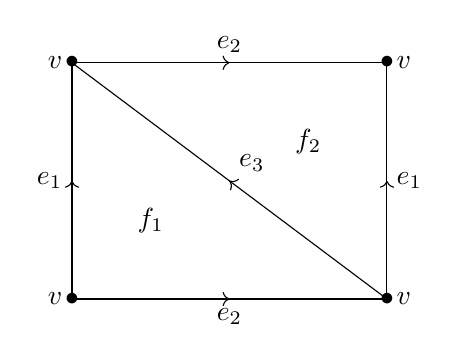
\begin{tikzpicture}
\draw[decoration={markings, mark=at position 0.5 with {\arrow{>}}},postaction={decorate}] 
(0,0) node {$\bullet$} --  node [auto] {$e_1$} (0,3);
\node[left] at (0,0) {$v$};

\draw[decoration={markings, mark=at position 0.5 with {\arrow{>}}},postaction={decorate}] 
(0,3) node {$\bullet$} --  node [auto] {$e_2$} (4,3);
\node[left] at (0,3) {$v$};

\draw[decoration={markings, mark=at position 0.5 with {\arrow{>}}},postaction={decorate}] 
(4,0) node {$\bullet$} --  node [auto,swap] {$e_1$} (4,3) node {$\bullet$};
\node[right] at (4,3) {$v$};

\draw[decoration={markings, mark=at position 0.5 with {\arrow{>}}},postaction={decorate}] 
(0,0) --  node [auto,swap] {$e_2$} (4,0);
\node[right] at (4,0) {$v$};

\draw[decoration={markings, mark=at position 0.5 with {\arrow{>}}},postaction={decorate}] 
(4,0) --  node [auto,swap] {$e_3$} (0,3);

\node at (1,1) {$f_1$};
\node at (3,2) {$f_2$};
\end{tikzpicture}
\end{center}
Thus, $d^2_0(f_1)=e_3$, $d^2_1(f_1)=e_1$ and $d^2_2(f_1) = e_2$; $d^2_0(f_2) = e_2$, 
$d^2_1(f_2) = e_1$, $d^2_2(f_2) = e_3$, and $d^1_0(e_i) = v = d^1_1(e_i)$ for $e=1,2,3$.
\end{example}

Given a combinatorial surface $X_\bullet$, we can define a sequence $C^\bullet(X_\bullet)$ 
of abelian groups in a similar way as 
for a directed graph:\marginnote{here taking the ring $R=\ZZ$ for simplicty, the general 
definition works the same}
\[
0\to \ZZ^{X_0} \xrightarrow{\delta_0} \ZZ^{X_1} \xrightarrow{\delta_1} \ZZ^{X_2} \to 0
\]
where $\delta_0$ is defined the same way as for a directed graph: $\delta_0(g) = gd^1_0 - 
gd^1_1\colon X_1 \to \ZZ$ for $g\in \ZZ^{X_0}$ and $\delta_1(g') = g'd^2_0 - g'd^2_1 + g'd^2_2 = 
\sum_{i=0}^2g'd_i \colon X_2 \to \ZZ$ for $g'\in \ZZ^{X_1}$. We will see below that this is 
indeed a complex.

\begin{rem}\label{rem:basis_finite_complex}
If the combinatorial surface has $X_i$ finite for $i=0,1,2$, then we can 
take as basis for $\ZZ^{X_i}$ the set $X_i$, where we identify an element $x\in X_i$ with 
the function $X_i\to \ZZ$ that is equal to $1$ when evaluated on $x$, and otherwise is $0$.
It was remarked in class that some sources consider functions that are only nonzero on 
finitely many elements of $X_n$, but this is not what we are doing here, and even the maps
$\delta_i$ cease to become well-defined, as infinitely many edges might share a vertex, for 
example. For infinite complexes we need to rely on more abstract means to describe the maps $\delta_i$,
 if we want them explicity in terms of a basis. 
\end{rem}

\begin{example}
Given the combinatorial surface $T_\bullet$ from Example~\ref{eg:combinatorial_torus}, the 
resulting sequence is 
\[
	0 \to \ZZ \xrightarrow{\delta_0} \ZZ^3 \xrightarrow{\delta_1} \ZZ^2 \to 0
\]
where $\delta_0(g)(e) = g(d_0(e)) - g(d^2_1(e)) = g(v) - g(v) = 0$ for any edge $e\in X_1$, 
and so is the zero map. If we take the basis as in the previous
Remark, the map $\delta_1$ is represented by the matrix
\[
	\begin{pmatrix}
	-1&1&1 \\
	-1&1&1
	\end{pmatrix}
\] 
and the composite $\delta_1\delta_0$ is clearly the zero map, so this is a complex.
\end{example}

\begin{lemma}
For any combinatorial surface $X_\bullet$, the sequence $C^\bullet(X_\bullet)$ is a complex.
\end{lemma}

\begin{proof}
We need to prove that for any $g\colon X_0\to \ZZ$, and any $x\in X_2$, we have
$\delta_1(\delta_0(g))(x) = 0$.
\begin{align*}
\delta_1(\delta_0(g))(x) & = \delta_1(g d^2_0 - gd^2_1)(x)\\
			 & = \delta_1(gd^2_0)(x) - \delta_1(gd^2_1)(x)\\
			 & = gd^1_0d^2_0(x) - gd^1_0d^2_1(x) + gd^1_0d^2_2(x) \\
			 & - (gd^1_1d^2_2(x) - gd^1_1d^2_1(x) + gd^1_1d^2_2(x))\\
			 & = 0 
\end{align*}
where in the last step we use the equations (\ref{eq:simpl_ids_surf}).
\end{proof}

The combinatorial torus above has Euler characteristic $\chi=1 - 3 + 2 = 0$, but if we look
at the failure of it to be exact, we get $\ker\delta_0 \simeq \ZZ$, $\coker\delta_1 \simeq \ZZ$, and 
$\ker\delta_1/\im\delta_0 \simeq \ZZ^2$.

\begin{rem}
We could have taken an arbitrary (commutative, unital) ring $R$ instead of $\ZZ$ in the 
above example, and the resulting $\ker\delta_0$ etc would be $R$-modules. For $R=\ZZ$ these are
$\ZZ$-modules, hence abelian groups, but for example taking $R=\ZZ/2$ we get abelian groups, 
but they have more structure as $\ZZ/2$-modules.
\end{rem}


\begin{ex}
Calculate\marginnote{Hint: label the vertices $0,1,2,3$, order the edges from from lower to 
higher labels, and then define the maps $d_0,d_1,d_2$ for faces using $\Delta[2]$ as a model} 
the complex of abelian groups arising from a tetrahedron considered as a combinatorial
surface, and the groups $\ker\delta_0$, $\ker\delta_1/\ker\delta_0$.
\end{ex}

\begin{ex}
Consider\marginnote{%
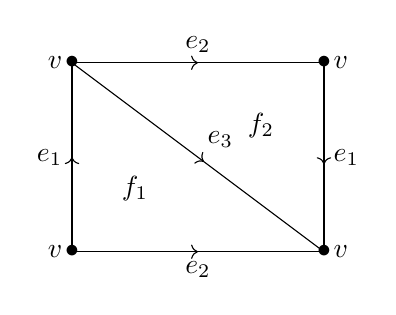
\begin{tikzpicture}[scale=0.8]
\draw[decoration={markings, mark=at position 0.5 with {\arrow{>}}},postaction={decorate}] 
(0,0) node {$\bullet$} --  node [auto] {$e_1$} (0,3);
\node[left] at (0,0) {$v$};

\draw[decoration={markings, mark=at position 0.5 with {\arrow{>}}},postaction={decorate}] 
(0,3) node {$\bullet$} --  node [auto] {$e_2$} (4,3);
\node[left] at (0,3) {$v$};

\draw[decoration={markings, mark=at position 0.5 with {\arrow{<}}},postaction={decorate}] 
(4,0) node {$\bullet$} --  node [auto,swap] {$e_1$} (4,3) node {$\bullet$};
\node[right] at (4,3) {$v$};

\draw[decoration={markings, mark=at position 0.5 with {\arrow{>}}},postaction={decorate}] 
(0,0) --  node [auto,swap] {$e_2$} (4,0);
\node[right] at (4,0) {$v$};

\draw[decoration={markings, mark=at position 0.5 with {\arrow{<}}},postaction={decorate}] 
(4,0) --  node [auto,swap] {$e_3$} (0,3);

\node at (1,1) {$f_1$};
\node at (3,2) {$f_2$};

\end{tikzpicture}
}
a combinatorial model of the Klein bottle $K_\bullet$, with two triangles, 
three edges and one vertex, as in the sketch at right, where $d_0(f_1) = e_3$, 
$d_1(f_1) = e_2$ and $d_2(f_1) = e_1$, and $d_0(f_2) = e_1$, $d_1(f_2) = e_2$ and $d_2(f_2) = e_2$.
And, as for the combinatorial torus, $d_0(e_i) = x = d_1(e_i)$ for $i=1,2,3$.
(The triangles are considered to be filled, despite the lack of shading.)
\end{ex}


\begin{definition}
Given a complex $A_\bullet$ of $R$-modules, and an integer $n$, the $n^{th}$ cohomology 
$H^n(A_\bullet)$ is the $R$-module
\[
\frac{\ker A_n \xrightarrow{d_n} A_{n+1}}{\im A_{n-1} \xrightarrow{d_{n-1}} A_n}
\]
\end{definition}

\begin{lemma}
For all integers $n$, $H^n \colon \Cplx_R \to R\Mod$ is a functor.
\end{lemma}

\begin{proof}
Exercise.
\end{proof}

Here is the big idea: spaces and their homotopy groups are hard, so to study one, turn 
it into a complex, then look at the cohomology groups instead. And, we want this 
to be a functor. We have seen so far that
\[
\pi_i(S^2,*) = \begin{cases}
* & i=0\text{ connected}\\
0 & i=1\text{ by Seifert--van~Kampen}\\
\ZZ & i=2\text{ without proof!}\\
\ZZ & i=3\text{ also without proof!}\\
\vdots &
\end{cases}
\]
However, we can calculate the cohomology groups of the combinatorial surface $T_\bullet$ using
just linear algebra, and these seem to capture at least some of this information, with much less
work. There are some caveats, in that we haven't actually constructed a functor assigning to
a combinatorial surface its cohomology groups, and, worse, there's no guarantee that a 
combinatorial tetrahedron (as opposed to an actual space!) really captures the topology of $S^2$.
But it should be suggestive as to a different approach.

\begin{rem}
This\lecturenum{21} lecture started with a long recap of the previous lecture, and I have
gone back and incorporated some of this material just above, in the section labelled 
lecture 20.
\end{rem}

Note that given a combinatorial surface $X_\bullet$ and a ring $R$ we have cohomology groups
\begin{align*}
H^0(X_\bullet,R) & := \ker\delta_0\\
H^1(X_\bullet,R) & := \frac{\ker\delta_1}{\im\delta_0}\\
H^2(X_\bullet,R) & := \frac{R^{X_2}}{\im\delta_1} = \coker\delta_1
\end{align*}
arising from the complex $0\to R^{X_0} \to R^{X_1} \to R^{X_2} \to 0$. We technically have 
$H^n(X_\bullet,R)$ for all integers $n$, but these are all the zero module. 
If $X_2=\emptyset$, then $R^{X_2} = R^\emptyset = \{0\}$, and so $H^2(X_\bullet,R) = \{0\}$.

We calculated the cohomology with $R=\ZZ$ for the combinatorial torus $T_\bullet$ above to be
\[
	H^n(T_\bullet,\ZZ) = \begin{cases}
				\ZZ & n=0\\
				\ZZ^2 & n=1\\
				\ZZ & n=2
			     \end{cases}
\]
But, the combinatorial surface $T_\bullet$ is very definitely not the topological space 
$S^1\times S^1$! So we need a way to relate actual topological spaces to this combinatorial
data. If we go back to the directed graph $\partial\Delta[2]$, it looks like it should be a
circle (topologically, at least). We could make an actual circle by taking the disjoint union
of three intervals $[0,1]$ and forming a quotient space so the endpoints are appropriately
identified. This idea is called geometric realisation. The following does not work, but gives
an idea of how the real version might go.

\begin{constr}
(Attempt 1) Given a directed graph $X_1 \rightrightarrows X_0$ We could try to take the 
quotient of $\bigsqcup_{X_1} I$, where we identify the endpoints of the different copies of 
$I$ according to the incidence of edges in the graph. But, this information is recorded 
in which edges map to the same vertex under the maps $d_0,d_1$, so we should involve these
functions somehow. A bigger problem is what to do with isolated vertices! They certainly are
not given by gluing intervals in any sense. So we need to use $X_0$ as well.
\end{constr}

\begin{construction}

(Attempt 2) We could instead take the discrete space on the set of vertices of a 
directed graph, and then attach the intervals to them. In this sense, any isolated 
vertices turn up in the construction, and any edge only needs to know what vertices it 
is incident with, which is indeed the case by the definition of directed graph. To get 
this working we need some topological ingredients. Consider\marginnote{these are in one 
sense `dual' to the combinatorial endpoint functions $d_0,d_1$} the functions 
$\partial_0,\partial_1\colon \pt\to I$ with $\partial_0(\pt) = 1$ and 
$\partial_1(\pt)=0$. Then the geometric realisation of a directed graph $X_1 
\rightrightarrows X_0$ should be $(\bigsqcup_{X_0}\pt \sqcup \bigsqcup_{X_1} I)/\!\sim$ 
where the equivalence relation identifies $(e,\partial_i(v))\sim(d_i(e),v)$. That is, 
the $i$-endpoint of the interval indexed by the element $e\in X_1$ should be identified 
with the point indexed by the vertex $v$. 
\end{construction}

This rough construction will soon be superceded by a more formal and systematic definition, 
but it should capture the idea.

\begin{example}\label{eg:join_interval_geom_real}
Consider the directed graph given by three vertices $\{v_1,v_2,v_3\}$ and two edges 
$\{e_1,e_2\}$ with $d_1(e_1) = v_1$, $d_0(e_1) = v_2 = d_1(e_2)$ and $d_0(e_2) = v_3$. Its 
geometric realisation is homeomorphic to $(\{v_1,v_2,v_3\} \sqcup [0,1] \sqcup [2,3])/\!\sim$
where $0\sim v_1$, $1\sim v_2 \sim 2$ and $3\sim v_3$. Thus it is homeomorphic to 
$([0,1]\sqcup [2,3])/(1\sim 2) \simeq [0,2] \simeq [0,1]$.
\end{example}

Now, how do so something similar for combinatorial surfaces? Now we must make some definitions
that will generalise more easily down the track, that are less ad hoc.

\begin{definition}
The \emph{standard $n$-simplex} is the subspace of $\RR^{n+1}$ given by
\[
	\Delta^n := \{(v_0,v_1,\ldots,v_n) \in \RR^{n+1} \mid \forall\, 0\leq i\leq n, v_i\geq 0
			\text{ and } v_0+\cdots+v_n = 1\}
\]
\end{definition}

\begin{example}
So\marginnote{
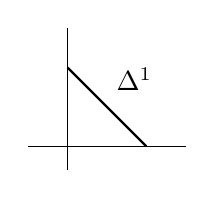
\begin{tikzpicture}
\draw (0,1.5) -- (0,-0.3) (-0.5,0)-- (1.5,0);
\draw[thick] (0,1) -- (1,0);
\node at (45:1.2) {$\Delta^1$};
\end{tikzpicture}\quad
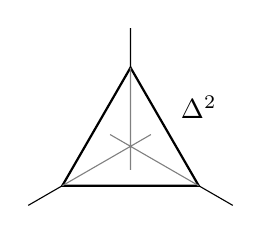
\begin{tikzpicture}
\draw[thick] (90:1) -- (-30:1) -- (-150:1) -- cycle;
\draw[gray] (-150:1) -- (30:0.3) (90:1)--(-90:0.3) (-30:1)--(150:0.3);
\draw (-150:1) -- (-150:1.5) (90:1) -- (90:1.5) (-30:1) -- (-30:1.5);
\node at (30:1) {$\Delta^2$};
\end{tikzpicture}
}  the standard $0$-simplex is a single point, namely $v_0=1\in \RR$, the standard $1$-simplex
is the interval $\Delta^1 = \{(v_0,v_1\in \RR^2\mid v_0,v_1 \geq0,\ v_0+v_1 = 1\}$, and the 
standard $2$-simplex is the portion of the hyperplane $v_0+v_1+v_2 = 1$ with the positive
octant in $\RR^3$. 
\end{example}

There are inclusion maps between the standard $n$-simplices, namely $\partial_i\colon \Delta^n \to \Delta^{n+1}$
defined to be $\partial_i(v_0,\ldots,v_n) = (v_0,\ldots,v_{i-1},0,v_i,\ldots,v_n)$, where
$0\leq i \leq n+1$.

\begin{example}
We have the two maps $\partial_0,\partial_1\colon \Delta^0 \to \Delta^1$ from before, $\partial_0(v_0) = (0,v_0) = (0,1)$ 
and $\partial_1(v_0) = (v_0,0) = (1,0)$. And now, imporantly, maps $\partial_i\colon \Delta^1\to \Delta^2$, $i=0,1,2$ with
\[
\partial_i(v_0,v_1) =\begin{cases}
(0,v_0,v_1) & i=0\\
(v_0,0,v_1) & i=1\\
(v_0,v_1,0) & i=2
\end{cases}
\]
\end{example}

\begin{definition}
The \emph{geometric realisation} of a combinatorial surface $X_\bullet$ is the quotient space
\[
|X_\bullet| := \left(\bigsqcup_{n=0}^2 \disc(X_n) \times \Delta^n\right)_{\big/\!\sim}
\]
where the equivalence relation is generated by 
$(d_i(x),\mathbf{v}) \sim (x,\partial_i(\mathbf{v}))$.
\end{definition}

For\marginnote{And, more degenerately, $|\Delta[1]| = \Delta^1$ and $|\Delta[0]|=\Delta^0$} 
instance, the geometric realisation of $\Delta[2]$ is 
\[
\Big((\Delta^0 \sqcup \Delta^0 \sqcup \Delta^0) \sqcup (\Delta^1 \sqcup 
\Delta^1 \sqcup\Delta^1) \sqcup\Delta^2\Big)/\!\sim\ \simeq\ (\partial\Delta^2 \sqcup\Delta^2)/\!\sim\ \simeq\ \Delta^2
\]

Let us, for the sake of the following definition, be generous with the definition of `surface';
it should include at least all topological manifolds of dimension 2 or lower, and even of mixed
dimension (eg the disjoint union of a circle and a torus). The important thing is that a
surface here is a topological space, not a combinatorial object.

\begin{definition}
A \emph{triangulation} of a surface $\Sigma$ is a combinatorial surface $X_\bullet$ equipped
with\marginnote{we will usually leave the homeomorphism implicit in what follows} 
a homeomorphism $\Sigma \simeq |X_\bullet|$.
\end{definition}

\begin{example}
\begin{enumerate}
\item $\Delta^2$ is triangulated by $\Delta[2]$.
\item More generally, $|X_\bullet|$ is triangulated by $X_\bullet$.
\item $S^2$ is triangulated by $\partial\Delta[3]$.
\item $S^1$ is triangulated by $\partial\Delta[2]$, but also by any directed graph in the shape
of a polygon, or even the directed graph with one vertex and one edge.
\item $S^1\times S^1$ is triangulated by the combinatorial torus $T_\bullet$.
\end{enumerate}
\end{example}



Ultimately,\lecturenum{22} of course, we want some kind of functorial behaviour, so we need
maps between combinatorial surfaces. The idea is that vertices get mapped to vertices, edges
to edges, and triangles to triangles, in a compatible way.

\begin{definition}
Given combinatorial surfaces $X_\bullet$ and $Y_\bullet$, a map $f\colon X_\bullet\to Y_\bullet$ 
is a triple of functions $f_n\colon X_n\to Y_n$, $n=0,1,2$ such that $d_if_n = f_{n-1}d_i$ for $0<n\leq 2$, $0\leq i \leq n$.
\end{definition}

Such maps are very rigid, in the sense that there are `obvious' functions between the intended
geometric objects that don't come from a map between given combinatorial surfaces. This
definition also includes map between directed graphs, if we take the set of triangles
to be empty, and maps from a directed graph to a non-degenerate combinatorial surface.

\begin{example}
Given a combinatorial surface $X_\bullet$, and its 1-skeleton $\sk_1 X_\bullet$, there is a morphism
$\sk_1X_\bullet\to X_\bullet$ that is the identity on $X_0$ and $X_1$, and the only possible 
function $(\sk_1X_\bullet)_2 = \emptyset \to X_2$. 
\end{example}

\begin{example}
We can include a single triangle into a combinatorial surface $X_\bullet$, via 
$\Delta[2] \to X_\bullet$. For instance, $\Delta[2] \to \partial\Delta[3]$.
\end{example}

\begin{example}
If $L_\bullet$ is the directed graph with one vertex and one edge, and $P_\bullet$ is any
polygonal\marginnote{a polygonal directed graph is a finite directed graph with the same number
of vertices and edges, the vertices are cyclicly ordered, and there is an edge between adjacent vertices, in either direction} 
directed graph (for instance $\partial\Delta[2]$), then there is a map
$P_\bullet \to L_\bullet$, sending all vertices to the single vertex of $L_\bullet$, and
all edges to the singe edge. We can even triangulate $\RR$ by taking an infinite directed 
graph $R_\bullet$  with vertices indexed by $\ZZ$ and an edge from $k$ to $k+1$, and then
define a map $R_\bullet \to L_\bullet$ in a similar way.
\end{example}

\begin{example}\label{eg:infinite_cylinder}
For a similar but nondegenerate example, we can define an infinite combinatorial surface that
models an infinite cylinder, with set of faces $\{f_{1i},f_{2i}\mid i \in \ZZ\}$, set of 
edges $\{e_{1i},e_{2i},e_{3i}\mid i\in \ZZ\}$ and set of vertices $\{v_i\mid i\in \ZZ\}$ as
in the following picture,

\begin{center}
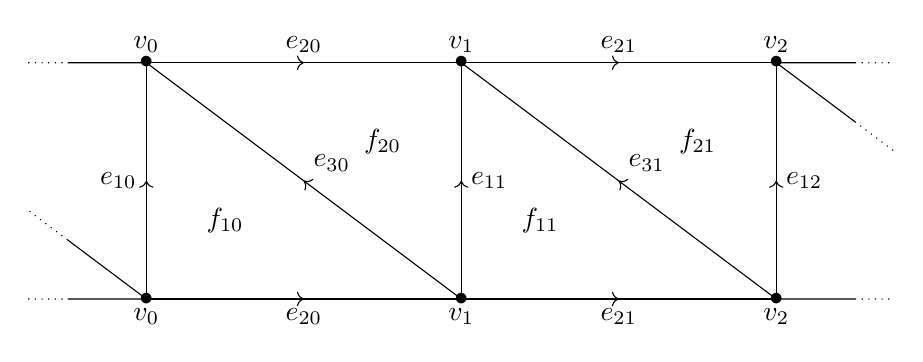
\begin{tikzpicture}

\draw (-1,0)--(0,0)--(-1,0.75)  (-1,3) -- (0,3);
\draw[dotted] (-1.5,0) -- (-1,0) (-1.5,3) -- (-1,3) (-1,0.75)--(-1.5,1.125);

\draw[decoration={markings, mark=at position 0.5 with {\arrow{>}}},postaction={decorate}] 
(0,0) node {$\bullet$} --  node [auto] {$e_{10}$} (0,3);
\node[below] at (0,0) {$v_0$};

\draw[decoration={markings, mark=at position 0.5 with {\arrow{>}}},postaction={decorate}] 
(0,3) node {$\bullet$} --  node [auto] {$e_{20}$} (4,3);
\node[above] at (0,3) {$v_0$};

\draw[decoration={markings, mark=at position 0.5 with {\arrow{>}}},postaction={decorate}] 
(4,0) node {$\bullet$} --  node [auto,swap] {$e_{11}$} (4,3) node {$\bullet$};
\node[above] at (4,3) {$v_1$};

\draw[decoration={markings, mark=at position 0.5 with {\arrow{>}}},postaction={decorate}] 
(0,0) --  node [auto,swap] {$e_{20}$} (4,0);
\node[below] at (4,0) {$v_1$};

\draw[decoration={markings, mark=at position 0.5 with {\arrow{>}}},postaction={decorate}] 
(4,0) --  node [auto,swap] {$e_{30}$} (0,3);

\node at (1,1) {$f_{10}$};
\node at (3,2) {$f_{20}$};


\draw[decoration={markings, mark=at position 0.5 with {\arrow{>}}},postaction={decorate}] 
(4,3) --  node [auto] {$e_{21}$} (8,3);


\draw[decoration={markings, mark=at position 0.5 with {\arrow{>}}},postaction={decorate}] 
(8,0) node {$\bullet$} --  node [auto,swap] {$e_{12}$} (8,3) node {$\bullet$};
\node[above] at (8,3) {$v_2$};

\draw[decoration={markings, mark=at position 0.5 with {\arrow{>}}},postaction={decorate}] 
(4,0) --  node [auto,swap] {$e_{21}$} (8,0);
\node[below] at (8,0) {$v_2$};

\draw[decoration={markings, mark=at position 0.5 with {\arrow{>}}},postaction={decorate}] 
(8,0) --  node [auto,swap] {$e_{31}$} (4,3);

\node at (5,1) {$f_{11}$};
\node at (7,2) {$f_{21}$};

\draw (9,3)--(8,3)--(9,2.25)  (8,0) -- (9,0);
\draw[dotted] (9,0) -- (9.5,0) (9,3) -- (9.5,3) (9,2.25)--(9.5,{3-1.125});

\end{tikzpicture}
\end{center}

\noindent mapping to the combinatorial torus $T_\bullet$ via $v_i\mapsto v$, 
$e_{ai}\mapsto e_a$, $a=1,2,3$ and $f_{bi} \mapsto f_b$, $b=1,2$ (in fact the face maps 
$d_i$ for the infinite combinatorial cylinder can be reconstructed from the defintion of this map).
\end{example}

\begin{lemma}
A map $f\colon X_\bullet \to Y_\bullet$ between combinatorial surfaces gives rise to a continuous map 
$|f|\colon |X_\bullet| \to |Y_\bullet|$ between their geometric realisations, and this 
construction is functorial.
\end{lemma}

\begin{proof}
First, the map $f$ gives rise to a continuous map 
\[
	\widetilde{|f|}: = \sqcup_nf_n\times\id_{\Delta^n}\colon \bigsqcup_{n=0}^2 \disc(X_n)\times \Delta^n \to \bigsqcup_{n=0}^2 \disc(Y_n)\times \Delta^n.
\]
We can check that this respects the relation that defines the quotients $|X_\bullet|$ and 
$|Y_\bullet|$: take $(x,\partial_i(\mathbf{v})) \in \disc(X_n)\times \Delta^n$, so that
$(x,\partial_i(\mathbf{v})) \sim (d_i(x),\mathbf{v})$, and then 
\begin{align*}
\widetilde{|f|}(x,\partial_i(\mathbf{v})) & = (f_n(x),\partial_i(\mathbf{v})) \\
& \sim (d_i(f_n(x)),\mathbf{v})\\
& = (f_{n-1}(d_i(x)),\mathbf{v})\\
& = \widetilde{|f|}(d_i(x),\mathbf{v})
\end{align*}
Hence there is a unique map $|f|\colon |X_\bullet| \to |Y_\bullet|$ making the following diagram
commute:
\[
	\xymatrixnocompile{
		\bigsqcup_{n=0}^2 \disc(X_n)\times \Delta^n \ar[d]
			\ar[r]^{\widetilde{|f|}} &
			\bigsqcup_{n=0}^2 \disc(Y_n)\times \Delta^n \ar[d]\\
		|X_\bullet| \ar[r]_{|f|} & |Y_\bullet|
	}
\]
The uniqueness of this map means that $|g\circ f| = |g|\circ |f|$, for any composable pair of
maps $f,g$ of combinatorial surfaces.
\end{proof}

For example, the infinite combinatorial cylinder in Example~\ref{eg:infinite_cylinder} has as geometric 
realisation the cylinder $\RR \times S^1$, and the map in that example gives rise to the map
$\exp\times \id\colon \RR\times S^1 \to S^1\times S^1$.

Given a topological surface $\Sigma$ that admits a triangulation $\Sigma\simeq |X_\bullet|$,
we could in principle define its cohomology modules by $H^n(\Sigma,R) := H^n(X_\bullet,R)$---but
this is a terrible definition. It is only functorial in an extremely limited way, because 
there's nothing that guarantees that different choices of triangulation give rise to the 
same cohomology modules, which means this is really a definition for \emph{triangulated} surfaces, 
those equipped with a triangulation; also, only those continuous functions that arise from 
the geometric realisation of a map of combinatorial surfaces give rise\marginnote{the functoriality of cohomology modules with respect to maps of combinatorial surfaces will be 
subsumed by a definition to be given below}
to a linear map of cohomology modules.

Moreover, what about other spaces? We clearly don't want to restrict ourselves to surfaces 
when studying topology! Here is a general combinatorial definition with which we can examine
the notion of cohomology and calculate interesting examples.

\begin{definition}
A \emph{$\Delta$-set} is a sequence of sets $X_n$, $n=0,1,2,\ldots$ of \emph{$n$-simplices} together
with \emph{face maps} $d_i^n\colon X_n\to X_{n-1}$ for $n>0$ and $0\leq i \leq n$, such that
\[
	d_i^{n-1}\circ d_j^n = d_{j-1}^{n-1} \circ d_i^n \qquad \text{for } 0 \leq i < j \leq n
\]
(Eventually we will drop the superscripts, as it becomes clear from context what the superscripts should be)
\end{definition}

\begin{example}
The combinatorial $n$-simplex $\Delta[n]$ has
\begin{align*}
\Delta[n]_0 & = \{0,1,2,\ldots,n\} =: \mathbf{n+1},\\
\Delta[n]_1 & = \text{set of 2-element subsets of }\mathbf{n+1} =:\binom{\mathbf{n+1}}{2},\\
&\vdots\\
\Delta[n]_k & = \text{set of $(k+1)$-element subsets of }\mathbf{n+1} =: \binom{\mathbf{n+1}}{k+1},\qquad k<n\\
&\vdots\\
\Delta[n]_n & = \{\mathbf{n+1}\} = \{\text{top face}\},\\
\Delta[n]_k & = \emptyset, \qquad k>n.
\end{align*}
Each of the subsets in these sets is ordered, and the function 
$d_i^k\colon\binom{\mathbf{n+1}}{k+1} \to \binom{\mathbf{n+1}}{k}$ discards the $i^{th}$ 
element from each subset, where the indexing starts from $0$.
\end{example}

\begin{example}
The boundary $\partial\Delta[n]$ is defined so that $\partial\Delta[n]_k = \Delta[n]_k$ for $k<n$ 
empty otherwise. So for instance, the combinatorial surface $\partial\Delta[3]$ has vertices,
edges and triangles (that is: 0-, 1-, and 2-simplices) but no 3-dimensional simplex filling it.
\end{example}

More generally, given any $\Delta$-set $X_\bullet$, we can truncate it to its \emph{$k$-skeleton}
$\sk_k X_\bullet$ which has 
\[
	\sk_mX_k = \begin{cases}
			X_k & k \leq m\\
			\emptyset & k > m 
		\end{cases}
\]
If a $\Delta$-set $X_\bullet$ has $x\in X_n$ for some $n$, then $X_m \neq \emptyset$ for all
$0\leq m< n$. We call a $\Delta$-set $n$-dimensional if $n$ is the largest integer such that it
has an $n$-simplex, and if no such integer exists, we call it infinite-dimensional. If $X_\bullet$ 
is $n$-dimensional and $0\leq m < n$ (or $X_\bullet$ is infinite-dimensional), then 
$\sk_mX_\bullet$ is $m$-dimensional. Hence $\Delta[n]$ is $n$-dimensional and 
$\partial\Delta[n] = \sk_{n-1}\Delta[n]$ is $n-1$-dimensional. A combinatorial surface, as defined
above, has dimension $\leq 2$.

The defintitions of geometric realisation, maps and triangulations generalise from the 2-dimensional
case to general $\Delta$-sets.

\begin{definition}
The geometric realisation of a $\Delta$-set $X_\bullet$ is the quotient space 
\[
|X_\bullet|:=\left(\bigsqcup_{n=0}^\infty \disc(X_n)\times \Delta^n\right)_{\big/\!\sim}
\]
by the equivalence relation generated by $(d_i(x),\mathbf{v}) \sim (x,\partial_i(\mathbf{v}))$.
\end{definition}


\begin{definition}
A map of $\Delta$-sets $f\colon X_\bullet\to Y_\bullet$ is a sequence of functions
$f_n\colon X_n\to Y_n$, $n=0,1,2,\ldots$ such that $d_i^{n-1}\circ f_n = f_{n-1}\circ d_i^n$ 
for $0<n$ and $0\leq i \leq n$. We thus get a category $\Delta\Set$.
\end{definition}


\begin{example}
There\marginnote{and this triangle commutes:
\xymatrix{\sk_mX_\bullet \ar[r] \ar[dr] &\sk_lX_\bullet \ar[d] \\ &X_\bullet}} 
is always an inclusion map $\sk_mX_\bullet \to X_\bullet$, and even 
$\sk_mX_\bullet \to \sk_lX_\bullet$ for all $0\leq m \leq l$. Moreover, these maps are natural
in the sense that given $f\colon X_\bullet \to Y_\bullet$, there is a commutative square
\[
	\xymatrix{
	\sk_mX_\bullet \ar[r]^{\sk_mf} \ar[d] & \sk_mY_\bullet \ar[d] \\
	X_\bullet \ar[r]_f & Y_\bullet
	}
\]
\end{example}

\begin{example}\label{eg:name_of_simplex}
Given any $n$-simplex $x\in X_n$ in a $\Delta$-set $X_\bullet$, there is a map 
$\ulcorner x\urcorner\colon \Delta[n] \to X_\bullet$ taking the unique top face of $\Delta[n]$ to $x$.
\end{example}

More generally, given subsets $Y_n \subseteq X_n$ for all $n=0,1,2,\ldots$ such that the 
face maps of $X_\bullet$ restrict to functions $d_i^n\colon Y_n\to Y_{n-1}$, we get a 
$\Delta$-set $Y_\bullet$ and an inclusion $Y_\bullet \hookrightarrow X_\bullet$. If 
$X_\bullet$ is $k$-dimensional, then any subset $Y_k \subseteq X_k$ gives rise to a $\Delta$-set
by taking the union of the images $d_i^k(Y_k) \subseteq X_{k-1}$, the union of the images 
$d_j^{k-1}d_i^k(Y_k)\subseteq X_{k-2}$ and so on down to $X_0$.


\begin{lemma}
Geometric relisation defines a functor $|-|\colon \Delta\Set \to \Top$.
\end{lemma}


\begin{definition}
A triangulation of a topological space $X$ is a $\Delta$-set $X_\bullet$ equipped with a 
homeomorphism $X\simeq |X_\bullet|$.
\end{definition}

As in the 2-dimensional case, the geometric realisation $|X_\bullet|$ is triangulated by
$X_\bullet$ together with the identity map.

Given a triangulation of a subspace $Y\subset X$ of a topological space $X$ (say by the $\Delta$-set $Y_\bullet$), we
can sometimes need to extend this to a triangulation of $X$. In good situations we can do this
by finding a $\Delta$-set $X_\bullet$ such that $Y_\bullet \subset X_\bullet$.


\begin{example}
The standard topological $n$-simplex $\Delta^n$ is triangulated by the combinatrial $n$-simplex
$\Delta[n]$, and the canonical isomorphism induced by $\bigsqcup_k \disc(\Delta[k])\times \Delta^k\to \Delta^n$.
\end{example}

For a mildly nontrivial example, consider the product $I\times \Delta^2$. We know that 
$\{i\}\times \Delta^2$ is triangulated by $\Delta[2]$ for $i=0,1$; let us call the vertices
of the copy of $\Delta[2]$ corresponding to $\{0\}\times \Delta^2$, $0$, $1$ and $2$, and the
vertices of the copy of $\Delta[2]$ corresponding to $\{1\}\times \Delta^2$, $\overline{0}$, 
$\overline{1}$ and $\overline{2}$. 

Then there is a $\Delta$-set $P_\bullet$ with three $3$-simplices 
labelled by the sets 
\begin{align*}
& 0,1,2,\overline{2}\\
& 0,1,\overline{1},\overline{2}\\
& 0,\overline{0},\overline{1},\overline{2}
\end{align*}
with
\marginnote[-2cm]{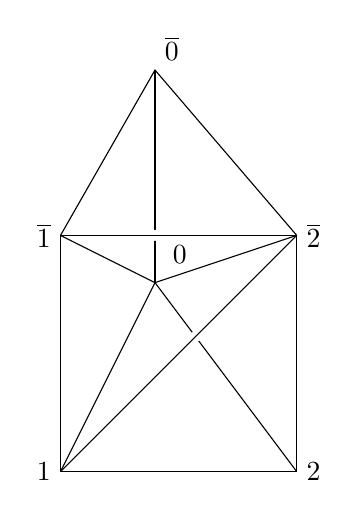
\begin{tikzpicture}[scale=0.6]%, every node/.style={transform shape}]

\draw [name path=f1,opacity=0] (0,0) node[left] {$0$} -- (5,0) -- (5,5) -- (0,5) -- cycle;
\draw (0,5) -- (2,4) -- (0,0);
\draw (0,5) -- (2,8.5) -- (5,5);
\draw [name path=f2,opacity=0] (5,5) -- (0,0);
\draw (2,4) -- (5,5);
\draw [name path=b1] (2,8.5) -- (2,4) ;
\draw [name path=b2] (2,4) -- (5,0);
\path [name intersections = {of=f1 and b1,by=inter1}];
\path [name intersections = {of=f2 and b2,by=inter2}];
\filldraw [white] (inter1) circle (3pt);
\filldraw [white] (inter2) circle (3pt);
\draw (0,0) -- (5,0) -- (5,5) -- (0,5) -- cycle;
\draw (5,5) -- (0,0);

%% From https://tex.stackexchange.com/q/111660/
% \draw [name path=a, opacity=0] (0,0) -- (2,2);% line that will be repeated
% \draw [name path=b] (0,2) -- (2,0);
% \path [name intersections={of=a and b,by=inter}];
% \filldraw [white] (inter) circle (2pt);
% \draw (0,0) -- (2,2);% line repeated
\node[label=50:$0$] at (2,4) {};
\node[left] at (0,0) {$1$};
\node[right] at (5,0) {$2$};

\node[above right] at (2,8.5) {$\overline{0}$};
\node[left] at (0,5) {$\overline{1}$};
\node[right] at (5,5) {$\overline{2}$};
\end{tikzpicture}} 
the $2$-simplices given by three-element subsets of these, the $1$-simplices given by two-element
subsets of these, and six $0$-simplices,
$0, 1, 2, \overline{0},\overline{1}$ and $\overline{2}$. This can visualised as at right.

More generally, given any $n$, we can define a triangulation of the space $I\times \Delta^n$ using an 
analogous recipe: the desired $\Delta$-set has $n+1$ $(n+1)$-simplices labelled by the lists
\begin{align*}
& 0,1,\ldots, n,\overline{n}\\
& 0,1,\ldots,n-1,\overline{n-1},\overline{n}\\
&\vdots\\
& 0,\overline{0},\overline{1},\ldots,\overline{n}\\
\end{align*}
such that the $n+2$ vertices of each simplex are ordered as shown,
and the lower-dimensional simplices are labelled by the lists arising from applying the face 
maps $d_i$ that omit the $i^{th}$ element from the list.


Given a $\Delta$-set $X_\bullet$ we can define a sequence of $R$-modules 
\[
	\cdots \to R^{X_n} \xrightarrow{\delta_n} R^{X_{n+1}} \to \cdots
\]
where for $g\colon X_n\to R$, 
\[
	\delta_n(g) = \sum_{i=0}^n (-1)^ig\circ d_i^{n+1}\colon X_{n+1}\to R
\]

\begin{lemma}
This sequence is a complex, so that $\delta_{n+1}\circ \delta_n = 0$.
\end{lemma}

\begin{proof}
Exercise!
\end{proof}

We denote this complex by $C^\bullet(X_\bullet,R)$, and call it the \emph{simplicial cochain
complex} of the $\Delta$-set $X_\bullet$.

Now notice that given a function $\alpha\colon A\to B$ of sets, there is an $R$-linear map 
$\alpha^*\colon R^B\to R^A$ defined on $(g\colon B\to R)\mapsto (g\circ \alpha\colon A\to R)$. 
And, given another function $\beta\colon B\to C$, we have 
$\alpha^*\circ \beta^* = (\beta\circ \alpha)^*\colon R^C\to R^A$. Thus we have a kind of 
functoriality, but where the source and target get flipped, and the order of composition likewise. 
This is summed up by saying we have a functor $R^{(-)}\colon \Set^{op}\to \Mod_R$, where the 
${}^{op}$ is a reminder that everything gets flipped on applying the functor.

\begin{lemma}
There is a functor $C^\bullet(-,R)\colon \Delta\Set^{op}\to \Cplx_R$.
\end{lemma}

\begin{proof}
One just needs to check that given $f\colon X_\bullet \to Y_\bullet$, we have 
$\delta_nf_n^* = f_{n+1}^*\delta_n$, which is a direct computation.
\end{proof}

As a result, we can define the cohomology modules of a $\Delta$-set.

\begin{definition}
The $n^{th}$ cohomology module $H^n(X_\bullet,R)$ with coefficients in $R$ is the $n^{th}$ cohomology
of the complex $C^\bullet(X_\bullet,R)$, and so is a functor $H^n(-,R)\colon \Delta\Set^{op}\to \Mod_R$.
\end{definition}

Note that since $R^\emptyset = 0$, the trivial module, it is immediate that for an 
$n$-dimensional $\Delta$-set $X_\bullet$ we have $H^k(X_\bullet,R) = 0$ for all $k>n$. 
Infinite-dimensional $\Delta$-sets may or may not have nontrivial cohomology modules in 
infinitely-many dimensions. 

Another immediate corollary of this definition is that a finite $\Delta$-set has finitely-generated
cohomology modules.\marginnote{or more generally, a $\Delta$-set with finitely many simplices in dimension $n$ has $H^n$ finitely-generated}

\begin{rem}
In practice, the only rings $R$ we will consider are $\ZZ$, $\RR$ and $\ZZ/2$.
\end{rem}

\begin{rem}
Given a finite $\Delta$-set, with all of the face maps explicitly described, to calulate
its cohomology modules is purely a calculational effort in combinatorics and linear algebra.
However, the effort required may be significant, so there are tools we shall develop that will
assist. Further, for an $\Delta$-set that is not finite, for instance, being 
infinite-dimensional or having infinitely-many $n$-simplices for a given $n$, we cannot rely 
on simple linear algebra to help us much. This will become important later, when we define
the cohomology modules of a general topological space, without using $\Delta$-sets.
\end{rem}

Given a map of rings $\alpha\colon R\to S$ and a set $A$, recall that there is an $R$-linear map 
$R^A\to S^A$ given by $g\mapsto \alpha\circ g$. This is $R$-linear as we can consider
the $S$-module $S^A$ to be an $R$-module via $\alpha$.
As a result, for a $\Delta$-set $X_\bullet$, we can apply this to the singular cochain complex 
of $X_\bullet$ at each slot.

\begin{lemma}
For a map of rings $\alpha\colon R\to S$ there is a map of complexes 
$C^\bullet(X_\bullet,R)\to C^\bullet(X_\bullet,S)$, and for fixed $X_\bullet$ this is functorial
in $\alpha$.
\end{lemma}

Since a map of complexes gives a map between cohomology modules, we get from $\alpha$ as above
an $R$-linear map $H^n(X_\bullet,R) \to H^n(X_\bullet,S)$, the \emph{change of coefficients} map.

\begin{example}
Consider the inclusion $\ZZ\to\RR$, which gives rise to maps 
$H^n(X_\bullet) \to H^n(X_\bullet,\RR)$. Notice that the domain is an abelian group, and in particular
can contain torsion subgroups, whereas the codomain is a real vector space. The kernel of this
map is precisely the torsion subgroup $H^n(X_\bullet,\ZZ)_\mathrm{tors} < H^n(X_\bullet,\ZZ)$, and the image is a lattice in
$H^n(X_\bullet,\RR)$.
\end{example}

\begin{example}
We have the quotient maps $\ZZ\to \ZZ/p$ for $p$ a prime, and so get maps
$H^n(X_\bullet,\ZZ) \to H^n(X_\bullet,\ZZ/p)$, where the codomain is now a $\mathbb{F}_p$-vector
space. Now this map destroys any torsion coprime to $p$, so can be useful in trying to focus
on specific phenomena relating to a specific prime number.
\end{example}

\begin{rem}
At the dawn of algebraic topology, the focus was largely on objects similar to finite $\Delta$-complexes
and in that case, one could define the dimension of the vector spaces $H^n(X_\bullet,\RR)$, 
called the \emph{Betti numbers} of $X_\bullet$,
and consider the orders of the cyclic subgroups that defined the finite group 
$H^n(X_\bullet,\ZZ)_\mathrm{tors}$ (under the classification of finitely-generated abelian
groups), called the \emph{torsion coefficients}. These were the way mathematicians at the time
unpacked the information that went into the Euler characteristic, but still these numbers 
were not functorial. It took Emmy Noether and others in the 1920s to emphasise that having 
invariants that are themselves algebraic objects was more important than considering just 
their dimensions or other numeric invariants.
\end{rem}

Going\lecturenum{23} back to thinking about functoriality with respect to maps of 
$\Delta$-sets, consider for $x\in X_n$ ($X_\bullet$ a given $\Delta$-set) the map in 
Example~\ref{eg:name_of_simplex}, $\Delta[n] \to X_\bullet$ We can consider the induced map
on complexes near dimension $n$:
\[
	\xymatrix{
	\ar[r] & R^{X_n} \ar[d] \ar[r]^\delta & R^{X_{n+1}} \ar[r] \ar[d] & \\
	\ar[r] & R^{\Delta[n]_n} \ar[r] & R^{\Delta[n]_{n+1}} \ar[r] &
	}
\]
but $R^{\Delta[n]_n} = R^1 = R$ (as a module) and $R^{\Delta[n]_{n+1}} = R^\emptyset=0$, so we
get an $R$-linear map $C^n(X_\bullet,R) = R^{X_{n+1}} \to R$. This map is precisely 
evaluation at $x\in X_n$.
An important case for us is when we have a chosen\marginnote{this 
really is, under the indended geometric interpretation, a point} basepoint $x\in X_0$. Then
we get a map $C^\bullet(X_\bullet,R)=R^{X_0} \to C^\bullet(\Delta[0],R)$, and the codomain
here is a complex of the form $0\to R \to 0\to \cdots$. This map on passing to 
cohomology gives a map $H^0(X_\bullet,R) \to R$ of $R$-modules. Such a map on an $R$-module $M$
is called an \emph{augmentation} of $M$, and $M\to R$ is called an \emph{augmented module}.
The assignment $(X_\bullet) \mapsto (H^0(X_\bullet,R) \to R)$ is functorial for maps of $\Delta$-set
respecting the chosen basepoints, and where augmentations are preserved on the $R$-module side.
The extra geometric structure contained in the choice of basepoint is reflected by the augmentation.

\begin{rem}
While $\Delta$-sets and their cohomology are not at present helping to define or calculate
cohomology of topological spaces, the tools we are developing will come in handy when we get
to that point. So for the present we will continue to focus on $\Delta$-sets and their associated
complexes. 
\end{rem}

What sort of general results help us to calculate cohomology of $\Delta$-sets? Just as for space,
let us consider the simplest method for constructing a new object from old: disjoint union.

Some observations:
\begin{enumerate}
\item For sets $P$ and $Q$ and a ring $R$, there is a natural isomorphism 
$R^{P\sqcup Q} \xrightarrow{\simeq} R^Q \oplus R^Q$ of $R$-modules.

\item From $\Delta$-sets $X_\bullet$ and $Y_\bullet$ we can make a new $\Delta$-set
$X_\bullet\sqcup Y_\bullet$ with set of $n$-simplices $X_n\sqcup Y_n$.

\item From complexes $A_\bullet$ and $B_\bullet$ of $R$-modules, we can make a new complex
$A_\bullet \oplus B_\bullet$, namely
\[
	\cdots \to A_n\oplus B_n \xrightarrow{\delta^A_n\oplus \delta^B_n} A_{n+1}\oplus B_{n+1} \to \cdots
\]
the \emph{direct sum} of $A_\bullet$ and $B_\bullet$.

\item Given a direct sum of complexes $A_\bullet\oplus B_\bullet$, we have an natural isomorphism
$H^n(A_\bullet\oplus B_\bullet) \xrightarrow{\simeq} H^n(A_\bullet)\oplus H^n(B_\bullet)$.
\end{enumerate}

If we put these ingredients together, we get:
\begin{lemma}
There is a natural isomorphism 
\[
	C^\bullet(X_\bullet\sqcup Y_\bullet,R) \xrightarrow{\simeq}
C^\bullet(X_\bullet,R)\oplus C^\bullet(Y_\bullet,R)
\]
of complexes of $R$-modules.
\end{lemma}

\begin{corollary}
There is a natural isomorphism 
\[
H^(X_\bullet\sqcup Y_\bullet,R) \xrightarrow{\simeq} H^n(X_\bullet,R) \oplus H^n(Y_\bullet,R)
\]
of $R$-modules, for $n=0,1,2,\ldots$.
\end{corollary}

Recalling the situation for the fundamental groupoid $\Pi_1$, we had the result that
$\Pi_1(X\sqcup Y) \simeq \Pi_1(X)\sqcup \Pi_1(Y)$. So, in this case we can reduce computations
to $\Delta$-sets that are not disjoint unions of smaller $\Delta$-sets. One thing to notice 
is that the lemma is legitimately stronger than its corollary, since there might be an induced
isomorphism between the cohomology modules while the complexes are not isomorphism.

The next step up from calculating the fundamental groupoid of a disjoint union is to calculate
the fundamental groupoid of a pushout of spaces: $X = U\cup V$ for neighbourhoods $U,V\subset X$.
More precisely there was a way to get information about $\Pi_1(X)$ from $\Pi_1(U)$, $\Pi_1(V)$ 
and $\Pi_1(U\cap V)$. Things are not so simple now, even ignoring the fact we are working 
with $\Delta$-sets. The following two examples should be in some sense motivational for the 
big tool we are about to develop. 

\begin{example}
Consider the combinatorial surface $\partial\Delta[3]$, with vertices $0,1,2,3$, and 
$n$-simplices given by $(n+1)$-element subsets of this.
Define two sub-$\Delta$-sets $U_\bullet$ and $V_\bullet$ as follows:
\begin{enumerate}
\item $U_\bullet$ has the same vertices as $\partial\Delta[3]$ but only two $2$-simplices: 
$\{0,1,2\}$ and $\{0,1,3\}$, and all the $1$-simplices of $\partial \Delta[3]$ \emph{except}
$\{2,3\}$.
\item $V_\bullet$ also has the same vertices as $\partial\Delta[3]$ but now the pair of $2$-simplices
$\{1,2,3\}$ and $\{0,2,3\}$, and all the $1$-simplices \emph{except} $\{0,1\}$.
\end{enumerate}
The\marginnote{defined to have as set of $n$-simplices $U_n\cap V_n\subset X_n$} 
intersection $U_\bullet\cap V_\bullet$ is then $1$-dimensional---that is a directed graph---with 
vertices $\{0,1,2,3\}$ and edges $\{0,2\}$, $\{0,3\}$, $\{1,2\}$ and $\{1,3\}$ (ordered from
lower to higher label).\marginnote{this geometrically realises to a circle} Now, in principle,
we already know, or suspect we know, the cohomology modules of $U_\bullet$, $V_\bullet$ and 
$U_\bullet\cap V_\bullet$ as the first two triangulate $I^2$, and the latter triangulates a 
circle. Then it would be nice if we could calculate the cohomology of $\partial\Delta[3]$ just
from this information.

From the functoriality of $C^\bullet(-,R)$ we get restriction maps, which in each dimension 
look like
\[
	\xymatrix{
		R^{\partial\Delta[3]_n} \ar[r] \ar[d] & R^{U_n} \ar[d]\\
		R^{V_n} \ar[r] & R^{U_n\cap V_n}
	}
\]
and this square commutes. However, we are in a more of a linear, sequency mood, so will turn
this into the sequence
\begin{align*}
	0\to R^{\partial\Delta[3]_n} \to & R^{U_n}\oplus R^{V_n} \to R^{U_n\cap V_n}\to 0\\
	g\mapsto & (g\big|_{U_n},g\big|_{V_n})\\
		& (f,h) \mapsto f\big|_{U_n\cap V_n} - h\big|_{U_n\cap V_n}
\end{align*}
It is a short and simple exercise to check that in fact this sequence is in fact exact. This then
gives a short exact sequence of complexes
\[
0\to C^\bullet(\partial\Delta[3],R) \to C^\bullet(U_\bullet,R) \oplus C^\bullet(V_\bullet,R) \to C^\bullet(U_\bullet\cap V_\bullet,R) \to 0
\]
We want to know the cohomology of the leftmost non-zero complex, but we (in principle) have
only calculated the cohomology of the other two complexes.
\end{example}

The above argument works perfectly well for an arbitrary $\Delta$-set $X_\bullet$ and 
sub-$\Delta$-sets $U_\bullet$ and $V_\bullet$ such that $X_n = U_n \cup V_n$, to give a short
exact sequence of complexes of $R$-modules
\[
0\to C^\bullet(X_\bullet,R) \to C^\bullet(U_\bullet,R) \oplus C^\bullet(V_\bullet,R) \to C^\bullet(U_\bullet\cap V_\bullet,R) \to 0
\]

For the second example, we want to consider how we might calculate the cohomology of a quotient
from the cohomology of the original $\Delta$-set and that of the sub-$\Delta$-set that gets squashed.

\begin{example}

Consider now a $\Delta$-set $X_\bullet$ together with a sub-$\Delta$-set $A_\bullet 
\subset X_\bullet$.\marginnote{that is, a \emph{pair} $(X_\bullet,A_\bullet)$} Morally 
speaking, we might have $X_\bullet$ triangulating some space, and $A_\bullet$ 
triangulating a subspace. We can form the quotient space $|X_\bullet|/|A_\bullet|$, but 
it is not immediately clear that we can form a sensible $\Delta$-set 
$X_\bullet/A_\bullet$ that is a quotient of $X_\bullet$ so that this triangulates the 
topological quotient. Assume for now that there \emph{is} a $\Delta$-set 
$X_\bullet/Y_\bullet$ with set of $n$-simplices $X_n/Y_n$, and a quotient map 
$X_\bullet\to X_\bullet/Y_\bullet$ of $\Delta$-sets. Can we calculate 
$H^n(X_\bullet/Y_\bullet,R)$ from $H^n(X_\bullet,R)$ and $H^n(Y_\bullet,R)$?

Notice that given a set $X$ and a subset $i\colon Y\hookrightarrow X$, we get a set $X/Y := X/(y_1\sim y_2)$ for all $y_i\in Y$,
and there is a function $q\colon X\to X/Y$. The set $X/Y$ has a canonical basepoint $\pt = [y]\in X/Y$ for any $y\in Y$.
We get $R$-linear maps given by precomposition:
\[
	R^{X/Y} \xrightarrow{q^*} R^X \xrightarrow{i^*} R^Y 
\]
where the left map is injective, and the right map is surjective. However, this is not even a complex,
as the image of $q^*$ is not contained in the kernel of $i^*$!

Examining the situation, we see that the image of $q^*$ consists of those functions $X\to R$
that are constant on $Y$, whereas the kernel of $i^*$ consists of those functions that are
$0$ on $Y$. Moreover, recalling that $X/Y$ has a canonical basepoint, the module $R^{X/Y}$ 
has an augmentation, namely evaluation on that basepoint: $\ev_\pt\colon R^{X/Y}\to R$. The 
kernel of this map includes into $R^X$ as precisely those functions that are in the kernel
of $i^*$! This example may not be telling us something deep, other than to get a complex that
plays well with quotient we may need to play around with the kernel a bit: in one sense the 
`correct' module of functions on $X/A$ is really $\ker i^*$, so as to get an exact sequence
\[
	0\to \ker i^* \to R^X \to R^A\to 0
\] 
Phrased this way, we don't even need to consider the quotient set $X/A$ in order to get a module
from it. And this also helps with the issue above, in that it's not clear to what extent 
$X_\bullet/Y_\bullet$ is a good construction. 

Hence,\lecturenum{24} given a pair $(X_\bullet,A_\bullet)$, with inclusion function $i\colon A_\bullet \hookrightarrow X_\bullet$, we can consider the 
(surjective) restriction map
\[
	C^\bullet(X_\bullet,R) \xrightarrow{i^*} C^\bullet(A_\bullet,R) \to 0
\]
and its kernel $\ker(i^*)$ acts like virtual functions on $X_\bullet/A_\bullet$, without 
having to define this $\Delta$-set. Moreover, we then have a short exact sequence of 
complexes of $R$-modules, analogously to the previous example.
\end{example}

Before continuing, it is worth noting that in fact the last construction does make sense

\begin{lemma}
Given a map of complexes $\varphi\colon A_\bullet \to B_\bullet$, the degreewise kernels
$\ker(\varphi_n) \subseteq A_n$ assemble into a complex $\ker(\varphi)$, using the restriction
of $A_n \to A_{n+1}$ to $\ker(\varphi_n)$.
\end{lemma}

Using this lemma, we can define a complex associated to the pair $(X_\bullet,A_\bullet)$.

\begin{definition}
Given a pair $(X_\bullet,A_\bullet)$ denote by $C^\bullet(X_\bullet,A_\bullet;R)$ the 
complex $\ker(i^*)$ as above, the simplicial relative cochain complex of the pair.
\end{definition}

Both of these examples are special cases of a general principle: given a short exact sequence 
of complexes
\[
	0\to A_\bullet \to B_\bullet \to C_\bullet \to 0
\]
(of $R$-modules, say) then we might wish to calculate $H^n(A_\bullet)$, but only know 
$H^n(B_\bullet)$ and $H^n(C_\bullet)$. Or we might know $H^n(A_\bullet)$ and 
$H^n(C_\bullet)$, and want to calculate $H^n(B_\bullet)$. In the finite setting, this 
might be merely an issue of computational efficiency, but in general we need to deal 
with infinitely-generated $R$-modules, where simple linear algebra techniques start to 
break down. So we will prove a general result using \emph{homological 
algebra}\marginnote{Homological algebra is the area of algebra that deals with the 
interaction of sequences, maps of sequences, commutative diagrams of algebraic objects 
with certain `exactness' properties, and how one can calculate various objects including 
(co)homology groups} that relates all these cohomology groups.

\begin{rem}
If you get anything out of this section of the course, the following result is probably 
it, because you can apply it to your own setting to get a long exact sequence. Or it 
might be the case there is a standard long exact sequence\marginnote{or, in the case of 
$K$-theory, a long exact sequence that folds back on itself} in your area, and it 
probably arose from this theorem, so it's a good idea to understand how the abstract 
proof goes. Together with the long exact sequence of homotopy groups associated to a 
fibre bundle, this is one of the major computational tools until you get to spectral 
sequences, which are super powerful, but also much less intuitive.
\end{rem}

\begin{theorem}\label{thm:alg_Mayer-Vietoris}
Given a short exact sequence 
\[
        0\to A_\bullet \xrightarrow{i} B_\bullet \xrightarrow{\pi} C_\bullet \to 0
\]
of $R$-modules, there is a long exact sequence
\[
\cdots \xrightarrow{\delta^{k-1}} H^k(A_\bullet) \xrightarrow{H^k(i)} H^k(B_\bullet) \xrightarrow{H^k(\pi)} H^k(C_\bullet)
\xrightarrow{\delta^k} H^{k+1}(A_\bullet) \xrightarrow{H^{k+1}(i)} (B_\bullet) \to \cdots
\]
of $R$-modules.
\end{theorem}

The proof of this theorem we will give uses a famous lemma in homological algebra, the \emph{Snake 
Lemma}.\marginnote{there is a small zoo of lemmas named after animals, other examples 
being the Salamander Lemma and the Snail Lemma}

\begin{lemma}[Snake Lemma]
\label{snakeLemma}
Given a commutative diagram 
\[
	\xymatrix{
	& A \ar[r]^i \ar[d]^\alpha & B \ar[r]^\pi \ar[d]^\beta & C \ar[r] \ar[d]^\gamma & 0 \\
	0\ar[r] & A' \ar[r]_{i'} & B' \ar[r]_{\pi'} & C
	}
\]
of $R$-modules where the rows are exact, there is an exact sequence
\[
	\ker\alpha \to \ker\beta \to \ker\gamma \xrightarrow{\delta} \coker\alpha 
	\to \coker\beta \to \coker\gamma
\]
of $R$-modules (see Figure~\ref{fig:snake_lemma}).
\end{lemma}

This is a major tool, so the full proof is rather lengthy with lots of details, but at each stage there is generally
only one or two things to try.

\begin{figure}
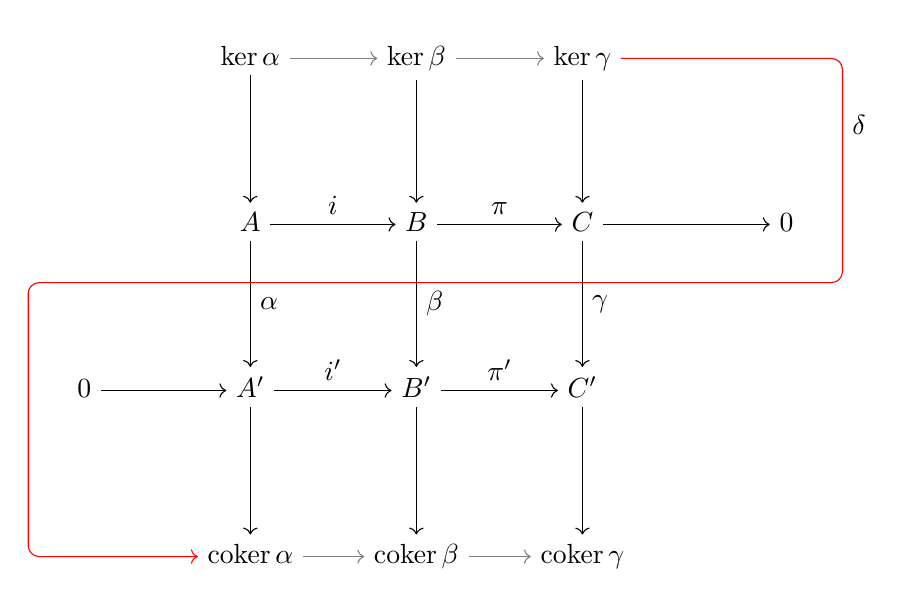
\begin{tikzpicture}%[>=triangle 60]
\matrix[matrix of math nodes,column sep={60pt,between origins},row
sep={60pt,between origins},nodes={asymmetrical rectangle}] (s)
{
&|[name=ka]| \ker \alpha &|[name=kb]| \ker \beta &|[name=kc]| \ker \gamma \\
%
&|[name=A]| A &|[name=B]| B &|[name=C]| C &|[name=01]| 0 \\
%
|[name=02]| 0 &|[name=A']| A' &|[name=B']| B' &|[name=C']| C' \\
%
&|[name=ca]| \coker \alpha &|[name=cb]| \coker \beta &|[name=cc]| \coker \gamma \\
};
\draw[->] (ka) edge (A)
          (kb) edge (B)
          (kc) edge (C)
          (A) edge node[auto] {\(i\)} (B)
          (B) edge node[auto] {\(\pi\)} (C)
          (C) edge (01)
          (A) edge node[auto] {\(\alpha\)} (A')
          (B) edge node[auto] {\(\beta\)} (B')
          (C) edge node[auto] {\(\gamma\)} (C')
          (02) edge (A')
          (A') edge node[auto] {\(i'\)} (B')
          (B') edge node[auto] {\(\pi'\)} (C')
          (A') edge (ca)
          (B') edge (cb)
          (C') edge (cc)
;
\draw[->,gray] (ka) edge (kb)
               (kb) edge (kc)
               (ca) edge (cb)
               (cb) edge (cc)
;
\draw[->,red,rounded corners] (kc) -| node[auto,text=black,pos=.7]
{\(\delta\)} ($(01.east)+(.5,0)$) |- ($(B)!.35!(B')$) -|
($(02.west)+(-.5,0)$) |- (ca);
\end{tikzpicture}
\caption{The classic Snake Lemma diagram}
  \label{fig:snake_lemma}
  %\zsavepos{pos:textfig}
  \setfloatalignment{c}
\end{figure}


\begin{proof}
We need to do a number of things:
\begin{enumerate}
\item Construct the function $\delta \colon \ker\gamma \to \coker\alpha$
\item Prove this is an $R$-module homomorphism
\item Show $\im(\ker\alpha \to \ker\beta) = \ker(\ker\beta \to \ker\gamma)$
\item Show $\im(\ker\beta \to \ker\gamma) = \ker(\delta)$
\item Show $\im(\delta) = \ker(\coker\alpha \to \coker\beta)$
\item Show $\im(\coker\alpha \to \coker\beta) = \ker(\coker\beta \to \coker\gamma)$
\end{enumerate}

For the present, I will do 1., 4.\ and 5. Items 3.\ and 6.\ are a bit more 
straightforward, as they don't involve $\delta$. And, given the techniques here, item 
2.\ should be a not-too-challenging exercise. The main technique here is called `diagram 
chasing', as it involves starting with an element in one module, and applying 
homomorphisms or exactness properties to cook up elements of other nearby modules, and 
repeat, chasing the new elements until we find one in a module we are interested in. 

Since we want a function $\delta\colon \ker\gamma \to \coker\alpha$, we will start with 
a given element $c\in \ker\gamma \subseteq C$ and aim to end up with an element in 
$\coker\alpha$ Since we know $\pi$ is surjective, there is a $b\in B$ such that $\pi(b) 
= c$. Then consider $\beta(b) \in B'$: applying $\pi'$ we get $\pi'(\beta(b)) = 
\gamma(\pi(b)) = \gamma(c)=0$, so that $\beta(b) = i'(a'_b)$ for a unique $a'_b \in A'$. 
Then we have $[a'_b] \in \coker\alpha$. But is it unique? I hear you ask. Well, what 
choices did we make along the way? Only the fact that there is not a unique $b$ such 
that $\pi(b)=c$. So consider another $\tilde b \in B$ such that $\pi(\tilde b) = c$. We 
get $\beta(\tilde b)$, as before, and there is a unique $a'_{\tilde b} \in A'$ such that 
$i'(a'_{\tilde b}) = \beta(\tilde b)$. So we get another element $[a'_{\tilde b}]\in 
\coker\alpha$. But, $\pi(b - \tilde b)= \pi(b) - \pi(\tilde b) = c -c = 0$, and 
$\ker\pi=\im i$, so there is some $\underline{a}\in A$ such that $i(\underline{a}) = b - 
\tilde b$, or rather, $b = \tilde b + i(\underline{a})$. So now apply $\beta$ to get 
$i'(a_b) = \beta(b) = \beta(\tilde b + i(\underline{a})) = \beta(\tilde b) + 
\beta(i(\underline{a})) = i'(a'_{\tilde b}) + i'(\alpha(\underline{a})) = i'(a'_{\tilde b} 
+ \alpha(\underline{a}))$. But $i'$ is injective, so that $a_b = a'_{\tilde b} + 
\alpha(\underline{a})$. But this means that $[a'_b] = [a'_{\tilde b}]$, and so from $c\in 
\ker\gamma$ we have found a unique element of $\coker\alpha$. Thus we have a function
$\delta\colon \ker\gamma \to \coker\alpha$, as required.



One needs to then check this is an $R$-module homomorphism, by comparing 
$\delta(c_1+c_2)$ and $\delta(c_1) + \delta(c_2)$ etc, using exactness in various ways as in 
the previous paragraph. This is an exercise for the keen reader.

We can now check the exactness of the sequence. Assume $c\in \ker \gamma$ such that 
$\delta(c)=0$, that is, $[a'_b] = 0 \in \coker\alpha$ for some $b\in B$ such that 
$\pi(b)=c$. But this means $a'_b = \alpha(\underline{a})$. But since $\beta(b) = 
i'(a'_b) = i'(\alpha(\underline{a})) = \beta(i(\underline{a}))$, we get $b - 
i(\underline{a}) \in \ker\beta$. And $\pi(b - i(\underline{a})) = \pi(b) - 
\pi(i(\underline{a})) = c$. Thus $c\in \im(\ker \beta \to \ker \gamma)$ and $\ker\delta 
\subseteq \im(\ker \beta \to \ker \gamma)$

Conversely, assume that $c = \pi(b)$ where $b\in \ker\beta$. Then $\delta(c) = [a'_b]$ 
for $i'(a'_b) = \beta(b)$, but as $i'$ is injective, $a'_b = 0$, hence $\delta(c)=0$. 
Thus $\im(\ker \beta \to \ker \gamma)\subseteq \ker\delta$, and so $\im(\ker \beta \to 
\ker \gamma)= \ker\delta$.

Now consider an arbitrary $c\in \ker\gamma$, and the image of $\delta(c)$ in 
$\coker\beta$. This is precisely $[i'(a'_b)] = [\beta(b)] = 0$, so that $\im\delta 
\subseteq \ker(\coker\alpha \to \coker\beta)$. Now consider a $[a']\in \coker\alpha$ 
such that $[i'(a')]=0 \in \coker\beta$. But then this means that $i'(a') = \beta(b)$ for 
some $b\in B$. If we take $c:= \pi(b)$, then $\delta(c) = [a']$, so that $\im\delta
=\ker(\coker\alpha \to \coker\beta)$.

The proof that we have exactness in the other positions is left for the keen reader.
\end{proof}

To apply the Snake Lemma to the proof of Theorem~\ref{thm:alg_Mayer-Vietoris}, we need 
to cook up a diagram with the appropriate properties. Despite the temptation to apply 
the Snake Lemma to (two rows of) the short exact sequence of complexes, this is not the 
correct thing to do, since then the kernels and cokernels are not the cohomology groups 
in the Theorem.

\begin{lemma}\label{lemma:setup_for_algMV}
The commutative diagram
\[
	\xymatrix{
	&A_k/\delta_{k-1}^A(A_{k-1}) \ar[r] \ar[d]^{\delta_k^A} & B_k/\delta_{k-1}(B_{k-1}) 
	\ar[r] \ar[d]^{\delta_k^B} & C_k/\delta_{k-1}^C(C_{k-1}) \ar[r] \ar[d]^{\delta_k^C} & 0\\
	0\ar[r] & \ker(\delta_{k+1}^A) \ar[r]& \ker(\delta_{k+1}^B) \ar[r] & \ker(\delta_{k+1}^C)	
	}
\]
satisfies the hypotheses of the Snake Lemma, that is, the rows are exact.
\end{lemma}

\begin{proof}
Exercise, for now.
\end{proof}

\begin{proof}{(of Theorem~\ref{thm:alg_Mayer-Vietoris})}

First notice that $\ker(A_k/\delta_{k-1}^A(A_{k-1}) \to \ker\delta_{k+1}^A) = 
\ker(A_k/\delta_{k-1}^A(A_{k-1}) \to A_{k+1})$. But this is isomorphic to $\ker(A_k\to 
A_{k+1})/\delta_{k-1}^A(A_{k-1}) = H^k(A_\bullet)$.\marginnote{exercise!}
Similarly, we have $\im(A_k/\delta_{k-1}^A(A_{k-1}) \to \ker\delta_{k+1}^A) = \im(A_k \to \ker\delta_{k+1}^A$ and hence the cokernel is $H^{k+1}(A_\bullet)$.

Using Lemma~\ref{lemma:setup_for_algMV}, we get an exact sequence
\[
	H^k(A_\bullet) \to H^k(B_\bullet) \to H^k(C_\bullet) \xrightarrow{\delta^k}
	H^{k+1}(A_\bullet) \to H^{k+1}(B_\bullet) \to H^{k+1}(C_\bullet)
\]
for each $k$. We\marginnote{For a collection of exact sequences $L_{k-1} \to M_{k-1} \to 
N_{k-1} \to L_k \to M_k \to N_k$, $k\in \ZZ$ (where the maps are re-used) 
 there is a long exact sequence 
$\cdots \to N_{k-2} \to L_{k-1} \to M_{k-1} \to
N_{k-1} \to L_k \to M_k \to N_k \to L_{k+1} \to \cdots$ (Exercise)}
can put these together as $k$ varies to get one long exact sequence as in 
the statement of the theorem.
\end{proof}

One nice result is that given two diagrams of the sort that go into the Snake Lemma, and 
maps between each of the corresponding modules making all the possible cubes commute, 
there are maps between the kernels and cokernels that appear in the exact sequence, 
giving a map between the complexes.\marginnote{the Snake Lemma is thus `natural'} This 
means that given two short exact sequences of complexes, and maps between \emph{them}, 
there is a map between the long exact sequences. This might happen, for instance, if one 
is changing the coefficient ring in the cohomology of $\Delta$-sets, and one is in the 
situation of one of the two motivational examples. Or, one might have a map of pairs 
$(X_\bullet,A_\bullet) \to (Y_\bullet,B_\bullet)$ of $\Delta$-sets, so that each of them 
gives rise to a short exact sequence of complexes, and the map between the pairs induces a 
map between the short exact sequences.


The\lecturenum{25} cohomology of the complex of relative simplicial cochains turns out to
be quite important, and also gives more flexibility in the definition of cohomology of a $\Delta$-set.
We recover the complex $C^\bullet(X_\bullet,R)$ by taking $A_\bullet=\emptyset$, hence
the complex $C^\bullet(X_\bullet,\emptyset;R)$.

\begin{definition}
Given a pair $(X_\bullet,A_\bullet)$ of $\Delta$-sets, its \emph{relative cohomology} is
$H^k(X_\bullet,A_\bullet;R) := H^k(C^\bullet(X_\bullet,A_\bullet;R))$.
\end{definition}

\begin{example}\label{eg:dim_minus_one_skeleton_rel_cochains}
Given $X_\bullet$ a finite-dimensional $\Delta$-set of dimension $n$, then 
$(X_\bullet,\sk_{n-1}X_\bullet)$ is a pair, and so we get the relative cochain complex
\[
	0\to C^1(X_\bullet,\sk_{n-1}X_\bullet;R) \to \cdots \to C^{n-1}(X_\bullet,\sk_{n-1}X_\bullet;R) \to C^n(X_\bullet,\sk_{n-1}X_\bullet;R) \to 0
\]
but for $k < n$, $\sk_{n-1}X_k = X_k$, so that $C^k(X_\bullet,\sk_{n-1}X_\bullet) = \ker(\id_{R^{X_k}}) = 0$
Moreover, $\sk_{n-1}X_n = \emptyset$, so that $C^n(X_\bullet,\sk_{n-1}X_\bullet;R) = \ker(R^{X_n} \to R^\emptyset=0) = R^{X_n}$. Hence the complex $C^\bullet(X_\bullet,\sk_{n-1}X_\bullet;R)$ 
consists entirely of copies of the zero $R$-module, except at position $n$,\marginnote{This is often denoted $R^{X_n}[n]$ in homological algebra} where it is the module of 
$R$-valued functions on $X_n$. Thus 
\[
	H^k(X_\bullet,\sk_{n-1}X_\bullet;R) = \begin{cases}
						0 & k\neq n\\
						R^{X_n} & k=n
						\end{cases}
\]
\end{example}

The proof of the following lemma follows immediately from the definitions.

\begin{lemma}
For $k < n$, $H^k(\sk_nX_\bullet,R) \simeq H^k(X_\bullet,R)$.
\end{lemma}

As a result, every cohomology module of a given $\Delta$-set can be calculated as a cohomology 
module of a finite-dimensional $\Delta$-set, albeit the dimension of the $\Delta$ grows with the 
dimension the cohomology module sits in.\marginnote{A more sophisticated result shows the cohomology modules can be approximated, in a precise way, by cohomology modules of \emph{finite} $\Delta$-sets. This will take us too far afield to cover now.}

\begin{prop}
Given a pair $(X_\bullet,A_\bullet)$ of $\Delta$-sets, there is a long exact sequence of $R$-modules
\[
\xymatrix{%adapted from https://tex.stackexchange.com/a/16516/141
    0 \ar[r] & H^0(X_\bullet,A_\bullet;R) \ar[r] & H^0(X_\bullet,R) \ar[r] & H^0(A_\bullet,R) \ar@{->} `r/8pt[d] `/10pt[l] `^dl[ll] `^r/1pt[dll] [dll] \\
             & H^1(X_\bullet,A_\bullet;R) \ar[r] & H^1(X_\bullet,R)\ar[r] &\cdots \\
                &&\cdots \ar[r] & H^{k-1}(A_\bullet,R)
                \ar@{->} `r/8pt[d] `/10pt[l] `^dl[ll] `^r/1pt[dll] [dll] \\
             & H^k(X_\bullet,A_\bullet;R) \ar[r] & H^k(X_\bullet,R) \ar[r] & \cdots 
}
\]
\end{prop}


\begin{example}
Consider for instance the pair $(\Delta[n],\partial\Delta[n])$\marginnote{A special case of 
Example~\ref{eg:dim_minus_one_skeleton_rel_cochains}, as $\partial\Delta[n] = 
\sk_{n-1}\Delta[n]$} We have $H^k(\Delta[n],\partial\Delta[n];R) = 0$ for $k\neq n$, and since 
$\Delta[n]$ has a single $n$-simplex, $H^n(\Delta[n],\partial\Delta[n];R)=R$. The long exact 
sequence breaks up into small pieces, namely
\[
	0\to H^k(\Delta[n],R) \xrightarrow{\simeq} H^k(\partial\Delta[n],R) \to 0
\]
for $k<n-1$, which we already knew on general grounds from the above example, and
\[
0\to H^{n-1}(\Delta[n],R) \to H^{n-1}(\partial\Delta[n],R) \to R \to 
H^n(\Delta[n],R) \to 0
\]
From this we can see that the cohomology module $H^n(\Delta[n],R)$ is a quotient of the rank-one module $R$, so it is not so big.\marginnote{in fact it is trivial, but we haven't proved that yet!}
\end{example}

If we think of relative cohomology as a kind of cohomology of a `virtual quotient' by a sub-$\Delta$-set,
then if take the pair to be $(X_\bullet,\{x\})$, where $x\in X_0$, then we really can take the quotient squashing $\{x\}$ to a point: it changes nothing!
But the relative cohomology really is different from the ordinary cohomology, so the naive idea that it
looks like a kind of quotient really needs a bit more subtle interpretation.

\begin{example}
Consider a really simple $\Delta$-set, namely $\partial\Delta[1]$, which has two $0$-simplices, and
nothing else. Call these $x_0$ and $x_1$, and look at the relative cochain complex. The only non-zero
module is
\[
C^0(\partial\Delta[1],\{x_0\};R) = \ker(R^{\{x_0,x_1\}} = R^2\xrightarrow{\pr_2} R^{\{x_0\}} = R) = R
\]
and so $H^0(\partial\Delta[1],\{x_0\};R) = R$ (and all other $H^k$ are $0$). Compare this to 
$H^0(\partial\Delta[1],R) = R^2$.
\end{example}

More generally, given a $0$-dimensional $\Delta$-set with $n+1$ $0$-simplices and a chosen 
basepoint, the relative cohomology will be a rank $n$ free $R$-module. So this counts the number 
of points \emph{apart from the specified basepoint}. 

This case comes up often enough that it warrants a special name. We call a $\Delta$-set with a specified
$0$-simplex a \emph{pointed $\Delta$-set}.

\begin{definition}
Given a pointed $\Delta$-set $(X_\bullet,x)$, the \emph{reduced cohomology} is the 
relative cohomology $H^k(X_\bullet,x;R)$.
\end{definition}

\begin{example}
Define the $\Delta$-set $Pt_\bullet$ to be $Pt_n = \ast$\marginnote{this is infinite-dimensional, with one $n$-simplex for every $n\in \NN$} 
for all $n\geq 0$, with all face maps the identity function. Thus $C^n(Pt_\bullet,R) = R$ for all $n$.
We need to calculate the maps $\delta_n \colon R\to R$ that appear in the complex. Firstly, we think
of the elements of $R$ as given by functions $\ast \to R$ (of sets), so precomposition with $d_i=\id_\ast$ becomes the identity function on $R$. Thus
\[
g \stackrel{\delta_n}{\mapsto} \sum_{i=0}^{n+1} (-1)^i g = \begin{cases}
0 & n\text{ even}\\
g & n\text{ odd}
\end{cases}
\]
Thus the complex is
\[
	0\to R \xrightarrow{0} R \xrightarrow{\id}R \xrightarrow{0} R \xrightarrow{\id}R \to \cdots
\]
and so $H^0(Pt_\bullet,R) = R$, but $H^k(Pt_\bullet,R) = 0$ for all $k>0$. But $Pt_\bullet$ has a canonical basepoint, and $H^k(Pt_\bullet,\ast;R) = 0$ for all $k$.
\end{example}

You can think of $Pt_\bullet$ in the last example as a kind of infinite-dimensional fat point, or perhaps
a kind of contractible `space', even though we haven't got a notion of continuous deformation of
$\Delta$-sets. This is more of a combinatorial analogue, or, better, and algebraic one, since $\Delta$-sets
are really just a way to construct examples of complexes, which are our simpler, algebraic,  versions of spaces.
We can define an analogue of a map of complexes being weak homotopy equivalence as follows.

\begin{definition}
A map of complexes $f\colon A_\bullet\to B_\bullet$ is called a \emph{quasi-isomorphism} if
$H^k(f)\colon H^k(A_\bullet) \to H^k(B_\bullet)$ is an isomorphism for all $k$.
\end{definition}

\begin{example}
The map $C^\bullet(Pt_\bullet,R)\to C^\bullet(\sk_0Pt_\bullet,R)$ induced by the inclusion is a quasi-isomorphism, despite the domain being nontrivial in all non-negative positions, and the latter
being concentrated in a single position.
\end{example}

We will need just one more homological algebra lemma\marginnote{not named after an animal this time!} that
is very useful in practice.

\begin{lemma}[5 Lemma]
Given a diagram of $R$-modules
\[
	\xymatrix{
	A\ar[r]^f \ar[d]^\alpha & B \ar[r]^g \ar[d]^\beta & C \ar[r]^h \ar[d]^\gamma & D \ar[r]^k \ar[d]^\delta & R \ar[d]^\varepsilon \\
	A' \ar[r]_{f'} & B' \ar[r]_{g'} & C' \ar[r]_{h'} & D' \ar[r]_{k'} & E'
	}
\]
where the rows are exact, then if $\alpha$ is surjective, $\beta$ and $\delta$ are isomorphisms, and $\varepsilon$ is injective, then $\gamma$ is an isomorphism.
\end{lemma}

\begin{proof}
The proof is, as usual, a diagram chase. We split the proof into two steps, each of which only uses half
of the assumptions:
\begin{enumerate}

\item If $\varepsilon$ is injective, and $\beta$ and $\delta$ are surjective, then $\gamma$ is 
surjective. Consider $c' \in C'$, and choose some $d\in D$ such that $\delta(d) = h'(c')$. 
Consider $\varepsilon(k(d)) = k'(\delta(d)) = k'(h'(c')) = 0$. Since $\varepsilon$ is injective, 
this means $k(d)=0$, and since the top row is exact, this means that $d\in \ker(k) = \im(h)$, so 
that there exists $c\in C$ such that $d=h(c)$. It's not immediately true that $\gamma(c) = c'$, 
so let us compare them: $h'(c'-\gamma(c)) = h'(c') - h'(\gamma(c)) = \delta(d) - \delta(h(c)) = 
0$. By exactness of the bottom row, this means that $c' - \gamma(c) = g'(b')$ for some $b'\in 
B$. But as $\beta$ is surjective, $b' = \beta(b)$ for some $b\in B$. That is, $c' - \gamma(c) = 
g'(\beta(b)) = \gamma(g(b))$. We can rearrange this so that $c' = \gamma(c) + \gamma(g(b)) = \gamma(c+g(b))$, and hence $\gamma$ is surjective.

\item If $\alpha$ is surjective, and $\beta$ and $\delta$ are injective, then $\gamma$ is injective. This is an exercise in dualising the above steps.\qedhere
\end{enumerate}
\end{proof}

Now to revisit the idea of Euler characteristic of a finite $\Delta$-set, which is, recall, the
sum\marginnote{the sum terminates, as $|X_d| = 0$ for all large enough $d$}
\[
	\chi(X_\bullet) = \sum_{d=0}^\infty (-1)^d |X_d|
\]
A key idea introduced at the beginning of this section was that we wanted to replace numerical invariants,
such as cardinality of finite sets by vector spaces, or more generally modules, so that dimension replaced
cardinality. We now have a different way to construct a numerical invariant from a $\Delta$-set, namely
using the dimensions of the cohomology modules, in the case when we take $R = \RR$, say.\marginnote{any characteristic zero field would do}
Thus we can define the \emph{cohomological Euler characteristic} to be
\[
	\chi^{coh}(X_\bullet) := \sum_{d=0}^\infty (-1)^d \dim H^d(X_\bullet,\RR)
\]
as long as this sum exists. While now this implies that $H^d(X_\bullet,\RR)=0$ for all large enough $d$,
we certainly don't need to have $X_\bullet$ finite, or even finite-dimensional, as the example of $Pt_\bullet$ shows. In that case, $\chi^{coh}(X_\bullet) = 1$.
We can also consider finite-dimensional but infinite $\Delta$-sets, for instance a triangulation of $\RR$ by $1$-simplices.

\begin{example}
Let $L_\bullet$ be the directed graph with $L_0 = \ZZ$ and $L_1 = \ZZ$, where $d_0(n) = n+1$ and $d_1(n) = n$.
This has an edge from $n$ to $n+1$ for each $n$. Given $g\in \RR^{L_0} = \RR^\ZZ$, 
$\delta_0(g)(n) = g(n+1) - g(n)$. So $\delta(g) = 0$ precisely if $g$ is constant, hence $\ker(\delta_0) = H^0(L_\bullet,\RR) = \RR$.

And, given $h\in \RR^{L_1} = \RR^\ZZ$, define $g(0) = 0$, and then use $g(n+1) = h(n) + g(n)$ to
define $g\colon \ZZ\to \RR$ for all nonzero $n\in\ZZ$, so that $\delta_0(g) = h$. Thus $\coker(\delta_0) = H^1(L_\bullet,\RR) = 0$. All other real-coefficient cohomology vector spaces are trivial,
so that $\chi^{coh}(L_\bullet) = 1$.
\end{example}

However, now we have two numerical invariants of a finite $\Delta$-set, namely $\chi$ and $\chi^{coh}$,
and it is not immediately obvious how they relate. Thankfully, they coincide, and so we can just call
this the Euler characteristic

\begin{prop}
For a finite $\Delta$-set $X_\bullet$, we have $\chi(X_\bullet) = \chi^{coh}(X_\bullet)$
\end{prop}

\begin{proof}
First, $|X_d| = \dim \RR^{X_d}$, and consider the part of the complex near there:
\[
	\RR^{X_{d-1}} \xrightarrow{\delta_{d-1}} \RR^{X_d} \xrightarrow{\delta_d} \RR^{X_{d+1}}
\] 
We can, using the standard inner product,  break $\RR^{X_d}$ into a direct sum:
\begin{align*}
\RR^{X_d}& = \ker\delta_d\oplus \im \delta_d\\
	 & = \begin{cases}
		H^d(X_\bullet,\RR) \oplus \im\delta_{d-1} \oplus \im\delta_d & d > 0\\
		H^0(X_\bullet,\RR) \oplus \im \delta_0 & d=0
	    \end{cases}
\end{align*}
We can unify these two cases if we agree that $H^{-1}(X_\bullet,\RR) = 0$. Then we have
\[
	\dim \RR^{X_d} = \dim H^d(X_\bullet,\RR) + \dim \im\delta_{d-1} + \dim\delta_d
\]
and so
\begin{align*}
\chi(X_\bullet) & = \sum_{d=0}^\infty (-1)^d |X_\bullet|\\
		& = \sum_{d=0}^\infty (-1)^d \dim \RR^{X_d}\\
		& = \sum_{d=0}^\infty (-1)^d \dim H^d(X_\bullet,\RR) + 
			\sum_{d=0}^\infty (-1)^d\left(\dim\im\delta_{d-1} + \dim\im\delta_d \right)\\
		& = \sum_{d=0}^\infty (-1)^d \dim H^d(X_\bullet,\RR) \\
		& = \chi^{coh}(X_\bullet)
\end{align*}
\end{proof}

We thus can drop the superscript on $\chi^{coh}$ and just talk about \textbf{the} Euler characteristic
of a $\Delta$-set.

\begin{rem}
This proof can be adapted pretty much verbatim to show that for a complex $V_\bullet$ of finite-dimensional 
vector spaces of finite length, say
\[
	0 \to V_m \to V_{m+1} \to \cdots \to V_{m+N} \to 0
\]
then
\[
	\sum_{d=m}^{m+N} (-1) \dim V_d = \sum_{d=m}^{m+N} (-1)^d H^d(V_\bullet).
\]
\end{rem}

Recall\lecturenum{26} the geometric realisation of a $\Delta$-set $X_\bullet$:
\[
	|X_\bullet| = \left(\bigsqcup_{n=0}^\infty \disc(X_n) \times \Delta^n\right)_{\big/\sim}
\]
This space has a set of distinguished maps $\Delta^n \to |X_\bullet|$, namely for a given $x\in X_n$, 
we have the composite
\[
	\Delta^n \to \disc(X_n) \times \Delta^n \into \bigsqcup_{n=0}^\infty \disc(X_n) \times \Delta^n \to |X_\bullet|
\]
Note also that precomposing this map with $\partial_i\colon \Delta^{n-1} \into \Delta^n$ gives another
map in the distinguised class, corresponding to $d_i(x) \in X_{n-1}$.

Note also that if we have a smooth manifold $M$ (for instance an open set of $\RR^n$) and $\omega$ is
a differential $k$-form on $M$, then this determines a function\marginnote{by a smooth function on $\Delta^k$
here it is enough to assume it is smooth on the interior and extends continuously to the boundary}
\begin{align*}
C^\infty(\Delta^k,M) &\to \RR\\
(f\colon \Delta^k\to M) & \mapsto \int_{\Delta^k} f^*\omega
\end{align*}
Thus this gives a function from $k$-forms on $M$ to the vector space $\RR^{C^\infty(\Delta^k,M)}$. 
This function also interacts well with the exterior derivative and, by Stokes' theorem, the restriction
of the primitive of an exact form to the boundary.

For a general topological space $X$, we are somewhere in the neighbourhood of these two ideas: since we do 
not have distinguished maps $\Delta^n \to X$, we should consider \emph{all} maps and then functions on
the set of these.

\begin{definition}
Let $X$ be a topological space. The \emph{singular cochain complex} of $X$ with coefficients in the 
ring $R$, denoted $C^\bullet(X,R)$  is given by
\[
	0 \to R^{\Top(\Delta^0,X)} \xrightarrow{\delta} R^{\Top(\Delta^1,X)} \xrightarrow{\delta} R^{\Top(\Delta^2,X)}\to \cdots
\]
where $\delta(g) = \sum_{i=0}^n (-1)^i g\circ \partial_i$. The defines a functor $\Top^{op} \to \Cplx_R$.
Given a map $f\colon X\to Y$, where the induced map $R^{\Top(\Delta^k,Y)} \to R^{\Top(\Delta^k,X)}$ is given by precomposing with the induced $\Top(\Delta^k,X) \to \Top(\Delta^kY)$.

The \emph{singular cohomology} of $X$ with coefficients in $R$ is the cohomology of this complex:
\[
	H^n(X,R) := H^n(C^\bullet(X,R))
\]
and hence gives functors $H^n(-,R) \colon \Top^{op} \to \Mod_R$.
\end{definition}

These modules are \emph{huge} (in general). For example, take $X=I$ and $R=\ZZ/2$, and then 
$|C^1(I,\ZZ/2)| = 2^{|\Top(\Delta^1,I)|} = 2^{|\RR|}$, but, as we shall see in a moment, $H^1(I,\ZZ/2)=0$. 
Hence we \emph{must} rely on theorems to calculate the singular cohomology, unlike the much easier case
of cohomology of $\Delta$-sets.

However, here is the (more of less) only example we can calculate from the definition
\begin{example}
Let $X=\pt$. Then $\Top(\Delta^k,\pt) = \ast$, so that the singular cochain complex 
is\marginnote{we've seen this before!}
\[
0 \to R \xrightarrow{0} R \xrightarrow{\id} R \xrightarrow{0} R\xrightarrow{\id} \cdots
\]
which has cohomology $H^0(\pt,R) = R$ and $H^k(\pt,R) = 0$ for $k>0$.
\end{example}

Just as for $\Delta$-sets, we have relative cohomology, which is useful for the additional flexibility
it affords.

\begin{definition}
For $(X,A)$ a pair of spaces, the \emph{relative singular cochain complex} $C^\bullet(X,A;R)$ is the kernel of $i^*\colon C^\bullet(X,R) \to C^\bullet(A,R)$
where $i\colon A\into X$ is the inclusion. This gives a functor $\Top^{(2),op}\to \Cplx_R$. We then define the \emph{relative singular cohomology}
$H^k(X,A;R) = H^k(C^\bullet(X,A;R))$, which is functorial for maps of pairs of spaces.
\end{definition}

Note that we recover ordinary singular cohomology of $X$ as the relative cohomology of the pair 
$(X,\emptyset)$. Using the same argument as for relative cohomology of $\Delta$-sets, we get

\begin{prop}
Given a pair $(X,A)$ of spaces, there is a long exact sequence
\[
0\to H^0(X,A;R) \to H^0(X,R) \to H^0(A,R) \to H^1(X,A;R) \to H^1(X,R) \to \cdots
\]
of $R$-modules.
\end{prop}

\begin{proof}
There is a short exact sequence of complexes
\[
	0\to C^\bullet(X,A;R) \to C^\bullet(X,R)\to C^\bullet(A,R) \to 0
\]
and then apply Theorem~\ref{thm:alg_Mayer-Vietoris}.
\end{proof}

Let $(X,x)$ be a pointed space, and consider the long exact sequence of the relative cohomology of
 the pair $(X,\pt) = (X,\{x\})$. Since $H^k(\pt,R) = 0$ for positive $k$, the long exact sequence breaks up into
\[
0\to H^0(X,\pt;R) \to H^0(X,R) \to H^0(\pt,R) = R \to H^1(X,\pt;R) \to H^1(X,R) \to 0
\]
and $0\to H^k(X,\pt;R) \xrightarrow{\simeq} H^k(X,R) \to 0$ for $k>1$. From the fragment at the 
start of the exact sequence, we see that $H^0(X,\pt;R) \to H^0(X,R)$ is injective, and this is the 
inclusion of the kernel of the map $H^0(X,R) \to R$. Thus $H^0(X,\{x\};R) = \ker(H^0(X,R) \to R)$.
For simplicity, we denote $H^k(X,\{x\};R)$ by $H^k(X,x;R)$, and call it the \emph{reduced cohomology}
of the pointed space $(X,x)$.


\begin{rem}
We also have the result that $H^1(X,R)$ is the quotient of $H^1(X,x;R)$ by the image of 
$R\to H^1(X,x;R)$, but to say definitively what this is we would need to study the construction
of this map. 
\end{rem}

\begin{example}
For a discrete space $S$ with chosen basepoint $p\in S$, then $H^0(S,p;R) \simeq R^{S\setminus\{p\}}$.
In particular, $H^0(\pt,\pt;R) = R^\emptyset = 0$. 
\end{example}

Since maps of pairs $(X,x) \to (Y,y)$ are just pointed maps, we have that reduced cohomology is a 
functor $H^k(-;R)\colon\Top_*^{op} \to \Mod_R$.\marginnote{Exercise!} Note particularly that 
we only have functoriality for pointed maps.


Here's a first result that would help calculate (relative) cohomology

\begin{prop}
Given pairs of spaces $(X,A)$ and $(Y,B)$, there is a canonical isomorphism
\[
	H^k(X\sqcup Y,A\sqcup B;R) \xrightarrow{\simeq} H^k(X,A:R)\oplus H^k(Y,B;R)
\]
for all $k$. Even better: there is a canonical isomorphism of complexes
\[
	C^\bullet(X\sqcup Y,A\sqcup B;R) \xrightarrow{\simeq} C^\bullet(X,A:R)\oplus C^\bullet(Y,B;R)
\]
that, on passing to cohomology, give the previous isomorphisms.
\end{prop}

\begin{proof}
This is because $\Top(\Delta^k,X\sqcup Y) = \Top(\Delta^k,X)\sqcup \Top(\Delta^k,Y)$, and the 
earlier observation that $R^{P\sqcup Q} \simeq R^P\oplus R^Q$ for any sets $P$ and $Q$.
\end{proof}

Of course, we get the analogous result for plain cohomology by looking at pairs $(X,\emptyset)$ and 
$(Y,\emptyset)$.

Here is a much more powerful and difficult result. Recall that we write $f^*$ generically for $H^k(f)$.

\begin{theorem}\label{thm:homotopy_invariance_cohom}
If the maps $f,g\colon X\to Y$ are homotopic, then 
\[
	f^* = g^*\colon H^k(Y,R) \to H^k(X,R)
\]
for all $k$.
\end{theorem}

I will give a few corollaries of this before discussing what goes into the proof, and how we get the 
above theorem from a stronger statement about complexes. The proofs of the following are applications
of functoriality and the above theorem.

\begin{corollary}
If $X$ and $Y$ are homotopy equivalent, via $f\colon X\leftrightarrows Y:g$, say, then 
$f^* = (g^*)^{-1}$ and $H^k(X,R)$ and $H^k(Y,R)$ are isomorphic for all $k$.
\end{corollary}

\begin{corollary}
If a space $X$ is contractible, then $H^k(X,R) = 0$ for $k>0$ and $H^k(X,R) \simeq R$. More precisely,
if $X$ is contractible to $x\in X$, then $H^k(X,R) \to H^k(\{x\},R)$ is an isomorphism for all $k$,
and hence $H^k(X,x;R) = 0$ for all $k$.
\end{corollary}

\begin{corollary}
Given a pointed space $X$ with a path $\gamma\colon x\rightsquigarrow x'$, the two induced maps 
$H^0(X,R) \to H^0(\pt,R) = R$ given by the inclusion of $x$ and $x'$ are equal, so that 
$H^0(X,x;R) = H^0(X,x';R)$. Thus reduced cohomology only depends on the path component of the basepoint,
not the basepoint specifically.
\end{corollary}

We saw earlier the concept of quasi-isomorphism, which is an analogue for complexes of weak homotopy
equivalence. But for spaces we have the stronger notion of homotopy of maps, and this should be reflected
by some construction for complexes.

\begin{definition}
Let $f,g\colon A_\bullet \to B_\bullet$ be maps of complexes. A \emph{cochain homotopy} from $f$ 
to $g$ is a collection of functions $\{h_n\colon A_n \to B_{n-1}\}$ satisfying the identities
\[
	\delta^B_{n-1}h_n + h_{n+1}\delta^A_n = f_n - g_n
\]
\end{definition}

\begin{lemma}
If there is a cochain homotopy from $f$ to $g$, both maps $A_\bullet\to B_\bullet$, then $H^k(f) = H^k(g)$.
\end{lemma}

\begin{proof}
An element in $H^k(A_\bullet)$ is the equivalence class of some $c\in A_k$ such that $\delta^A_k(c) = 0$
so
\begin{align*}
H^k(f)([c]) & = [f_k(c)]\\
	& = [g_k(c) + \delta^B_{k-1}(h_k(c)) + h_{k+1}(\delta^A_k(x))]\\
	& = [g_k(c)] + [\delta^B_{k-1}(h_k(c))] \\
	& = [g_k(c)]\\
	& = H^k(g)([c])
\end{align*}
\end{proof}

Here is a stronger version of Theorem~\ref{thm:homotopy_invariance_cohom}:

\begin{theorem}
If the maps $f,g\colon X\to Y$ are homotopic, then there is a cochain homotopy between the two induced maps
$C^\bullet(Y,R) \to C^\bullet(X,R)$.
\end{theorem}

The proof is reasonably detailed, but constructs an actual such cochain homotopy. Matters are 
simplified somewhat because one can immediately reduce to the case $Y = I\times X$ and the two 
functions being the inclusions $X\simeq \{i\}\times X \to I\times X$ for $i=0,1$. This is 
because of functoriality and the given homotopy $H\colon I\times X \to Y$. Further, one can reduce 
a lot of the work to the case $X=\Delta^k$, and an explicit triangulation of $I\times \Delta^k$, so
that the inclusion maps $\Delta^k \to I\times \Delta^k$ come from maps of $\Delta$-sets. Then it is messy
combinatorics to make sure the required identity holds.


Let\lecturenum{27} us consider for a short time again the reduced cohomology, which as noted above is functorial for
pointed maps. For an arbitrary space $X$, there is of course a canonical map $X\xrightarrow{!_X} \pt$, which induces a map in cohomology $R=H^0(\pt,R) \to H^0(X,R)$. Moreover, since for any map $f\colon X\to Y$ we have $!_Y \circ f = !_X$, the induced map in cohomology $H^0(Y,R) \to H^0(X,R)$ commutes with these maps from $R$. This is somewhat reminiscent of the situation with reduced cohomology, except now we have a map \emph{from} $R$, not \emph{to} $R$. But what is this map?

\begin{ex}
Given a space $X$, $H^0(X,R) \simeq R^{[\pt,X]}$, that is, functions that are constant on path-components. Moreover, given $f\colon X\to Y$, the induced map $H^0(Y,R) \to H^0(X,R)$ is given by precomposition with $[\pt,X]\to [\pt,Y]$.
\end{ex}

Thus $R = H^0(\pt,R) \to H^0(X,R)$ sends $r\in R$ to the constant function on $X$ with value $r$---assuming $X$ is not empty---so we shall denote it by $\mathrm{const}$. Further, given $x\in X$, the map $!$ is a retraction to $x\colon \pt \to X$, so that $!_X \circ x=\id_X$. Thus we have $R \xrightarrow{\mathrm{const}} H^0(X,R) \xrightarrow{\ev_x} R$ is the identity map on $R$, and so $\mathrm{const}$ is injective.

\begin{definition}
A \emph{left splitting} of a short exact sequence $0\to A \xrightarrow{i} B \xrightarrow{\pi} C \to 0$ of $R$-modules is a map $r\colon B\to A$ such that $r\circ i = \id_A$.
\end{definition}

Thus we have a short exact sequence $0 \to R\to H^0(X,R) \to \coker(\mathrm{const}) \to 0$, and $\ev_x$ is a left splitting.

\begin{lemma}
Given a left splitting $r$ of a short exact sequence $0\to A \xrightarrow{i} B \xrightarrow{\pi} C \to 0$, the map $(r,\pi)\colon B\to A\oplus C$ is an isomorphism, and $C \simeq \coker(r)$.
\end{lemma}
 
As a result, from a choice $x\in X$ we get an isomorphism $\coker(\mathrm{const})\simeq H^0(X,x;R)$. Since the map $\mathrm{const}$ is canonical, and doesn't depend on the choice of $x$, it turns out that reduced cohomology is essentially independent of the choice of basepoint.\marginnote{the submodule $H^0(X,x;R)\subseteq H^0(X,R)$ can be different for different choices of $x\in X$, though} Thus we can redefine reduced cohomology to be $\widetilde{H}^k(X,R) := \coker(H^k(\pt,R) \to H^k(X,R))$; for $k>0$, $\widetilde{H}^k(X,R)\simeq H^k(X,R)$, but otherwise $H^0(X,R) \simeq \widetilde{H}^0(X,R) \oplus R$. Further, this is functorial for all maps of spaces, not pointed maps.

\begin{example}
Given any path-connected space $X$ we get $\widetilde{H}^0(X,R) = 0$ for all $k$. In particular, if $X$ is contractible, then $\widetilde{H}^k(X,R) = 0$ for all $k$.
\end{example}

\begin{example}\label{eg:reduced_cohom_S0}
For the $0$-sphere $S^0$, we have $\widetilde{H}^0(S^0,R) = R$ and $\widetilde{H}^k(S^0,R) = 0$ for $k > 0$.
\end{example}

Since we are in the realm of looking at long exact sequences, let us consider the topological space version of Mayer--Vietoris for a union of two subspaces. Take $\mathcal{U} = \{U,V\}$ an open cover of the space $X$. There is a pushout diagram
\[
	\xymatrix{
	U\cap V \ar[r]^{i_V} \ar[d]_{i_U} & V \ar[d]^{j_V} \\
	U \ar[r]_{j_U} & X
	}
\]
We can define a map
\begin{align}\label{eq:restr_to_intersection}
C^\bullet(U,R) \oplus C^\bullet(V,R) & \to C^\bullet(U\cap V,R)\\
(f,g) & \mapsto i^*_U f - i^*_Vg
\end{align}
which turns out to be onto: given $\widetilde{f}\colon \Top(\Delta^n,U\cap V) \to R$, we can define a function
$f\colon \Top(\Delta^n,U) \to R$ by extension by zero, as $\Top(\Delta^n,U\cap V)$ is naturally a subset of $\Top(\Delta^n,U)$. Then $(f,0) \mapsto \widetilde{f}$. So if we define $C^\bullet_\mathcal{U}(X,R)$ as the kernel of (\ref{eq:restr_to_intersection}), we get a short exact sequence of complexes
\[
0 \to C^\bullet_\mathcal{U}(X,R) \to C^\bullet(U,R) \oplus C^\bullet(V,R) \to C^\bullet(U\cap V,R) \to 0
\]
We can identify this kernel as something concrete, namely 
\[
	C^k_\mathcal{U}(X,R) := \{f\colon \Top(\Delta^k,X) \to R\mid f(\sigma)=0\text{ if $\sigma\colon \Delta^k\to X$ doesn't factor through $U$ or $V$}\}
\]
The following result is key, but also has a very long and complicated proof
\begin{prop}
The inclusion $C^\bullet_\mathcal{U}(X,R) \to C^\bullet(X,R)$ is a quasi-isomorphism, so that
\[
	H^k(C^\bullet_\mathcal{U}(X,R)) \xrightarrow{\simeq} H^k(X,R).
\]
\end{prop}

\begin{proof}
This follows from reasoning similar to Hatcher's Proposition~2.21, albeit using cohomology, not homology.
\end{proof}

The idea of the proof is that given $\Delta^k \to X$, one can interatively retriangulate $\Delta^k$ by more and smaller simplices so that eventually you can break up $\Delta^k$ into a collection of functions on small simplices, each of which lands (by an application of the Lebesgue covering lemma) inside one of the open subsets $U$ or $V$. This is formally similar to how one can integrate over a simplex in a manifold by covering a manifold by charts, by breaking the simplex up into parts each of which land inside a chart, and then integrate each bit and add them up.

\begin{theorem}{(Mayer--Vietoris)}\label{thm:mayer-vietoris}
Given an open cover $\{U,V\}$ of the space $X$, there is a long exact sequence
\[
0\to H^0(X,R) \to H^0(U,R)\oplus H^0(V,R) \to H^0(U\cap V,R) \to H^1(X,R) \to H^1(U,R)\oplus H^1(V,R) \to \cdots
\]
of $R$-modules, and similarly with reduced cohomology, starting
\[
0\to \widetilde{H}^0(X,R) \to \widetilde{H}^0(U,R)\oplus \widetilde{H}^0(V,R) \to \widetilde{H}^0(U\cap V,R) \to H^1(X,R) \to \cdots
\]
\end{theorem}

Here is a key example.

\begin{example}
Cover the sphere $S^n$ ($n\geq 1$) by two open sets $D^n_+$ and $D^n_-$, both homeomorphic to discs (hence contractible). Their intersection is homeomorphic to $S^{n-1}\times J$, for $J$ a small open interval, hence homotopic to $S^{n-1}$. We thus get by the Mayer--Vietoris theorem a long exact sequence
\[
\hspace{-1.5cm}0\to \widetilde{H}^0(S^n,R) \to \widetilde{H}^0(D^n_+,R)\oplus \widetilde{H}^0(D^n_-,R) \to \widetilde{H}^0(S^{n-1}\times J,R) \to H^1(S^n,R) \to H^1(D^n_+,R)\oplus H^1(D^n_-,R) \to H^1(S^{n-1}\times J,R) \to \cdots
\]
but since $D^n_\pm$ are contractible, this breaks up into pieces. Firstly, $0\to \widetilde{H}^0(S^n,R) \to 0$, hence $\widetilde{H}^0(S^n,R) =0$, which we knew already, as $S^n$ is path connected. Then for $k>0$ we have
\[
0\to \widetilde{H}^0(S^{n-1},R) \to H^1(S^n,R) \to 0
\]
and 
\[
0\to H^{k-1}(S^{n-1},R) \to H^k(S^n,R) \to 0
\]
for all $k > 1$. Hence we can attack this problem by induction as (combining the two cases) $\widetilde{H}^{k-1}(S^{n-1},R) \simeq \widetilde{H}^k(S^n,R)$. If we take $k=n$, then this gives
\[
\widetilde{H}^{n-1}(S^{n-1},R) \simeq \widetilde{H}^n(S^n,R)
\]

By Example~\ref{eg:reduced_cohom_S0} we know the reduced cohomology of $S^0$, namely $\widetilde{H}^0(S^0,R) = R$, so that $\widetilde{H}^n(S^n,R) = H^n(S^n,R) = R$ for all $n \geq 1$.
\end{example}






\end{document}
